%%%%%%%%%%%%%%%%%%%%%%%%%%%%%%%%%%%%%%%%%
% Masters/Doctoral Thesis 
% LaTeX Template
% Version 1.43 (17/5/14)
%
% This template has been downloaded from:
% http://www.LaTeXTemplates.com
%
% Original authors:
% Steven Gunn 
% http://users.ecs.soton.ac.uk/srg/softwaretools/document/templates/
% and
% Sunil Patel
% http://www.sunilpatel.co.uk/thesis-template/
%
% License:
% CC BY-NC-SA 3.0 (http://creativecommons.org/licenses/by-nc-sa/3.0/)
%
% Note:
% Make sure to edit document variables in the Thesis.cls file
%
%%%%%%%%%%%%%%%%%%%%%%%%%%%%%%%%%%%%%%%%%

%----------------------------------------------------------------------------------------
%	PACKAGES AND OTHER DOCUMENT CONFIGURATIONS
%----------------------------------------------------------------------------------------

\documentclass[11pt, oneside]{Thesis} % The default font size and one-sided printing (no margin offsets)

\graphicspath{{Pictures/}} % Specifies the directory where pictures are stored

\usepackage[spanish]{babel}
\usepackage[dvipsnames, table]{xcolor}
\definecolor{mygray}{gray}{0.9}
\usepackage{minted}
\usemintedstyle{friendly}
\usepackage{breakurl}
\usepackage{tabularx}
\usepackage{array, graphicx}
\usepackage{booktabs}
\usepackage{pifont}
\usepackage{changepage}
\usepackage{tabu}
\usepackage{bmpsize}
\usepackage{booktabs}% http://ctan.org/pkg/booktabs
\newcommand{\tabitem}{~~\llap{\textbullet}~~}
\usepackage{float}
\usepackage{url}
\usepackage[square, numbers, comma, sort&compress]{natbib} % Use the natbib reference package - read up on this to edit the reference style; if you want text (e.g. Smith et al., 2012) for the in-text references (instead of numbers), remove 'numbers' 
\hypersetup{urlcolor=blue, colorlinks=true} % Colors hyperlinks in blue - change to black if annoying
\title{\ttitle} % Defines the thesis title - don't touch this

\begin{document}

\frontmatter % Use roman page numbering style (i, ii, iii, iv...) for the pre-content pages

\setstretch{1.0} % Line spacing of 1.3
%\renewcommand{\baselinestretch}{1.0}
%\linespread{1.0}

% Define the page headers using the FancyHdr package and set up for one-sided printing
\fancyhead{} % Clears all page headers and footers
\rhead{\thepage} % Sets the right side header to show the page number
\lhead{} % Clears the left side page header

\pagestyle{fancy} % Finally, use the "fancy" page style to implement the FancyHdr headers

\newcommand{\HRule}{\rule{\linewidth}{0.5mm}} % New command to make the lines in the title page

% PDF meta-data
\hypersetup{pdftitle={\ttitle}}
\hypersetup{pdfsubject=\subjectname}
\hypersetup{pdfauthor=\authornames}
\hypersetup{pdfkeywords=\keywordnames}

%----------------------------------------------------------------------------------------
%	TITLE PAGE
%----------------------------------------------------------------------------------------

\begin{titlepage}
\begin{center}
\textsc{\LARGE \univname}\\[1.5cm] % University name


\begin{figure}[htbp]
	\centering
		
\includegraphics[width=0.5\textwidth]{Figures/logo.png}
		\rule{35em}{0.5pt}
\end{figure}


\textsc{\Large Proyecto Integrador}\\[0.5cm] % Thesis type
\textsc{\Large Ingeniería en Computación}\\[0.5cm] % Thesis type

\HRule \\[0.4cm] % Horizontal line
{\huge \bfseries \ttitle}\\[0.4cm] % Thesis title
\HRule \\[1cm] % Horizontal line
 
\begin{minipage}[t]{0.4\textwidth}
\begin{flushleft} \large
\emph{Autores:}{ Gianfranco \textsc{Barbiani}}\\ % Author name - remove the \href bracket to remove the link
\emph{Matrícula: }{36372639}
\\{ Loreley Nahir \textsc{Bustamante}}\\ % Author name - remove the \href bracket to remove the link
\emph{Matrícula: }{32298299}
\end{flushleft}
\end{minipage}
\begin{minipage}[t]{0.4\textwidth}
\begin{flushright} \large
\emph{Director:}\\{Mgt. Ing. Miguel \textsc{Solinas}} \\
 % Supervisor name - remove the \href bracket to remove the link  
\emph{Codirector:}\\{\supname}
\\~\\~\\ % Supervisor name - remove the \href bracket to remove the link  
\end{flushright}
\end{minipage}

\facname\\~\\ % Research group name and department name
 
{\large \today}\\ % Date
%\includegraphics{Logo} % University/department logo - uncomment to place it
\vfill
\end{center}
\end{titlepage}

\clearpage % Start a new page

\pagebreak

% \vspace*{\fill}
% \begingroup
% \begin{center}
% \textit{Para Juan, el amor de mi vida.} 
% \end{center}
% \endgroup
% \vspace*{\fill}
% \pagebreak

%----------------------------------------------------------------------------------------
%	ABSTRACT PAGE
%----------------------------------------------------------------------------------------
\newpage
\vspace*{\fill}
\begin{center}
\section*{Resumen}
\end{center}
Los avances tecnológicos y la reducción en los costos han hecho proliferar la industria aeroespacial, incluyendo la disponibilidad de imágenes satelitales. La lista de proveedores de éstas es extensa e incluye no solo al sector público, cuyas imágenes están disponibles para todos los ciudadanos, sino también, más recientemente, al privado, donde se destacan por ejemplo los sitios Satellogic y Kagel.
Las imágenes satelitales poseen una serie de particularidades con respecto a otro tipo de imágenes. Las primeras son matrices de varios millones de píxeles, con una basta variedad de resoluciones de terreno, dependiendo del proveedor y de la banda espectral en la que fue obtenida. La resolución de terreno determina el tamaño de los objetos que pueden detectarse en el. Esas imagenes son multiespectrales y existe un arreglo de pixeles por cada banda espectral utilizada. Estos suelen incluir los usuales colores Rojo, Verde y Azul (RGB), pero también Infrarrojos de onda cercana, Infrarrojos de onda corta, Termal o las bandas Pancromáticas por nombrar algunas. El análisis combinado de estas bandas habilita la construcción y estudio de índices, tales como vegetación, agua, suelo o índices termales, que luego facilitan posibles soluciones alrededor de, por ejemplo, el uso del suelo y la detección de suelo cubierto. Por esto y muchas otras cosas, las imágenes satelitales se están convirtiendo en una increíble fuente de información contextual para muchas industrias y vale la pena invertir en ellas.

Afortunadamente, los avances tecnológicos con los que vivimos en este mundo nos permiten proveer soluciones innovadoras, una de estas tecnologías  en los últimos años ha cobrado particular relevancia: la Inteligencia Artificial (AI en sus siglas en inglés). A grandes rasgos una AI es un agente flexible que percibe su entorno y lleva a cabo acciones que maximicen sus posibilidades de éxito en algún objetivo o tarea. Dentro de lo que la AI se destaca la popularidad del uso de Computer Vision  o Visión por computadoras, como uno de los campos de investigación más populares en este momento y se encuentra en la intersección de muchas materias académicas tales como Ciencias de la Computación (Gráficos, Algoritmos, Teoría, Sistemas, Arquitectura), Matemáticas (Recuperación de Información, Aprendizaje Automático), Ingeniería (Robótica, Procesamiento de Imágenes), Física (Óptica ), Biología (neurociencia) y psicología (ciencia cognitiva). 

Las tareas de reconocimiento visual como la clasificación, localización y detección de imágenes son componentes clave de la visión por computadora. Y es aquí donde el presente proyecto cobra vida: Como punto de partida, se dispone de un set de imágenes satelitales de público acceso que describen diferentes áreas del territorio argentino. Con ellas se plantea, entonces, hacer uso de la Ciencia de Datos, en análisis estadístico, y machine learning para implementar una Inteligencia Artificial que permita analizar el contenido de una imagen satelital y devuelva los resultados basados ​​en el contenido mejor coincidente.
\vspace*{\fill}

\newpage
% \vspace*{\fill}

% \begin{center}
% \section*{Agradecimientos}
% \end{center}

% Especialmente le agradezco a Juan, mi compañero de vida, que hizo lo imposible para ayudarme a afrontar mi vida en Argentina, mi carrera y este trabajo final.

% Agradezco a mi familia por su apoyo y comprensión al tener una hija que estudió una carrera en otro continente.

% Agradezco a los amigos y compañeros con los que estudié, preparé trabajos y viví años inolvidables. Especialmente me gustaría mencionar a Cecilia, con la que formamos un equipo soñado y aprendimos muchísimo juntas.

% Agradezco a mis directores, Matias Cuenca del Rey y Gustavo Wolfmann ya que sin su supervisión, confianza y paciencia este proyecto no hubiera sido posible.

% Finalmente, me gustaría agradecer a todos los docentes de la Facultad de Ciencias Exactas Físicas y Naturales por su compromiso con la enseñanza y por darnos todos los días lo mejor de ellos.

% \vspace*{\fill}
% \newpage

%----------------------------------------------------------------------------------------
%	LIST OF CONTENTS/FIGURES/TABLES PAGES
%----------------------------------------------------------------------------------------

\pagestyle{fancy} % The page style headers have been "empty" all this time, now use the "fancy" headers as defined before to bring them back

\lhead{\emph{Índice General}} % Set the left side page header to "Contents"
\tableofcontents % Write out the Table of Contents

\lhead{\emph{Índice de ilustraciones}} % Set the left side page header to "List of Figures"
\listoffigures % Write out the List of Figures

\lhead{\emph{Lista de Tablas}} % Set the left side page header to "List of Tables"
\listoftables % Write out the List of Tables

%----------------------------------------------------------------------------------------
%	ABBREVIATIONS
%----------------------------------------------------------------------------------------

\clearpage % Start a new page

%\setstretch{1.5} % Set the line spacing to 1.5, this makes the following tables easier to read

%\lhead{\emph{Siglas y Acrónimos}} % Set the left side page header to "Abbreviations"
%\listofsymbols{ll} % Include a list of Abbreviations (a table of two columns)
%{
%\textbf{ledger} & se refiere al conjunto de información almacenado en un Blockchain\\
%\textbf{cluster}\\
%\textbf{script}\\

%\textbf{Acronym} & \textbf{W}hat (it) \textbf{S}tands \textbf{F}or \\
%}


%----------------------------------------------------------------------------------------
%	THESIS CONTENT - CHAPTERS
%----------------------------------------------------------------------------------------

\mainmatter % Begin numeric (1,2,3...) page numbering

\pagestyle{fancy} % Return the page headers back to the "fancy" style

% Include the chapters of the thesis as separate files from the Chapters folder
% Uncomment the lines as you write the chapters

% % Chapter Template

\chapter{Introducción} % Main chapter title

\label{Chapter1} % Change X to a consecutive number; for referencing this chapter elsewhere, use \ref{ChapterX}

\lhead{Capítulo 1. \emph{Introducción}} % Change X to a consecutive number; this is for the header on each page - perhaps a shortened title

\setstretch{1.1} % Line spacing of 1.1
\section{Introducción}

En la Universidad Nacional de Córdoba se generan las llamadas actas de exámenes para dejar constancia de los resultados de las evaluaciones en los turnos de examen. Un acta consta de un encabezado con información sobre la materia a la cual corresponde, la fecha y otros datos necesarios y luego renglones con información sobre los alumnos inscritos junto con la nota correspondiente de cada alumno.
Luego de que se completó y controló el acta, es cerrado y archivado. Además de quedar asentados en papel, las notas también son ingresadas al sistema Guaraní, un sistema de gestión de alumnos utilizado por la UNC.

Como el sistema Guaraní almacena la información ingresada en una base de datos, cualquier persona con los accesos y permisos suficientes puede ser, por ejemplo, un administrador de bases de datos, tiene la posibilidad de modificar la información almacenada. En la actualidad, la integridad de la información en el sistema Guaraní no puede ser garantizada, por lo cual certificados de historias académicas tienen que ser validadas contra las actas en papel. El proceso de validación suele llevar 10 días hábiles.

Una posible forma de automatizar el proceso podría implementarse mediante archivos en formatos legibles para computadoras, como por ejemplo JSON, en conjunto con una firma digital, para garantizar la integridad. Dicha solución, sin embargo, presenta dos problemas: en un ataque contra la disponibilidad de los datos, un administrador podría eliminar una parte de la información sin que esto sea detectado. Eso es especialmente un problema en el caso de actas rectificadas ya que no es posible modificar un acta cerrada, así las actas rectificadas digitales mantienen una firma válida y pueden volver a ser consideradas válidas en el caso de desaparición de su acta rectificativa.

Un Blockchain es una base de datos distribuida de solo escritura que hace uso de mecanismos criptográficos para que la información almacenada sea inmutable y segura. La distribución se logra a través de una red \textit{peer to peer}, a la cual se pueden unir tantos nodos como se desea. Los datos son ordenados de forma cronológica y la automatización se vuelve posible al usar \textit{smart contracts}, programas que son accionados por eventos y pueden provocar cambios en el estado de los datos. De este modo, los problemas de integridad y disponibilidad podrían resolverse.

En respuesta a los problemas mencionados, la presente propuesta de proyecto integrador consiste en el desarrollo de un sistema de validación de información académica en Blockchain como prueba de concepto.

\section{Motivación}

Las motivaciones de llevar a cabo el trabajo integrador presente fueron las siguientes:
\begin{itemize}
    \item La posibilidad de estudiar a una tecnología nueva.
    \item La oportunidad de participar en un proyecto de investigación y potencialmente realizar publicaciones científicas sobre lo estudiado.
    \item  Si bien la tecnología Blockchain se conoce en el ambiente de las criptomonedas, su uso en otros ambientes no está establecido, por lo cual el desarrollo de un prototipo para un ambiente académico resulta de especial interés.
    
\end{itemize}

\section{Marco institucional}

El presente proyecto integrador forma parte del proyecto de investigación de “Tecnologías Blockchain” que cuenta con la participación de la Universidad Nacional de Córdoba y el Laboratorio de Redes y Computadoras. El equipo multidisciplinario de trabajo está compuesto por el Ing. José Daniel Britos, la Ing. Dra. Laura Cecilia Diaz Dávila y varios estudiantes de Ingeniería en Computación. 

El objetivo general del proyecto de investigación es el de explorar la tecnología disruptiva “Blockchain” y sus posibles implementaciones más allá de su implementación original: “las criptomonedas” que dieron origen al concepto de cadena de bloques.

El rol del presente proyecto integrador, dentro del proyecto de investigación, es el de analizar, estudiar y emplear la tecnología Blockchain en un sistema de validación de información académica. Actualmente existe un proyecto semejante de validación de certificados con Blockchain en la Prosecretaría Informática de la UNC.\cite{paper_montes}

\section{Objetivos}

El objetivo principal del presente trabajo es adquirir conocimientos sobre Blockchain y aplicar dichos conocimientos al desarrollar un prototipo para la validación de actas académicas y evaluar ventajas y desventajas de este caso.

\subsection{Objetivos particulares}
\begin{itemize}
    \item Investigar la tecnología Blockchain, su funcionamiento y sus casos de uso a fondo.
    \item Investigar y estudiar diferentes implementaciones y plataformas existentes.
    \item Evaluar en base a los requerimientos, cuál es la implementación o plataforma más adecuada para realizar un prototipo.
    \item Configurar un Blockchain localmente en un ambiente de desarrollo e implementar \textit{smart contracts} que permiten validar actas académicas.
    \item Complementar al Blockchain con una API y una interfaz gráfica para mejorar su usabilidad.
\end{itemize}

\section{Estructura del texto}

A continuación se describe el contenido de cada uno de los capítulos: 
\begin{itemize}
    \item \textbf{Capítulo 1 - Introducción: }El presente capítulo describe el trabajo en palabras generales, junto con motivaciones y objetivos del mismo.
    \item \textbf{Capítulo 2 - Marco Teórico: }El capítulo consta de tres partes: En primer lugar, se explica el funcionamiento y las características únicas de la tecnología Blockchain tomando la criptomoneda Bitcoin como ejemplo, seguido por una primera discusión sobre posibles requerimientos del prototipo. En segundo lugar, se analizan implementaciones alternativas detallando diferencias y similitudes con Bitcoin. Por último, se llega a una conclusión sobre qué plataforma resulta ser la más adecuada para la implementación de un prototipo.
    \item \textbf{Capítulo 3 - Hyperledger Fabric: }El capítulo describe con mayor detalle los componentes importantes y el funcionamiento de la plataforma que se eligió en el capítulo anterior.
    \item \textbf{Capítulo 4 - Análisis y Diseño: }Luego del resumen de una entrevista con el director de Prosecretaría de Informática de la UNC sobre el presente proyecto, se procede a describir las herramientas más importantes a utilizar y a definir los requerimientos del trabajo con mayor detalle.
    \item \textbf{Capítulo 5 - Implementación: }En primer lugar, se describen los pasos de configuración del Blockchain con Hyperledger Fabric junto con el desarrollo de los \textit{smart contracts}. Además, se describe la implementación de la API como también la implementación de la interfaz gráfica de usuario, junto con primeras pruebas del sistema en un ambiente local.
    %Por último, se describen los pasos necesarios para que el desarrollo local puede ser desplegado en un cluster de Kubernetes.
    \item \textbf{Capítulo 6 - Pruebas y Validación: }En este capítulo se plantean los casos de prueba que validan los requerimientos especificados junto con los procedimientos empleados y los resultados correspondientes.
    \item \textbf{Capítulo 7 - Conclusiones: }En el capítulo final, se presentan limitaciones del prototipo desarrollado, posibles mejoras y conclusiones generales con respecto al trabajo. 
    
\end{itemize}


\newpage

% \chapter{Investigación de plataformas Blockchain} % Main chapter title

\label{Chapter2} % Change X to a consecutive number; for referencing this chapter elsewhere, use \ref{ChapterX}

\lhead{Capítulo 2. \emph{Investigación de plataformas Blockchain}} % Change X to a consecutive number; this is for the header on each page - perhaps a shortened title
\setstretch{1.1} % Line spacing of 1.1
El presente capítulo introduce conceptos generales sobre Blockchain. Luego, se plantean los primeros requerimientos tentativos en base al conocimiento adquirido. Por último, se estudian implementaciones actuales de Blockchain y se analiza su utilidad para el proyecto integrador.

%----------------------------------------------------------------------------------------
%	SECTION 1
%----------------------------------------------------------------------------------------

\section{Bitcoin}

La mejor forma de comprender la tecnología Blockchain y el potencial que tiene es estudiando su primera implementación: Bitcoin. En el \textit{paper}, “Research Perspectives and Challenges for Bitcoin and Cryptocurrencies”\cite{7163021}, los autores extraen 3 componentes principales de la tecnología novedosa:

\subsection{Transacciones y scripts}
En Bitcoin, una cuenta de usuario es representada por un conjunto de clave pública y privada. El \textit{hash} de la clave pública funciona como número de cuenta a la cual se puede enviar dinero.
Las transferencias de Bitcoin, de forma simplificada, consisten en un conjunto de entradas y un conjunto de salidas de monedas asociadas a los números de cuenta mencionados. El movimiento de dinero se puede entender como flujos, que se dividen o unen con cada transferencia realizada. Las salidas como entradas están vinculados a \textit{scripts} que se tienen que ejecutar de forma correcta para que la operación sea declarada válida. El contenido de dichos \textit{scripts} puede ser complejo, pero en transacciones comunes suele contener solamente comandos de validación de firma.
\subsection{La red \textit{peer to peer}}
Cualquier PC con acceso a Internet puede unirse a la red Bitcoin. El participante nuevo establece conexiones con una cantidad aleatoria de otros participantes. Luego, información como bloques nuevos o transacciones pendientes son distribuidos vía \textit{broadcast} e inundación. Además, el protocolo Bitcoin contiene varios mecanismos de seguridad: Cada nodo reenvía paquetes una sola vez para evitar bucles infinitos debido a la inundación. Transferencias de montos muy pequeños pueden ser usados para \textit{penny-flooding attacks}, por lo cual nodos limitan la retransmisión de dichas transferencias por segundo.
\subsection{Consenso y minado}
Cuando un participante de la red realiza una transacción y la transmite a la red vía \textit{broadcast}, esta tiene que ser validada y almacenada. Para lograr eso sin necesidad de un ente centralizado, Bitcoin usa varios mecanismos en conjunto.
\begin{itemize}
\item El Blockchain: Nodos especiales llamados mineros agrupan transacciones realizadas en bloques de un cierto tamaño, por ejemplo de 1 Megabyte en Bitcoin. Luego agregan el \textit{hash} del bloque anterior a su bloque, enlazando así la información y formando una cadena de bloques con transacciones. 

\item Un mecanismo de consenso: El Blockchain es el registro de todas las transferencias realizadas de toda la red ordenadas en el tiempo. Cada nodo de la red tiene una copia idéntica almacenada. Por ende, todos los participantes tienen que estar de acuerdo sobre cuál es la versión válida y actual. No puede haber divisiones - si mineros publican 2 bloques al mismo tiempo y por latencias en la red hay nodos que agregan el bloque A y otros que agregan el bloque B, se produce lo que se llama \textit{fork}. El protocolo está diseñado para que, después de un tiempo, todos los nodos opten por la misma rama.

\item \textit{Proof of Work}: Es el elemento esencial gracias al cual el Blockchain se vuelve inmutable y se llega al consenso descrito en el punto 2. Antes de poder publicar un bloque para que forme parte del Blockchain, cada minero realiza un cálculo computacional complejo, cuyo resultado es agregado al bloque y resulta fácil de verificar por otros. La dificultad del cálculo está definida en el código para que un bloque sea publicado cada 10 minutos en promedio. En el caso de una división, la red decide por la rama con el mayor \textit{Proof of Work} acumulado. El mecanismo también resuelve otros problemas: como la publicación de un bloque es costosa en términos de capacidad de procesamiento, se evita que un nodo malintencionado produzca un \textit{spam} de bloques. La secuencia forzada y el abandono de ramas debido a \textit{forks} logra mantener transacciones coherentes en el Blockchain. %y evita que un participante pague dos veces con el mismo dinero \textit{(double spending attack)}.%
Por último, asegura la inmutabilidad del Blockchain: si un minero quiere insertar una transacción fraudulenta en el bloque 4 de una cadena de 6 bloques, es necesario volver a computar el \textit{Proof of Work} de los bloques 4, 5 y 6 antes de que otro minero adjunte el bloque nro. 7 a la cadena original.

Una de las desventajas principales de \textit{Proof of Work} consiste en la competencia entre los mineros: En un instante dado, todos los mineros están trabajando para obtener resultado del cálculo complejo, pero solo el primero en obtenerlo puede adjuntar el bloque nuevo al Blockchain. Los otros tienen que abortar su cálculo, ensamblar un bloque nuevo y volver a empezar. Eso ha llevado a críticas por el consumo de energía eléctrica de la red Bitcoin: En Agosto del 2018, el consumo del año 2018 fue estimado en 73,12 TWh - la cantidad de energía que necesita la población completa de Austria durante un año.\cite{bitcoin_energy}.

\end{itemize}

Una vez que Bitcoin ganó popularidad, se dieron dos tendencias: por un lado, muchos programadores lanzaron otras criptomonedas modificando el código fuente de Bitcoin. Las criptomonedas alternativas recibieron el nombre \textit{altcoin} y en Agosto del 2018 se listan 1855 \textit{altcoins} en total\cite{altcoins}. Por otro lado, desarrolladores vieron posibilidades más allá de las criptomonedas e implementaron productos con tecnología Blockchain cuyos enfoques no se limitan a monedas digitales. Más adelante se van a analizar varios de esos productos.

\section{Primeras especificaciones para el prototipo}
\label{sec:primeras_especificaciones_prototipo}

Luego de analizar el funcionamiento de Bitcoin, Blockchain no aparenta ser una solución conveniente para los problemas planteados en el capítulo anterior. Una arquitectura que se basa en la ausencia de confianza y una base de datos que requiere de la competencia de mineros para volverse inmutable, no parece adecuarse a un sistema estructurado con autoridades centrales como la universidad. 

Si bien implementar un prototipo de un sistema de distribución de información académica en Bitcoin no aporta mucho valor - dado desventajas evidentes como la posible participación de cualquier persona en el mundo - implementar dicho prototipo en un Blockchain tiene sentido, siempre y cuando las necesidades de la universidad concuerdan con la arquitectura del sistema.

Por eso, a continuación, se detallan las limitaciones del Blockchain de Bitcoin junto con las modificaciones correspondientes que deben tenerse en cuenta para que la elección de un Blockchain como solución resulta ser conveniente:

\begin{itemize}


\item \textbf{Control de Acceso} \newline

Para formar parte de la red Bitcoin, sólo es necesario instalar un software en una computadora y crear una cuenta. No existen restricciones de acceso, la participación es anónima y cualquier nodo puede inspeccionar el historial completo de las transferencias. 
Para el caso del prototipo planteado, dichas características son indeseadas: el acceso de entidades ajenas debe estar restringido y la información debe ser visible únicamente por las partes autorizadas. Eso implica que es necesario conocer identidades y controlar sus accesos al Blockchain. 
Existen 2 modelos para el caso descrito: Blockchains privados y Blockchains de consorcio.

\begin{quote}Un Blockchain totalmente privado es un Blockchain donde los permisos de escritura se mantienen centralizados en una organización. Los permisos de lectura pueden ser públicos o restringidos en una extensión arbitraria.\cite{bc_privado}
\end{quote}

\begin{quote}
    Un Blockchain de consorcio es un Blockchain donde el proceso de consenso es controlado por un conjunto de nodos preseleccionados.\cite{bc_privado}
\end{quote}

Como la información debe ser escrita y accedida desde diferentes facultades o eventualmente universidades, un Blockchain de consorcio es la opción más conveniente para el prototipo.

\item \textbf{Privacidad de la información}

En el caso de Blockchains de consorcio o Blockchains privados, el acceso está limitado a las partes autorizadas. Sin embargo, todas las partes autorizadas tienen acceso equitativo a toda la información. Si se desea compartir ciertos datos y mantener otros en privado, se necesita un sistema que otorga derechos de lectura y escritura individuales para cada participante.

\item \textbf{Simplificación del consenso}

El proceso de minado en conjunto con el mecanismo criptográfico \textit{Proof of Work} establece confianza entre partes desconocidas y logra la inmutabilidad de las transferencias en Bitcoin. Dicho trabajo es realizado por nodos mineros que compiten entre ellos para validar transacciones, calcular \textit{Proof of Work} y ganar recompensas monetarias.

Para un Blockchain de consorcio que almacena información académica, dicho mecanismo presenta una solución ineficiente: ya existe un cierto grado de confianza entre los participantes, por lo cual una competencia entre nodos mineros se vuelve innecesaria. El alto consumo energético que eso implica puede resultar un impedimento para la adaptación de la tecnología.

Una alternativa adopción más conservadora con el uso de recursos computacionales es el mecanismo \textit{Proof of Stake}:
\begin{quote}
Protocolos de criptomonedas que intentan evitar el desperdicio de recursos físicos escasos comúnmente confían en \textit{proof of stake}, es decir, en mecanismos que dan poder de decisión con respecto a la continuación del \textit{ledger} a entidades que poseen monedas dentro del sistema.\cite{DBLP:journals/corr/BentovGM14}
\end{quote}
Es decir, el creador de un bloque nuevo es elegido de forma aleatoria. Para poder distinguir ambos mecanismos, se dice que bloques nuevos son forjados y no minados. Dependiendo de la implementación, diferentes parámetros como antigüedad o riqueza pueden favorecer en el momento de la elección del nodo forjador. 

\item \textbf{Reducción de costos transaccionales}

Mineros en Bitcoin son recompensados por asegurar al Blockchain con sus recursos: Por cada bloque publicado, un minero recibe tarifas de las transacciones que validó y una recompensa adicional establecida por el protocolo llamada \textit{block reward}.
\begin{quote}
El principal gasto que debe pagar un Blockchain es la seguridad. El Blockchain debe pagar a los mineros o validadores para que participen económicamente en su protocolo de consenso, ya sea prueba de trabajo o prueba de participación, y esto inevitablemente tiene algún costo. Hay dos formas de pagar este costo: inflación y tarifas de transacción.\cite{bc_tarifas}
\end{quote}
Ambos costos tienen desventajas para empresas:  
Transacciones tarifadas significan un gasto adicional para una empresa que se eleva con la cantidad de transacciones realizadas. En su peor caso pueden inhibir el uso de la tecnología.

El empleo de un \textit{block reward} significa que se crean criptomonedas con cada bloque nuevo que se agrega al Blockchain. De esta forma, la cantidad total de monedas sube constantemente. Una empresa tiene que tener en cuenta el impacto que va a tener dicha inflación en el futuro.

Debido a las complicaciones mencionadas, se busca una solución que logre asegurar el Blockchain con métodos alternativos. Para el caso del prototipo a implementar, la mejor opción es usar un Blockchain sin criptomoneda.

\item \textbf{Automatización}
			 	 	
Los \textit{Smart contracts} fueron implementados por primera vez en Ethereum, la implementación de Blockchain que siguió a Bitcoin: se trata de código que se ejecuta automáticamente cuando se cumplen ciertas condiciones. Son usados por ejemplo por la aplicación Crypto Sportz que automatiza así el pago de apuestas deportivas:
\begin{quote}
Cuando se ingresen los resultados del juego en el contrato, [este] reconocerá los boletos con la predicción correcta como boletos ganadores y dividirá su saldo ETH por el número de boletos ganadores.\cite{crypto_sportz}
\end{quote}
Aplicaciones que funcionan con \textit{smart contracts}, forman una capa de abstracción ``por encima'' del Blockchain, similar a la capa de aplicación en TCP/IP. Los \textit{smart contracts} reciben parámetros y escriben transacciones en el Blockchain. Así se pueden automatizar operaciones específicas.
Si bien la lógica de negocios suele estar embebida en la aplicación, \textit{smart contracts} pueden ayudar a autorizar accesos de lectura y escritura o controlar la validez de información a escribir. Por sus posibilidades de automatización, es deseado que el prototipo a implementar permita escribir \textit{smart contracts}.
\end{itemize}

Dado que en el presente proyecto integrador se quiere emplear una aplicación usando Blockchain y no construir un Blockchain nuevo, es conveniente partir de un código \textit{open source} que se pueda modificar o utilizar un SDK que permite configurar el Blockchain para que cumpla con los requisitos mencionados. Para encontrar una opción conveniente, se estudiaron algunas implementaciones existentes que ofrecen características más allá de una criptomoneda: El criterio de selección de las plataformas a estudiar fue que la idea del desarrollo no se enfoque principalmente en la criptomoneda, sino en funcionalidades adicionales que podrían ser de utilidad para el prototipo a implementar. A continuación se describe cada una de las opciones junto con sus ventajas y desventajas para la implementación del prototipo.

\section{Ethereum}

Ethereum es una plataforma creada por el programador Vitalik Buterin, miembro activo en la comunidad Bitcoin desde 2011.\cite{bitcoinmagazine}
Buterin vio la posibilidad de utilizar la tecnología Blockchain para propósitos más allá de las criptomonedas y desarrolló Ethereum. La idea consistía en crear un Blockchain que además de soportar transacciones monetarias también sea capaz de ejecutar código escrito por sus usuarios.

\begin{quote}
Con un lenguaje de programación completo, las aplicaciones potenciales del Blockchain de Ethereum están limitadas solo por la creatividad de un desarrollador.\cite{buterin_interview}, explica Buterin en una entrevista.
\end{quote}

\subsection{Funcionamiento}

Como Bitcoin, Ethereum permite comparar e intercambiar criptomonedas, en este caso con el nombre Ether. El Blockchain es público: cualquier usuario puede crearse una cuenta, realizar transferencias y recibir Ethers. Las cuentas de usuarios se llaman ``cuentas externas'' y se accede con un conjunto de clave pública y privada.

Otro tipo de cuenta en Ethereum son las cuentas de contrato: Ejecutan código escrito por el usuario llamado \textit{smart contract} cada vez que reciben un mensaje en forma de una transferencia firmada. Durante la ejecución es posible enviar un mensaje de respuesta, pedir la ejecución de otro \textit{smart contract} o crear uno nuevo.

Dichos conceptos dieron lugar a la definición de una DAO (\textit{decentralized autonomous organization}), una organización cuyas reglas de funcionamiento están escritas en forma de \textit{smart contracts}. Así, las decisiones se toman automáticamente, sin necesidad de gerentes o ejecutivos. Para resolver casos imprevistos en el código, se recurre a votaciones entre los miembros de la organización.

En Ethereum, el minado funciona muy parecido a Bitcoin: Nodos mineros validan transacciones, las agrupan en bloques y compiten por ser los primeros en calcular el correspondiente \textit{Proof of Work}. Un bloque nuevo es publicado aproximadamente cada 14 segundos.\cite{etherscan} El minero ganador cobra una recompensa fija y las tarifas de todas las transacciones incluidas en el bloque. Sin embargo, Ethereum anunció que en un futuro planea modificar el protocolo de consenso a una versión de \textit{Proof of Stake} llamada Casper.

Junto con la validación de transacciones, los mineros también procesan los \textit{smart contracts}. Estos son ejecutados en un entorno de \textit{sandboxing} llamado EVM (\textit{Ethereum Virtual Machine}). El trabajo computacional de cada operación del \textit{smart contract} es calculado en la unidad \textit{gas}. El usuario interesado en la ejecución del código tiene que especificar una cantidad de \textit{gas} con su pedido. El minero ejecuta el código de forma exitosa si la cantidad de \textit{gas} fue suficiente. Los resultados de cualquier ejecución - exitosa o no - son incluidos en un bloque y publicados en el Blockchain.

\textit{Gas} tiene las siguientes funcionalidades en Ethereum: Protege los mineros de bucles infinitos en los \textit{smart contracts}, ya que la ejecución se termina con una cantidad de \textit{gas} insuficiente. Además sirve como mecanismo de pago por capacidad computacional: \textit{gas} tiene un equivalente en Ether y la cantidad de \textit{gas} usada por la ejecución multiplicada por su valor en Ether forman la recompensa del minero. Por último, la relación Ether por \textit{gas} especificada por el usuario determina la velocidad con la cual la transacción es procesada: un valor alto implica mayor ganancia, lo cual significa una validación más rápida.

Por más que la plataforma es pionera en \textit{smart contracts}, Ethereum cuenta con una serie de inconvenientes para el proyecto integrador:

\begin{itemize}
\item Es un Blockchain público y no es posible realizar 	transacciones privadas. Todas las transacciones se almacenan juntas 	con transacciones de otras aplicaciones en el mismo Blockchain y son 	visibles para todas las participantes.
\item La fecha estimada para el cambio de protocolo de consenso es el 3 de enero 2020\cite{eth2-0} y ya se estableció anteriormente que \textit{Proof of Work} es un protocolo inadecuado para el prototipo a implementar.
\item La compra de Ether es imprescindible para el uso de la plataforma.
\item Existe la posibilidad de clonar el repositorio de Ethereum y modificar los aspectos requeridos del código, pero según la herramienta GitHub Gloc, el proyecto tiene aproximadamente 1.072.000 líneas de código y resulta ser muy grande para ser adaptado por una sola persona.
\end{itemize}

\section{Multichain}

Como ya se analizó, Blockchain y criptomonedas alternativas no presentan una solución conveniente para transacciones entre empresas, dada la falta de privacidad y el costo que implican las transferencias. Con el objetivo de resolver dichos problemas, Dr. Gideon Greenspan y Dr. Michael Rozantsev adoptaron el código de Bitcoin y crearon Multichain.
\begin{quote}
[Se trata de] una plataforma independiente para la creación y el despliegue de Blockchains privados, dentro o entre organizaciones. Su objetivo es superar un obstáculo clave para el despliegue de la tecnología Blockchain en el sector financiero institucional, proporcionando la privacidad y el control requeridos en un paquete fácil de usar.\cite{multichain_whitepaper}
\end{quote}
Es decir, con Multichain es posible crear un Blockchain propio adaptado al caso de uso deseado con una criptomoneda nativa.

\subsection{Funcionamiento}
Para adaptar Bitcoin a las necesidades de empresas, Multichain mejora tres aspectos: establece un sistema de acceso, modifica el algoritmo de minado y posibilita eliminar los costos de transferencias.

\begin{itemize}
\item \textbf{Restricción de Acceso}

Bitcoin utiliza una infraestructura de clave pública para sus cuentas. Multichain agrega listas de accesos a dicho mecanismo:
Para que un nodo pueda conectarse con la red, es necesario que se autentique. En el caso de una autenticación inválida, la conexión se rechaza. Las listas de acceso también se usan para administrar lectura, transacciones y minado.
Los permisos son otorgados por los administradores del Blockchain.

\item \textbf{Minado}
El concepto del minado en Multichain es igual al de Bitcoin, con la diferencia que Multichain evita la competencia entre los mineros forzando un turno rotatorio con una variable de \textit{spacing}. Esta define la cantidad de bloques que un minero tiene que esperar hasta poder minar nuevamente. Si se toma por ejemplo el valor 7, el minero tiene que esperar que los demás agreguen 6 bloques luego del suyo. Sino el bloque será declarado inválido.

Al igual que Bitcoin, Multichain utiliza \textit{Proof of Work}, pero el minado en turno rotatorio evita la competencia y el alto consumo energético asociado. Según el \textit{white paper}, es posible que el mecanismo sea reemplazado por \textit{Proof of Stake} en un futuro.

\item \textbf{Costo de transacciones}
``En una cadena de bloques Multichain, las tarifas de transacción y las recompensas por bloque son cero por defecto.''\cite{multichain_whitepaper} Eso se debe a que en un ambiente privado, en el cual existen controles de acceso y confianza entre participantes, no se requiere el mismo incentivo económico que en Bitcoin para lograr seguridad e inmutabilidad del Blockchain.
Sin embargo, es posible adaptar costos de transacciones y minado: Se puede configurar la dificultad de \textit{Proof of Work}, los costos de transacciones y recompensas por bloques.

\end{itemize}

Un aspecto interesante de Multichain es que los desarrolladores apuntan a mantener la compatibilidad con Bitcoin, para que en un futuro sea posible mover activos entre Blockchains privados de empresas y el Blockchain de Bitcoin.

Para el proyecto integrador presente, 
Multichain cumple con varios requisitos previamente establecidos:
\begin{itemize}
\item[\textendash] Permite implementar un Blockchain privado de forma sencilla con CLI.
\item[\textendash] Tiene un mecanismo de control de acceso para participantes.
\item[\textendash] El proceso de minado requiere pocos recursos.
\item[\textendash] Transacciones pueden ser configuradas como gratuitas.
\item[\textendash] Es posible establecer controles de lectura con las claves públicas.
\end{itemize}

Sin embargo, es una plataforma pensada para el sector financiero. No soporta \textit{smart contracts} y la implementación de los mismos tampoco figura en el \textit{roadmap} del producto.

\section{EOSio}

EOSio es un producto de block.one, una empresa desarrolladora de software liderada por CEO Brendan Blumer y CTO Daniel Larimer.
Su idea se originó por los altos costos de uso de implementaciones existentes como Bitcoin o Ethereum, como describen en su \textit{whitepaper}:

\begin{quote}
Las plataformas existentes de Blockchain cobran tarifas altas para transferencias y su capacidad computacional limitada impide la adopción generalizada de Blockchain.\cite{eosio_tech_whitepaper}
\end{quote}
Pero también mencionan la dificultad de aprendizaje como un impedimento para la adaptación de la tecnología. EOSio fue implementado con la idea de proveer una plataforma de \textit{smart contracts} que fuera de uso gratuito, aprendizaje fácil y que soporte millones de transacciones con baja latencia.

\subsection{Funcionamiento}

\begin{itemize}
\item \textbf{Sistema de accesos} \newline
Similar a Ethereum, todas las transacciones en el Blockchain EOSio son públicas y se guardan en un único Blockchain. La criptomoneda de la implementación se llama EOS.

El concepto de cuentas a cambio es diferente: Varios usuarios pueden ser asociados a una cuenta y ejecutar diferentes funciones dependiendo de sus privilegios. Un ejemplo puede ser un blog descentralizado, donde Roberto y Sara son administradores. Una transacción que modifica la configuración de la cuenta puede requerir la aprobación de ambos, mientras la publicación de un artículo nuevo puede realizarse por uno solo.\cite{eosio_tech_whitepaper}

También es posible definir un peso para confirmar transacciones: Si cambiar configuraciones de cuenta requiere dos confirmaciones pero la decisión de Roberto tiene un peso de 2, Roberto solo podría realizar dicha transacción.

La cantidad de niveles de permisos, los pesos y las acciones permitidas son libremente configurables por los administradores de la cuenta.

\item \textbf{Creación de bloques} \newline
EOSio utiliza un algoritmo de consenso llamado \textit{Delegated Proof of Stake}, una optimización de \textit{Proof of Stake}. En vez de elegir un nodo forjador de forma aleatoria para cada bloque, se define una cantidad fija de forjadores llamados delegados a través de un sistema de votos.

En EOSio hay 21 delegados que forjan un bloque cada 0,5 segundos en turno rotatorio. Cada 126 bloques (6 bloques forjados por cada delegado), los votos para los delegados son analizados y se produce un cambio si un no delegado obtuvo más votos que uno de los delegados. 

La recompensa por forjar bloques se suele compartir con los votantes y un delegado que se comporta de manera egoísta perderá votos. Delegados fuera de línea que no forjaron bloques por más que 24 horas son reemplazados.

\item \textbf{Costo de transacciones} \newline
En EOSio, los \textit{smart contracts} se llaman acciones y estas pueden implicar transferencias de tokens entre cuentas. Los forjadores ejecutan el código de las aplicaciones y validan las transacciones resultantes. Como no existen tarifas de transacciones, los forjadores ganan únicamente recompensas en forma de \textit{block reward}, lo cual se traduce en una inflación anual del 5\% \cite{eosio_tech_whitepaper}, una decisión de diseño de los creadores.
%MRCR como llegamos a esa inflacion del 5%?
%EL: está especificada en el whitepaper, es una decisión de diseño

El modelo de transacciones gratuitas implica que el desarrollador puede ofrecer aplicaciones gratuitas o \textit{freemium}. Usuarios pueden probar un servicio y luego decidir si quieren o no pagarlo.

La capacidad de procesamiento y el ancho de banda de la red se gestionan en base al uso de la misma y en base a la riqueza de una cuenta. Es decir, con mayor monto de EOS en una cuenta, se permite una mayor cantidad de transacciones por unidad de tiempo. De esa forma se evitan sobrecargas de la red y ataques de \textit{spamming}.

\item \textbf{Otros aspectos} \newline
Junto con las características mencionadas, EOSio cuenta con una serie de funcionalidades adicionales que mejoran la performance del software y la experiencia para desarrolladores como usuarios finales:
\begin{itemize}
\item [\textendash] Acciones con retraso obligatorio: 
\begin{quote}
El software EOS.IO permite a los desarrolladores indicar que ciertas acciones deben esperar un período de tiempo mínimo antes de poder aplicarse. Durante este tiempo, pueden ser cancelados.\cite{eosio_tech_whitepaper}
\end{quote}
\item [\textendash] La posibilidad de recuperar una cuenta por más que se perdieron las claves privadas para acceder a ella. En Bitcoin y muchas otras criptomonedas, los fondos son asociados solamente a un conjunto de clave pública y clave privada. Las Transacciones son aprobadas si se puede verificar que fueron firmadas con la clave privada. Si ésta se pierde, el dueño también pierde la posibilidad de usar sus fondos.
EOSio posibilita recuperar una cuenta en el caso del extravío de la clave privada si antes de la pérdida se definió un socio de recuperación.

\item [\textendash] Los desarrolladores de EOSio consideran que existen situaciones donde es necesario llegar a un acuerdo sobre ``asuntos subjetivos de acción colectiva que no pueden ser capturados completamente por algoritmos de software.''\cite{eosio_tech_whitepaper} Por esa razón, los delegados forjadores de bloques también tienen una función de gobierno: disponen de la autoridad para congelar cuentas por comportamientos inesperados debidos a \textit{bugs} o ataques, y pueden realizar actualizaciones en el software de EOSio.
\end{itemize}
\end{itemize}

EOSio cumple con una variedad de requerimientos para el proyecto integrador:
\begin{itemize}

\item El algoritmo de consenso junto con un gobierno se adapta a las necesidades de un Blockchain privado con una gestión central.
\item Las transacciones no tienen costo en forma de tarifa.
\item Las cuentas tienen funciones que pueden ser invocadas por diferentes personas con diferentes privilegios, lo cual permite un control de acceso de grado fino.
\item \textit{Smart contracts} están implementados en forma de acciones y se programan en C++.
\end{itemize}

Sin embargo EOSio, también cuenta con inconvenientes:
\begin{itemize}
\item Las transferencias no son privadas y los datos son visibles para todos los integrantes del Blockchain.
\item EOSio es un Blockchain público y los desarrolladores de aplicaciones tienen que disponer de EOS en su cuenta para que sus transacciones sean procesadas.
\end{itemize}


Una posibilidad es modificar el código fuente de EOSio.
\begin{quote} 
Personas interesados en construir su propia cadena de bloques derivados de nuestro software EOSio pueden bifurcar nuestro repositorio y personalizarlo para su uso.\cite{eosio_faq}
\end{quote}
Según GitHub Gloc el repositorio de EOSio cuenta con aproximadamente 624.000 líneas de código, por lo cual, como en el caso de Ethereum, la adaptación del código fuente se escapa del alcance de un proyecto integrador.

\section{IOTA}
IOTA es un proyecto de la IOTA Foundation dirigido por David Sønstebø y Dominik Schiener. Cuenta con un equipo de más de 50 personas compuesto por matemáticos, ingenieros en software, especialistas en IoT y otros.
En su página web, describen dos problemáticas que llevaron a la creación de IOTA:
\begin{enumerate}
\item El crecimiento de la cantidad de dispositivos inteligentes resulta en un crecimiento de tráfico IP, ya que todos estos dispositivos consumen y producen datos. El ancho de banda crece más lento y a largo plazo la conexión entre dispositivos IoT con nubes centralizadas va a resultar problemática. Será necesario recurrir a \textit{fog computing} en sistemas distribuidos que almacenan y procesan información.
\item Tecnología Blockchain como base de datos distribuida parece ser una solución atractiva para computación de niebla, pero sufre de problemas de escalamiento: 
\begin{quote}
No es difícil ver que una cadena compuesta por bloques de tamaño finito, que solo se pueden producir cada intervalo de tiempo, produce un cuello de botella de rendimiento y conduce a altas tarifas de transacción que deben pagarse a los mineros.\cite{iota_article}
\end{quote}
\end{enumerate}
Con su producto, la IOTA Foundation plantea una solución para ambos problemas: Se trata de tecnología distribuida cuya capacidad de procesamiento escala con el tamaño de la red, mientras mecanismos criptográficos aseguran de la inmutabilidad de la información.

\subsection{Funcionamiento}

En IOTA, las transacciones no se agrupan en bloques de datos, no se forma una cadena ni tampoco hay nodos mineros o forjadores que validan las transacciones. Los diseñadores consideraron dichos aspectos responsables por los problemas de escalabilidad de la tecnología:
\begin{quote}
Si se quisieran eliminar las tarifas y permitir que el sistema escalara, la idea natural sería eliminar el cuello de botella y los mineros.\cite{iota_article}
\end{quote}
La solución que presentan consiste en escribir las transacciones en un grafo acíclico dirigido.
Las transacciones representan vértices. Los nodos representan aprobaciones. Cada vez que un participante publica una transacción nueva, también valida dos transacciones ya existentes, de modo que con mayor cantidad de transacciones agregadas, también hay mayor actividad de validación. Su funcionamiento se puede ver en la Figura \ref{fig:Selection_039}: nodos grises son transacciones nuevas sin validar, nodos violetas son transacciones pocos validadas y nodos celestes representan transacciones validadas muchas veces. Dicha estructura recibió el nombre Tangle, que es administrado por la IOTA Foundation y actualmente es posible transferir tokens de la criptomoneda IOTA en él.

\begin{figure}[h] % Example image
\center{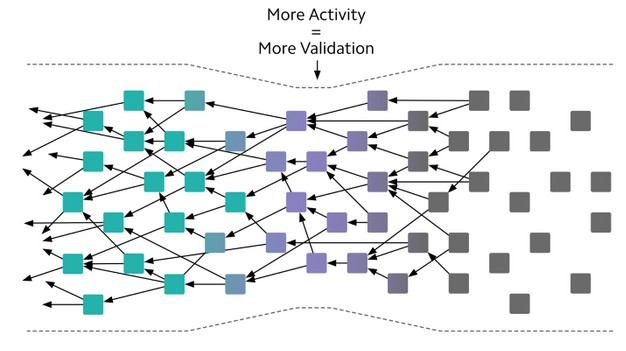
\includegraphics[width=0.8\linewidth]{Figures/Selection_039.jpg}}
\caption{Funcionamiento del Tangle de \cite{tangle_picture}.}
\label{fig:Selection_039}
\end{figure}

\begin{itemize}
\item \textbf{Cuentas} \newline
A diferencia de otras criptomonedas, IOTA no usa un conjunto de clave pública con clave privada para definir una cuenta. Cada usuario posee una semilla, que es un número aleatorio y secreto. Con la semilla se crea una clave pública y una clave privada. La clave pública es usada como destino para fondos. Si el usuario desea gastar los fondos asociados a dicha clave, firma la transferencia con la clave privada correspondiente. Luego, el conjunto de clave pública y privada es descartado y se genera uno nuevo con la semilla secreta. Ese mecanismo se llama esquema de firma única, ya que cada transacción es firmada con una única clave que no se reutiliza.

\item \textbf{Validación} \newline
Para transferir tokens IOTA de una cuenta a otra, hay que seguir los siguientes pasos:
\begin{enumerate}
\item La transacción tiene que ser firmada con claves que todavía no han sido utilizadas.
\item Es necesario elegir y validar dos \textit{tips}: \textit{Tips} son transacciones cuya historia todavía no fue comprobada y se verifica que no existen contradicciones entre ambas transacciones.
\item Se calcula un \textit{Proof of Work} para cada transacción que se publica. De esa forma se evita \textit{spam} en la red.
\end{enumerate}
Luego de completar los pasos descritos, la transacción nueva es publicada como \textit{tip} y otros nodos pueden elegirla para la validación. 

\item \textbf{Costo de transacciones} \newline
Ya que no existen mineros ni forjadores, tampoco existen tarifas de transacciones. El costo de una transacción consiste en el esfuerzo computacional que requiere validar dos \textit{tips} y calcular el \textit{Proof of Work}.
\end{itemize}

IOTA resulta ser una implementación prometedora ya que desafía la arquitectura tradicional del Blockchain e introduce mayores cambios en su funcionamiento. Todavía se encuentra en las etapas tempranas de desarrollo y queda por ver si las mejoras introducidas producen el impacto esperado.


Para la aplicación a implementar, la arquitectura de IOTA presenta los siguientes inconvenientes:

\begin{itemize}
\item El esquema de firma única no permite asignar una identidad única a los participantes de la red.
\item La solución ``Qubic'' para que IOTA soporte \textit{smart contracts} todavía está en desarrollo y no existe una fecha estimativa de lanzamiento. \cite{qubic_roadmap}
\end{itemize}


\section{Lisk}

Lisk es un producto de la Lisk Foundation: CEO Max Kordek y CTO Oliver Beddows quieren implementar un \textit{framework} que ayuda con la creación de Blockchains nuevos - públicos o privados - para una adaptación más simple y rápida de la tecnología.
En mayo del 2016, se lanzó su Blockchain que actualmente permite el intercambio de la criptomoneda LSK y la implementación de aplicaciones descentralizadas, parecido al caso de Ethereum y EOSio. El \textit{framework} que facilita la construcción de un Blockchain propio está en versión alpha y todavía se encuentra en desarrollo.

\subsection{Funcionamiento}

\begin{itemize}

\item \textbf{Cuentas}\newline
Para poder empezar a interactuar con la red de Lisk, es necesario instalar Lisk Hub.
\begin{quote}
Lisk Hub es una solución todo en uno para administrar el ID de Lisk, acceder a los tokens de Lisk, enviarlos así como también para votar a los delegados. Combina la funcionalidad de la antigua billetera y un explorador de Blockchain.\cite{lisk_products}
\end{quote}
A partir de una frase de contraseña secreta se genera un Lisk-Id, un identificador único de la cuenta de usuario. Con dicho Lisk-Id es posible recibir y transferir fondos. Las transacciones tienen que ser firmadas con la frase de contraseña secreta para ser procesadas.

\item \textbf{Validación} \newline
Lisk utiliza \textit{delegated proof of stake} para forjar bloques nuevos.\cite{lisk_consensus} Existen 101 delegados que crean bloques en turno rotatorio y se genera un bloque nuevo cada 10 segundos. Cada bloque incluye 25 transacciones, de modo que Lisk tiene un rendimiento de 2,5 transacciones por segundo. Los delegados cobran un monto de 5 LSK por cada bloque creado y adicionalmente una tarifa por cada transacción incluida en el bloque. Los participantes de la red deben votar a los delegados y pueden recibir un porcentaje de la ganancia del delegado como incentivo de voto.

\item \textbf{Costo de transacciones} \newline
Las transacciones en la red Lisk tienen un costo fijo de 0,1LSK, sin importar el monto que se está transfiriendo.\cite{lisk_transactions} Existe una propuesta para la implementación de tarifas dinámicas pero todavía no se encuentra considerada en el \textit{roadmap} de la implementación. 

\end{itemize}

Para utilizar el \textit{framework}, los futuros implementadores Blockchain pueden descargar las herramientas Lisk Commander, Lisk Core y Lisk Elements, que forma un conjunto de librerías y herramientas que permiten configurar parámetros de un Blockchain propio. El lenguaje principal es Javascript, de esa manera, programadores que provienen de un ambiente de desarrollo web pueden empezar a trabajar con Lisk sin tener que aprender un lenguaje nuevo. Será posible ajustar el mecanismo de consenso, tarifas de transacciones, derechos de accesos, rendimiento como también codificar la aplicación.

Sin embargo, no es la visión de la fundación Lisk que en un futuro haya una multitud de Blockchains aislados entre sí: su objetivo es la interacción entre ``Sidechains''.

 
Sidechains fueron descritos por primera vez en el whitepaper ``Enabling Blockchain Innovations with pegged Sidechains'' donde los autores definen el concepto de la forma siguiente:

\begin{quote}
Proponemos una nueva tecnología, los Sidechains vinculados, que permite transferir Bitcoins y otros activos contables entre múltiples Blockchains.\cite{Back2014EnablingBI}
\end{quote}

Así, un Sidechain es un Blockchain que implementó un mecanismo para poder intercambiar activos con otros Blockchains. Construir aplicaciones en Sidechains tiene varias ventajas:
\begin{enumerate}
\item Es posible definir el mecanismo de consenso y forjado más conveniente para una aplicación.
\item Problemas como errores de código o ataques solamente afectan a un Sidechain.
\item Bienes pueden ser intercambiados entre diferentes Sidechains sin ser convertidos: un Bitcoin en un Sidechain sigue siendo un Bitcoin.
\end{enumerate}

Max Kordek describe su idea para los Sidechains de Lisk de la siguiente manera: 
\begin{quote}
Es posible usar las funcionalidades del Sidechain de otras personas dentro de un Sidechain propio. Por ejemplo, si hay un servicio para enviar mensajes y otro que permite subir imágenes, se pueden aprovechar estas dos aplicaciones para construir una aplicación como una red social, sin volver a implementar la subida de imágenes y el servicio de mensajería. Simplemente se usan otras aplicaciones de Blockchain para eso. Es como un cerebro que evoluciona con cada Sidechain que está conectada al sistema.\cite{youtube_lisk}
\end{quote}

Según el CEO del proyecto, una vez que el \textit{framework} está implementado, será posible implementar un Blockchain privado, adaptar parámetros como costos de transacción y el mecanismo de consenso, e implementar la aplicación que funcione con dicho Blockchain. El \textit{framework} tendría la ventaja para los desarrolladores que mientras ellos se pueden concentrar en escribir la aplicación, Lisk se encargaría de mejorar el funcionamiento de la tecnología Blockchain subyacente. El proyecto tiene aspectos prometedores para el futuro y si su desarrollo estuviese más avanzado, sería considerado como una opción para este proyecto integrador, ya que cumple con los requisitos establecidos.


\section{Hyperledger}

Hyperledger es un proyecto de la Linux Foundation que fue iniciado en diciembre de 2015.
\begin{quote}
El proyecto va a desarrollar un \textit{framework} de código abierto y grado empresarial para \textit{ledgers} distribuidos, con el fin de que desarrolladores se enfoquen en construir aplicaciones robustas y específicas de su industria.\cite{hyperledger_foundation}
\end{quote} 
Los términos \textit{ledger} y Blockchain en este contexto describen el mismo concepto, y más adelante se va a aclarar la diferencia entre ambos.

Una variedad de empresas apoya la iniciativa: en septiembre de 2018 figuran más que 250 miembros en la página web, entre otros Cisco, Hitachi y J.P.Morgan. IBM e Intel aportaron código de trabajos relacionados con Blockchain, lo cual formó la base para los dos proyectos más avanzados: Hyperledger Fabric y Hyperledger Sawtooth.

Desde los inicios de Hyperledger se sumaron una multitud de proyectos. En total hay 5 \textit{frameworks} para diferentes tipos de Blockchains y 5 herramientas que facilitan la interacción y el mantenimiento. En la figura \ref{fig:Selection_051} se ve el enfoque de cada uno.
\begin{figure}[H] % Example image
\center{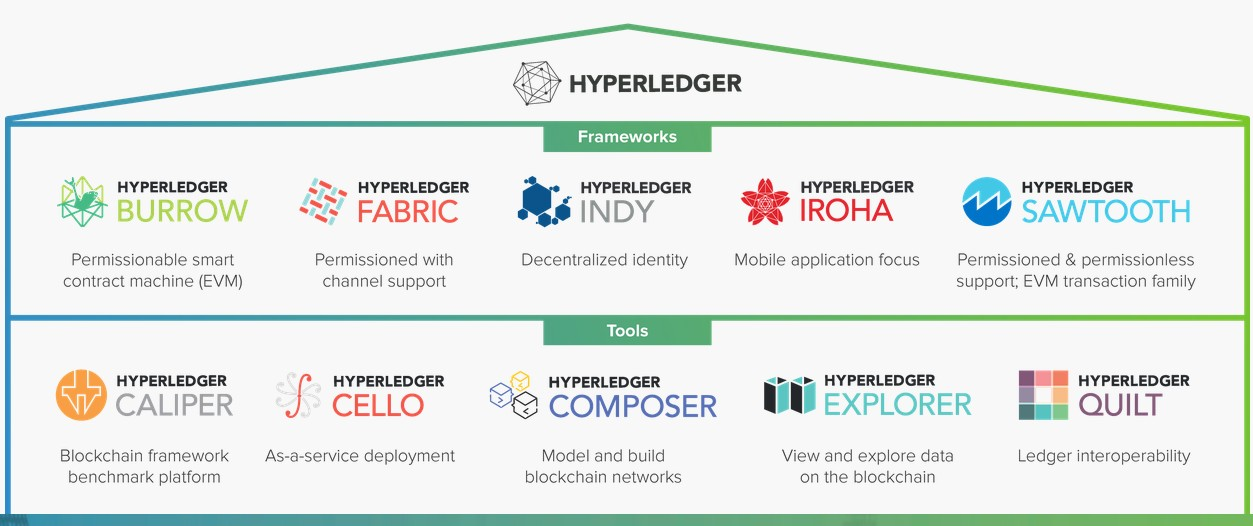
\includegraphics[width=1.0\linewidth]{Figures/Selection_051.jpg}}
\caption{Proyectos en Hyperledger de \cite{hl-projects}.}
\label{fig:Selection_051}
\end{figure}

La mayoría de los proyectos que figuran en \ref{fig:Selection_051} se encuentran en la etapa de incubación, por lo cual su código y su documentación se encuentran incompletos. A continuación se van a describir con mayor detalle los dos proyectos más avanzados, que cuentan con una versión 1.0 y pueden ser usados en producción.

\subsection{Hyperledger Fabric}
Hyperledger Fabric fue el primero de los proyectos Hyperledger y su versión 1.0 se lanzó el 11.7.2017.\cite{hlf_release} Es un \textit{framework} para implementar Blockchains de uso empresarial. Fue diseñado con los siguientes requerimientos:\cite{hlf_whatis}
\begin{itemize}
\item[\textendash] Los participantes tienen que ser identificables.
\item[\textendash] El acceso a la red debe ser autorizado.
\item[\textendash] El sistema necesita alto rendimiento para procesar transacciones.
\item[\textendash] Las transacciones se tienen que confirmar con baja latencia.
\item[\textendash] El sistema debe proveer privacidad y confidencialidad para las transacciones y sus datos relacionados.
\end{itemize}

Los requerimientos especificados se implementaron de la siguiente manera:
\begin{itemize}
\item \textbf{Cuentas} \newline
Organizaciones que participan en el Blockchain hacen uso de una autoridad de certificación - puede ser propia o tercera - para otorgar identidades digitales a sus usuarios. Hyperledger Fabric cuenta con un \textit{Membership Service Provider} y listas de control de acceso: cada identidad digital es verificada con respecto a su validez y sus autorizaciones cuando se conecta a la red.
\item \textbf{Validación} \newline
En Hyperledger Fabric, los nodos que validan transacciones no son los mismos que los nodos que crean bloques nuevos. Así, la carga de procesamiento en la red se distribuye mejor. Además, la división permite la ejecución paralela de transacciones no relacionadas, mejorando así el rendimiento del Blockchain.

\item \textbf{Costo de Transacciones} \newline
Si bien es posible definir una criptomoneda nativa en Hyperledger Fabric, no es necesario y el protocolo de consenso no lo requiere.
\begin{quote}
Fabric puede utilizar protocolos de consenso que no requieren de una criptomoneda nativa para incentivar el minado costoso o para impulsar la ejecución de \textit{smart contracts}.\cite{hlf_whatis}
\end{quote}
 Por ende, las transacciones pueden ser ejecutadas sin pagar una tarifa.
\end{itemize}

\subsection{Hyperledger Sawtooth}
El 30.1.2018, Hyperledger lanzó la versión 1.0 de un segundo proyecto llamado Hyperledger Sawtooth.\cite{hls_release} El código inicial fue aportado por Intel y fue diseñado con los siguientes objetivos:\cite{hls_whatis}
\begin{itemize}
\item[\textendash] Construir una plataforma para \textit{ledgers} distribuidos que sean privados o públicos.
\item[\textendash] Lograr una configuración fina de permisos de accesos y transacciones.
\item[\textendash] Asegurar que \textit{smart contracts} sean seguros.
\item[\textendash] Obtener una separación estricta de la lógica de negocios con la implementación subyacente y facilitar así el desarrollo.
\end{itemize}

El software funciona de la forma siguiente:
\begin{itemize}
\item \textbf{Cuentas}\newline
Con la ayuda de identidades criptográficas se crean roles con determinados permisos. Los clientes interactúan a través de una REST-API con una red de validadores, que verifican los permisos de los clientes y rechazan peticiones si los permisos no son suficientes. Si la petición de una transacción se considera válida, se la envía a un nodo procesador de transacciones para su ejecución. Dichos nodos son los que actualizan el estado del Blockchain.
\item \textbf{Validación} \newline
Como en Hyperledger Fabric, la validación de transacciones y la creación de bloques ocurren en nodos diferentes. Hyperledger Sawtooth ofrece un mecanismo de consenso nuevo llamado \textit{Proof of Elapsed Time}, que aprovecha un ambiente seguro de ejecución en los procesadores Intel. Sin embargo, una característica de Hyperledger Sawtooth es el ``mecanismo de consenso intercambiable'': La forma de llegar al consenso puede ser cambiada por una alternativa proponiendo un cambio a través de una transacción.
\item \textbf{Costo de Transacciones} \newline
Al igual que en Hyperledger Fabric, Hyperledger Sawtooth no  requiere de una criptomoneda para asegurar transacciones y consenso, por lo cual el costo de las transacciones se reduce al costo de procesamiento en la red que requiere cada transacción.
\end{itemize}


Junto con los ya mencionados, Hyperledger Sawtooth provee una cantidad de mecanismos adicionales que distinguen la implementación de Hyperledger Fabric.

Las transacciones se pueden enviar en lotes: se deben ejecutar todas las transacciones de forma exitosa o ninguna. Así se consigue implementar transacciones atómicas como en  bases de datos tradicionales.

Los nodos procesadores de transacciones son capaces de aprovechar paralelismo de transacciones no relacionados, mejorando así el rendimiento del Blockchain.

Hyperledger Sawtooth es compatible con Solidity, es decir \textit{smart contracts} escritos para Ethereum pueden ser ejecutados en Hyperledger Sawtooth con la ayuda de la herramienta Seth. Además, pueden ser testeados en \textit{sandboxes}, ambientes seguros para evitar comportamientos inesperados.

La configuración del Blockchain está guardada en forma de transacciones en el mismo Blockchain, lo cual tiene la ventaja que nodos que son agregados adicionalmente se pueden auto configurar. Además, posibilita modificar el funcionamiento de un Blockchain que ya está en uso: se proponen cambios en forma de transacciones que son aprobados o rechazados en base a un sistema de votos integrado en Hyperledger Sawtooth.


\subsection{Otros proyectos de Hyperledger}

\textbf{Hyperledger Iroha}: Una implementación con un esquema de consenso nuevo que es de alta performance y orientado a dispositivos móviles que se conectan y desconectan con frecuencia de la red. El proyecto todavía está en la versión beta.


\textbf{Hyperledger Burrow}: Es un cliente Blockchain con la máquina virtual de Ethereum integrada. Está diseñado para ejecutar \textit{smart contracts} escritos en Solidity y, para ser usado en un ambiente donde diferentes Blockchains están conectadas entre ellos. Se encuentra en la etapa de incubación. 

\textbf{Hyperledger Indy}: Un \textit{framework} para un Blockchain diseñado para la gestión de identidades digitales. Como Hyperledger Burrow, está en la etapa de incubación.

Otros productos de Hyperledger están pensados para facilitar el desarrollo, como por ejemplo \textbf{Hyperledger Cello}, una herramienta para el despliegue en \textit{clusters} con el fin de ofrecer Blockchain como servicio. \textbf{Hyperledger Caliper} permite realizar \textit{benchmarks} de Blockchains e \textbf{Hyperledger Explorer} posibilita administrar a un Blockchain a través de una interfaz web. Todas las herramientas de Hyperledger se encuentran en etapa de incubación.

Los dos proyectos que se detallaron en esta sección cuentan con las características especificadas para el prototipo. \ref{sec:primeras_especificaciones_prototipo}. Son \textit{frameworks} completamente desarrollados que permiten implementar un Blockchain con las funcionalidades requeridas. De los dos, Hyperledger Fabric se destaca como la opción más conveniente debido a que está específicamente destinado a Blockchains privados y para el prototipo a emplear no se necesita la compatibilidad con Ethereum. Además, emplear \textit{Proof of Elapsed Time} implica una limitación con respecto al \textit{hardware}, ya que el algoritmo solamente funciona en conjunto con arquitectura Intel, por lo cual la mecánica de consenso de Hyperledger Fabric resulta más adecuada.

\section{Conclusiones}
En el mercado existen muchas soluciones para implementar aplicaciones en Blockchain, algunas más desarrolladas que otras. Cada solución tiene su propio enfoque y en el momento de la redacción del informe, la mayoría requieren de un medio de pago en forma criptomonedas. Sin embargo, el código de dichas plataformas suele ser libre y \textit{open source}, por lo cual un equipo de programadores experimentados puede implementar un Blockchain propio haciendo las modificaciones deseadas en un código ya existente.

Para un despliegue de mayor velocidad con un \textit{framework} ya existente, se ofrecen las soluciones de Hyperledger, donde especialmente Hyperledger Fabric e Hyperledger Sawtooth cuentan con un código testeado para ser empleado en ambientes de producción, el soporte de varios lenguajes de programación para aplicaciones y una amplia cantidad de documentación con tutoriales.

Hyperledger Fabric es una solución de código libre que cumple con las siguientes caracterísiticas:

\begin{itemize}
    \item Es una solución pensada para Blockchains privados y Blockchains de Consorcio.
    \item Los permisos de acceso son configurables a través de identidades digitales, que también permiten la implementación de una lista negra para casos de identidades perdidas o robadas. En cada momento, es posible controlar los accesos de lectura y escritura de cualquier entidad.
    \item Si bien el uso de una criptomoneda es posible, el protocolo de consenso no requiere de un incentivo en forma de una criptomoneda.
    \item Los \textit{smart contracts} son fácilmente programables en el lenguaje de programación Golang.
\end{itemize}

Dado que las características mencionadas cumplen con los requerimientos planteados para una solución Blockchain, elaborados en la sección \ref{sec:primeras_especificaciones_prototipo}, se eligió Hyperledger Fabric como \textit{framework} para la implementación del prototipo.

\newpage 
% % Chapter 3

\chapter{Hyperledger Fabric} % Main chapter title

\label{Chapter3} % For referencing the chapter elsewhere, use \ref{Chapter1} 

\lhead{Capítulo 3. \emph{Hyperledger Fabric}} % This is for the header on each page - perhaps a shortened title
\setstretch{1.1} % Line spacing of 1.1
Para poder proceder con el diseño de un prototipo resulta necesario conocer los detalles de la implementación de la plataforma elegida. Por eso, el objetivo del presente capítulo es adquirir un profundo conocimiento de terminología, diseño y funcionamiento de Hyperledger Fabric.

%----------------------------------------------------------------------------------------
%	SECTION 1
%----------------------------------------------------------------------------------------

\section{Composición de la red Blockchain}
\label{composicion_red_blockchain}
%explicacion de peers y ledger
Como también en otras implementaciones ya estudiadas, la red se compone por un conjunto de nodos participantes o \textit{peers}, que intercambian mensajes sobre el estado del Blockchain. \textit{Peers} son los elementos más fundamentales de Hyperledger Fabric, ya que almacenan el \textit{ledger}, o el Blockchain.
Los términos \textit{ledger} o Blockchain este contexto describen el mismo concepto y se van a utilizar ambos términos de forma intercambiable, hasta aclarar la diferencia en la sección \ref{sec:ledger_and_world_state}.
%explicación de chaincode
Además, los \textit{peers} ejecutan los \textit{smart contracts}, que en Hyperldeger Fabric se llaman \textit{chaincodes}. Existen dos operaciones sobre el Blockchain: la de lectura y la de escritura. Ambas operaciones tienen que ser implementadas en el \textit
{chaincode}: la existencia de una instancia del \textit{ledger} solo no permite leer o modificar información.

Una colección de \textit{peers} cumple con las siguientes características:
\begin{itemize}
    \item Cada \textit{peer} que pertenece a la red, almacena una instancia del \textit{ledger} y una instancia del \textit{chaincode}.
    \item Al existir instancias iguales en todos los nodos, se evita un único punto de fallo: Cuando el \textit{ledger} es modificado, cada \textit{peer} actualiza su instancia.
    \item Ya que cada \textit{peer} es capaz que acceder y modificar el Blockchain, una aplicación que necesita leer o modificar el \textit{ledger}, lo tiene que hacer a través del \textit{peer}.
    \begin{figure}[H] % Example image
        \center{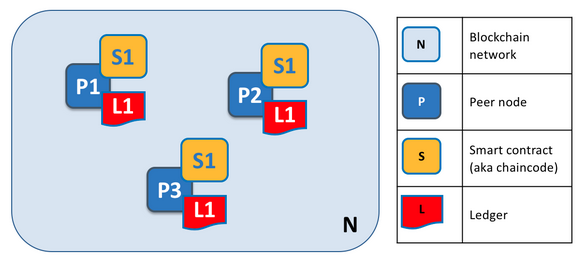
\includegraphics[width=1.0\linewidth]{Figures/Selection_169.png}}
        \caption{Una red Blockchain con 3 \textit{peers}: Cada \textit{peer} corre una instancia idéntica del \textit{chaincode} y del \textit{ledger}. De \cite{hlf-peers}.}
        \label{fig:Selection_169}
    \end{figure}  
    
\end{itemize}
La figura \ref{fig:Selection_169} ilustra lo descrito: En una red se encuentran 3 \textit{peers}, donde cada uno tiene una copia del \textit{ledger} y del \textit{chaincode}. \textit{Peers} pueden ser agregados o eliminados de la red de forma dinámica, según las necesidades de los administradores. No existen limitaciones con respecto a la cantidad de \textit{peers} que pueden conformar una red.

\section{La existencia de varios \textit{ledgers}}
En la sección anterior se explicó que cada \textit{peer} almacena su instancia del \textit{ledger} y del \textit{chaincode} y que los datos pueden ser actualizados solamente a través del \textit{chaincode}. Una analogía sería permitir la lectura y escritura de una base de datos relacional solamente a través de llamadas a una API, en vez de ejecutar instrucciones SQL directamente.

Una particularidad de Hyperledger Fabric consiste en posibilitar la existencia de varios \textit{ledgers}: Un \textit{peer} puede almacenar diferentes Blockchains como también diferentes \textit{chaincodes} que acceden al Blockchain correspondiente. La figura \ref{fig:Selection_170} visualiza la situación descrita: El \textit{peer} P1 aloja \textit{ledger} L1, al cual puede acceder con los \textit{chaincodes} S1 y S2. A su vez, aloja \textit{ledger} L2, accesible a través de S1 y S3.

\begin{figure}[H] % Example image
    \center{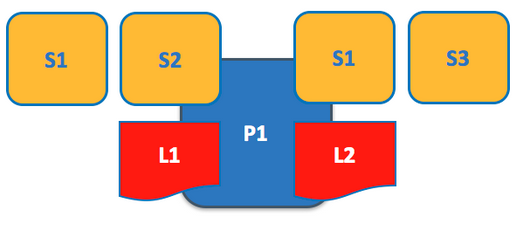
\includegraphics[width=0.7\linewidth]{Figures/Selection_170.png}}
    \caption{Un peer que aloja 2 \textit{ledgers} y 3 diferentes \textit{chaincodes}. De \cite{hlf-peers}.}
    \label{fig:Selection_170}
\end{figure}

No existen límites con respecto a esa arquitectura: un peer puede alojar tantos \textit{ledgers} y \textit{chaincodes} como se desea. Tampoco hay una relación requerida entre la cantidad de \textit{ledgers} y \textit{chaincode}: un peer teóricamente puede alojar un \textit{ledger} sin \textit{chaincode} que acceda a él. Cada \textit{ledger} almacena información independientemente de otros \textit{ledgers} y funciona como un Blockchain diferente.

En un ambiente de Blockchains privados, el paradigma descrito es de mucha utilidad: Un conjunto de empresas puede decidir compartir información en un \textit{ledger} al cual acceden todos los participantes, pero también pueden existir \textit{ledgers} entre un subconjunto de participantes, permitiendo un grado de privacidad mayor. En la figura \ref{fig:ledgers} se muestra el escenario descrito.

\begin{figure}[H] % Example image
    \center{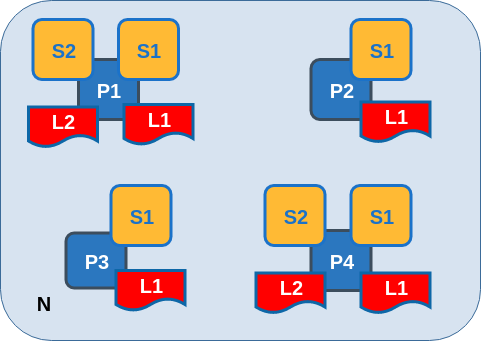
\includegraphics[width=0.7\linewidth]{Figures/ledgers.png}}
    \caption{Una red con 2 \textit{ledgers} diferentes: \textit{peers}  P2 y P3 no saben de la existencia del \textit{ledger} L2, sin embargo, todos los \textit{peers}  comparten información en el \textit{ledger} L1. }
    \label{fig:ledgers}
\end{figure}

Recordando las implementaciones analizadas en el capítulo \ref{Chapter2}, por cada red de participantes existía un sólo Blockchain que almacenaba todas las transacciones efectuadas de la red: La arquitectura de Hyperledger Fabric permite mantener una multitud de Blockchains en una misma red, donde los \textit{peers}  solamente tienen conocimiento de los \textit{ledgers}  que alojan.

\section{Aplicaciones y la red Blockchain}
\label{sec:aplicaciones_y_redBC}

Como se mencionó en la sección \ref{composicion_red_blockchain}, es necesario que aplicaciones accedan al Blockchain estableciendo una conexión con los \textit{peers}. Para lograr eso, Hyperledger Fabric provee SDKs en los lenguajes Java, Python, Go y Nodejs. Programadores pueden utilizar las funciones del SDK para conectarse a la API expuesta por cada \textit{peer} e invocar \textit{chaincode}.

Una aplicación se puede conectar a un \textit{peer} para consultar información existente en el Blockchain o para actualizar su estado. El flujo de cada una de las operaciones se ve detallado en la figura \ref{fig:transaction_flow}.

Para el caso de una consulta se requieren 3 pasos:
\begin{enumerate}
    \item La aplicación se conecta al \textit{peer} correspondiente. Qué aplicación se conecta a qué \textit{peer} de la red es indiferente, siempre y cuando el \textit{peer} tenga conocimiento del \textit{ledger} y \textit{chaincode} que se está por acceder.
    \item Luego de una conexión exitosa, la aplicación envía una propuesta al \textit{peer}, que invoca el \textit{chaincode} correspondiente.
    \item El \textit{peer} espera la respuesta del \textit{chaincode} invocado y la retorna al \textit{peer}.
\end{enumerate}
Como el peer mantiene una instancia completa y actualizada del \textit{ledger} y del \textit{chaincode}, no es necesario que verifique sus resultados con otros participantes de la red: puede satisfacer la consulta solo y de forma inmediata. La característica descrita garantiza la alta disponibilidad del Blockchain: La carga de muchas operaciones de lectura puede ser distribuida entre una multitud de \textit{peers} y la caída de un \textit{peer} no afecta la disponibilidad de la información.

\begin{figure}[H] % Example image
    \center{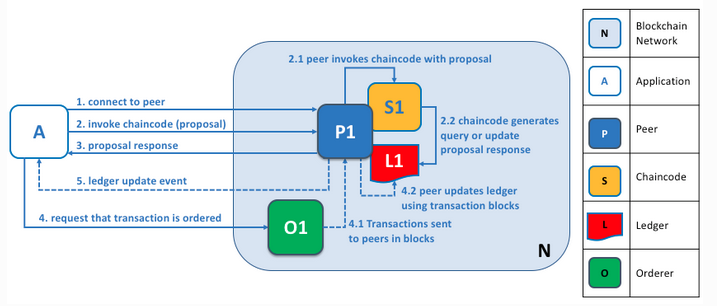
\includegraphics[width=1.0\linewidth]{Figures/Selection_171.png}}
    \caption{Flujos de consulta y actualización del \textit{ledger}. De \cite{hlf-peers}. }
    \label{fig:transaction_flow}
\end{figure}

Una actualización del \textit{ledger} requiere el consenso de una multitud de \textit{peers}, por lo cual se requieren más pasos:
\begin{enumerate}
    \item Cada \textit{chaincode} posee su propia política de aprobación que especifica cuantos \textit{peers}  tienen que aprobar la transacción para que ésta puede ser agregada al Blockchain. Cuando una aplicación quiere escribir datos o cambios, envía una propuesta a todos los \textit{peers}  necesarios para que la transacción pueda ser aprobada.
    \item Cada \textit{peer} determina que la propuesta sea válida, que la misma propuesta no se ha hecho anteriormente (protección contra un ataques de repetición) y que la aplicación tenga los permisos suficientes para realizar una escritura en el \textit{ledger}. Si se cumplen todas las condiciones, el \textit{chaincode} es ejecutado por todos los \textit{peers}  que lo recibieron y los resultados se envían en forma de una respuesta a la aplicación. Es importante entender que en el momento que la aplicación recibe las respuestas, todavía no se cambió el estado del Blockchain.
    \item La aplicación recibe las respuestas, verifica que todas sean iguales y si es el caso, manda su propuesta junto con las respuestas obtenidas al ``servicio para ordenar transacciones'' (\textit{ordering service}) para que la transacción sea agregada al \textit{ledger}.  
    \item Un \textit{peer} especial llamado \textit{orderer} cumple con la función de recibir diferentes transacciones, ordenarlas cronológicamente en bloques de datos y publicarlas en la red. 
    \item Una vez que se emitió el bloque nuevo a todos los \textit{peers}  suscritos al \textit{ledger} correspondiente, los \textit{peers}  verifican que la transacción en sí es válida y que se cumplió con la política de aprobación requerida. Luego, la transacción se declara como válida o inválida.
    \item Al completar el proceso descrito, la aplicación cliente es informada sobre la validez de la transacción y sobre su inclusión en el Blockchain. Debido al procesamiento requerido, la respuesta puede demorar varios segundos.
\end{enumerate} 

Vale aclarar que una ``actualización'' en este contexto no sobre escribe valores existentes: como en todas las implementaciones Blockchain, el \textit{ledger} es inmutable y no soporta operaciones de borrado o sobre escritura. ``Actualizar'' al Blockchain entonces significa simplemente agregar información nueva.

\section{Canales}
En la sección anterior, se explicó que un bloque nuevo es emitido a todos los \textit{peers}  suscritos a un \textit{ledger}. A continuación se va a explicar cómo funciona dicha subscripción. En Hyperldeger Fabric se usa un concepto llamado ``canales''.

Un canal describe un conjunto de \textit{peers}, un servicio de pedidos y un \textit{ledger} con su respectivo \textit{chaincode}. Todos los \textit{peers}, los nodos que se encargan del servicio de pedidos y las aplicaciones que se unen a un canal van a tener acceso a copias idénticas del mismo \textit{ledger}. Así, para que puedan existir varios \textit{ledgers} diferentes en una red, tienen que existir varios canales y los participantes que quieren acceder a los \textit{ledgers} en cuestión tienen que formar parte del canal correspondiente.

\begin{figure}[H] % Example image
\center{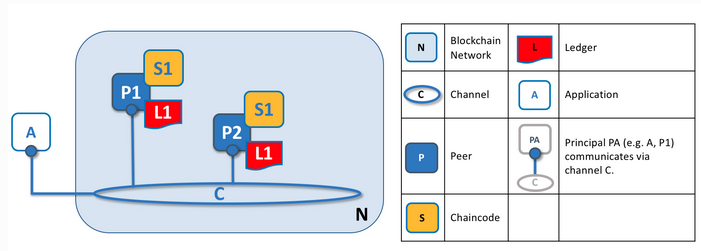
\includegraphics[width=1.0\linewidth]{Figures/Selection_172.png}}
\caption{Visualización del concepto de canal. De \cite{hlf-peers}.}
\label{fig:channels}
\end{figure}


\section{Agrupación de la red en organizaciones}

Tal como en Hyperledger Fabric se agrupan en canales los miembros de la red que acceden a un mismo \textit{ledger}, también se agrupan los \textit{peers}  según la organización a la que pertenecen.

El concepto de organización en Hyperledger Fabric describe una entidad que participa en la red y que conecta sus \textit{peers} a ella. La idea es que equivale a una organización en el mundo real: En el contexto del proyecto integrador, las organizaciones podrían ser las diferentes facultades que comparten información en una red Blockchain de la UNC.

Una organización puede aportar tantos \textit{peers}  a la red como desea. En la figura \ref{fig:organizations} la red está conformada por cuatro organizaciones y cada una tiene como mínimo un \textit{peer} conectado a un canal en común. También se puede observar que cada organización tiene su propia aplicación para acceder a los \textit{peers}: El desacoplado entre aplicación de usuario y \textit{chaincode} permite la implementación de una multitud de aplicaciones que consumen los datos compartidos de un mismo Blockchain.

\begin{figure}[H] % Example image
    \center{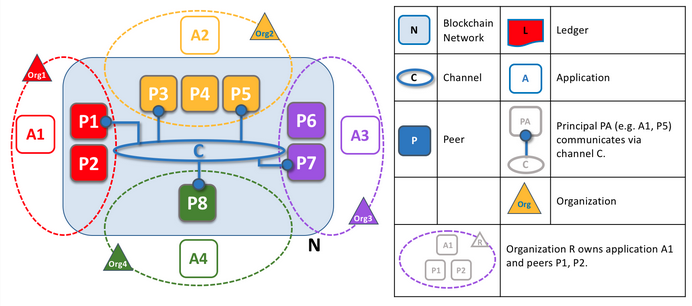
\includegraphics[width=1.0\linewidth]{Figures/Selection_173.png}}
    \caption{Una red Blockchain conformada por 4 organizaciones.}
    \label{fig:organizations}
\end{figure}

\section{La Identidad de los \textit{peers} en la red Blockchain}
\label{sec:identidad_de_peers}
¿Cómo reconoce la red qué \textit{peer} pertenece a qué organización? En Hyperledger Fabric, cada organización administra su propia Autoridad de Certificación (CA por sus siglas en inglés), que provee una identidad digital en forma de un certificado X.509 para cada \textit{peer} que se une a la red. La figura \ref{fig:identidad} describe un esquema de dos organizaciones con sus autoridades de certificación correspondientes.

Pero los certificados no solamente son para \textit{peers}: cualquier entidad que se quiere conectar a la red, también las aplicaciones, necesitan una identidad digital autorizada, sino su conexión será rechazada.

Si bien un \textit{peer} puede tener acceso a varios \textit{ledgers} compartidos entre diferentes organizaciones, siempre pertenece a una sola organización, la cual se determina con su identidad digital. Un \textit{peer} no puede ser compartido entre múltiples organizaciones.

\begin{figure}[H]
    \center{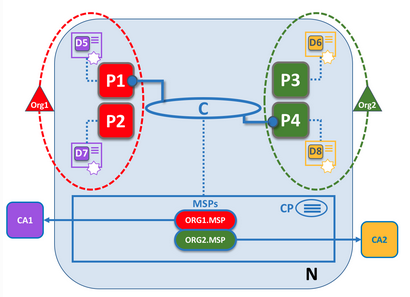
\includegraphics[width=0.7\linewidth]{Figures/Selection_176.png}}
    \caption{Una red compuesta de dos organizaciones, sus respectivas autoridades de certificación y sus MSP. Cada \textit{peer} tiene una identidad digital asociada, \textit{peer} P1 por ejemplo se identifica en el canal con la identidad D5. De \cite{hlf-peers}.}
    \label{fig:identidad}
\end{figure}

Los flujos de autenticación y autorización en Hyperledger Fabric son manejados por un \textit{Membership Service Provider} o MSP. Éste trabaja a dos niveles:
\begin{itemize}
    \item El \textit{Membership Service Provider} a nivel de canal identifica a qué organización pertenece cada \textit{
    peer} y controla que la participación y la administración del Blockchain solamente puede realizarse por los \textit{peers}  con los derechos correspondientes.
    \item El \textit{Membership Service Provider} a nivel local está funcionando adentro de cada \textit{peer}: Su objetivo es verificar los derechos de acceso de lectura y escritura de los clientes o aplicaciones que se conectan a él con el objetivo de invocar \textit{chaincode}. 
\end{itemize}

La comunicación entre los diferentes \textit{peers}  funciona a través de un protocolo \textit{gossip}, pero para que todos los participantes de un canal empiecen a compartir información, es necesario que cada miembro tenga conocimiento de los demás miembros de la red. Para el descubrimiento de \textit{peers}  en un canal se define un mínimo de un \textit{anchor peer} por canal: \textit{peers}  de todas las organizaciones notifican al \textit{anchor peer} sobre los miembros que pertenecen a su organización y reciben información sobre otros \textit{peers}  de otras organizaciones como respuesta. Luego de la etapa de descubrimiento, todos los \textit{peers}  del canal pueden comunicarse entre ellos y el \textit{anchor peer} solamente se va a volver a necesitar cuando se agreguen nodos a la red o se apagan. Se recomienda que cada organización tenga su conjunto de \textit{anchor peers} así se evita un único punto de fallos.

\section{Los \textit{Ledgers} y el \textit{World State}} \label{sec:ledger_and_world_state}
En la presente sección, se van a definir con mayor detalle los términos Blockchain y \textit{ledger} bajo el contexto de Hyperledger Fabric.

\textit{Ledger} es un término del inglés cuya traducción directa es ``libro contable''. Describe un registro que contiene el estado actual de un negocio junto con un historial de transacciones que llevaron a dicho estado.

En un \textit{ledger} se almacenan datos respecto a un cierto negocio. Los datos se pueden ver como objetos del negocio, aunque solamente son abstracciones de dichos objetos. En el caso de uso presentado, un objeto sería un acta de una facultad y el estado del acta puede cambiar de válido a inválido en el caso de ser revocado.

En Hyperledger Fabric, el registro histórico que lleva al estado actual es el Blockchain. Está estructurado como un registro secuencial de bloques interconectados, donde cada bloque contiene una secuencia de transacciones, cada transacción representa una consulta o actualización del estado de los objetos almacenados. La figura \ref{fig:bc_hlf} representa la estructura en forma gráfica: se puede observar que no existen diferencias fundamentales con otras implementaciones como Bitcoin.

\begin{figure}[H]
    \center{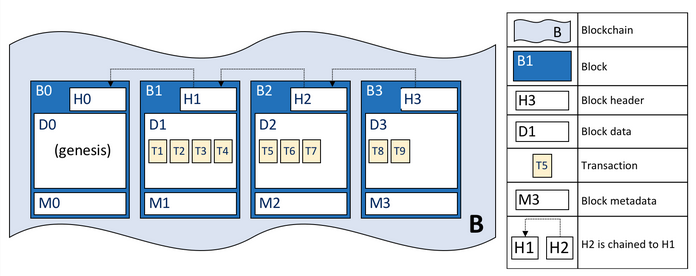
\includegraphics[width=0.8\linewidth]{Figures/Selection_186.png}}
    \caption{La estructura del Blockchain en Hyperledger Fabric. De \cite{hlf-ledger}.}
    \label{fig:bc_hlf}
\end{figure}

El Blockchain se almacena como un solo archivo y la operación más frecuente que se efectúa sobre éste es adjuntar bloques adicionales. Como el archivo no se encuentra indexado, consultas sobre el estado actual implican iterar de forma secuencial sobre los bloques almacenados, lo cual resulta ineficiente. Para resolver ese problema, Hyperledger Fabric extrae el estado actual del Blockchain y lo guarda en una base de datos. El conjunto de los estados actuales de todos los objetos lleva el nombre \textit{world state}.

Para el \textit{world state}, Hyperledger Fabric ofrece dos opciones de base de datos diferentes: La primera es LevelDB, un simple almacenamiento para datos en el formato clave-valor. Para almacenar objetos JSON con mayor complejidad, se recomienda CouchDB. Consultas en CouchDB se pueden hacer sobre claves y valores, no solamente sobre claves como en LevelDB. Además, CouchDB permite actualizar solamente partes del objeto JSON, mientras en LevelDB la actualización afecta al objeto entero.

\begin{figure}[H]
    \center{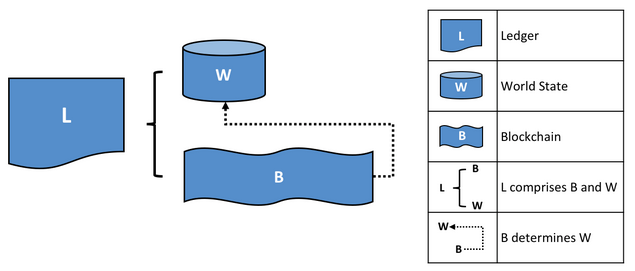
\includegraphics[width=0.8\linewidth]{Figures/Selection_185.png}}
    \caption{\textit{Ledger, World State} y Blockchain en contexto. De \cite{hlf-ledger}.}
    \label{fig:bc_ledger}
\end{figure}

En el contexto de Hyperledger Fabric, el conjunto de \textit{world state} y Blockchain reciben el nombre \textit{ledger}, como se ve en el gráfico \ref{fig:bc_ledger}. Al extraer el \textit{world state} del Blockchain y almacenarlo en una base de datos, se permite la indexación del estado actual y un alto rendimiento a la hora de realizar consultas.

\section{El servicio para ordenar transacciones}
\label{sec:ordering_service}
En el capítulo \ref{Chapter2} se explicó la importancia de un algoritmo de consenso y el funcionamiento de \textit{Proof of Work}, el algoritmo utilizado por una gran cantidad de implementaciones. Luego, junto con otras plataformas, se investigaron alternativas que surgieron con el objetivo de disminuir el consumo energético del algoritmo de consenso o de mejorar su rendimiento.

Los algoritmos de consenso, en su mayoría, tienen en común la ejecución de \textit{smart contracts}, la validación de transacciones y, la formación de bloques ejecutados por un mismo \textit{peer}. Esto significa un cuello de botella para el procesamiento de transacciones.

Hyperledger Fabric evita el problema descrito al distribuir ejecución, validación y formación de bloques entre diferentes participantes de la red: La ejecución del \textit{chaincode} se realiza en los \textit{peers} , la formación de bloques nuevos es realizada por \textit{peers}  especiales llamados \textit{orderer nodes} o nodos de ordenamiento y la validación es efectuada nuevamente por los \textit{peers} , una vez que el bloque nuevo se distribuyó en la red. 

Como los \textit{peers}, los \textit
{orderer nodes} pertenecen a una organización y obtienen sus credenciales criptográficas de una autoridad de certificación de dicha organización. Para la creación de un bloque nuevo, es posible establecer 2 criterios diferentes: 

\begin{enumerate}
    \item El primer criterio es el tiempo: Los \textit{orderer nodes} pueden ser configurados para generar un bloque nuevo cada intervalo de tiempo, siempre y cuando haya aunque sea una transacción esperando a ser procesada.
    \item El segundo criterio es el tamaño del bloque: Un bloque nuevo se agrega cuando se acumuló una cierta cantidad de transacciones que llena un bloque completo.
    \item Es posible combinar ambos criterios: Así, en momentos donde se efectúan pocas transacciones, se generan bloques más chicos cada cierto intervalo de tiempo y en momentos donde las cantidades de transacciones son altas, bloques nuevos son generados con mayor frecuencia y un tamaño máximo.
\end{enumerate}

Es posible modificar los parámetros mencionados cuando ya se generó un \textit{ledger}, para optimizar la performance de las escrituras.

Hyperledger Fabric provee tres servicios diferentes para la generación y el ordenamiento de bloques: con cualquiera de los tres, el Blockchain va a formarse de la misma forma, pero difieren en su trabajo de configuración y su funcionamiento interno.

\begin{itemize}
    \item \textbf{Solo: }Consiste de un solo \textit{peer} generador de bloques. No provee redundancia o protección a fallos. Su uso está pensado para tests o pruebas de conceptos.
    \item \textbf{Raft: }Un servicio de ordenamiento compuesto por un conjunto de \textit{orderer nodes} tolerante a fallos que implementa el protocolo Raft de la herramienta etcd.\cite{raft_algorithm}
    \item \textbf{Kafka: }Un servicio similar a Raft, tolerante a fallos, que utiliza Zookeeper para la gestión del \textit{cluster}. Su configuración y administración suelen ser más dificultosas que con Raft.
\end{itemize}


\section{Conclusión}
Las propiedades detalladas de Hyperledger Fabric reflejan las necesidades planteadas en el capítulo \ref{Chapter2} para una solución que consta de un Blockchain privado:

\begin{itemize}
    \item Los \textit{peers} y los \textit{ledgers} proveen el carácter distribuido también conocido de otras implementaciones.
    \item La posibilidad de la existencia de diferentes \textit{ledgers} permite mayor privacidad entre los participantes que si existiera un sólo \textit{ledger}. Su gestión es facilitada con canales.
    \item \textit{Peers} pertenecen a organizaciones y sus accesos se establecen a través de identidades digitales, lo cual facilita la administración de permisos de lectura y escritura.
    \item La división entre \textit{ledger} y \textit{world state} mejora el rendimiento de lecturas: el hecho de que el \textit{world state} se encuentra indexado, elimina la necesidad de iterar sobre los bloques del \textit{ledger} para consultar el último estado de la información.
\end{itemize}



% % Chapter Template

\chapter{Análisis y Diseño del Sistema} % Main chapter title

\label{Chapter4} % Change X to a consecutive number; for referencing this chapter elsewhere, use \ref{ChapterX}

\lhead{Capítulo 4. \emph{Análisis y Diseño del Sistema}} % Change X to a consecutive number; this is for the header on each page - perhaps a shortened title

%----------------------------------------------------------------------------------------
%	SECTION 1
%----------------------------------------------------------------------------------------
\setstretch{1.1} % Line spacing of 1.1
Luego de haber adquirido una amplia cantidad de conocimiento sobre la tecnología Blockchain en general y sobre Hyperledger Fabric en particular, el presente capítulo investiga los problemas que tiene la UNC con la gestión y validación de información académica. Para eso se realizó una entrevista con el Ingeniero Miguel Montes, Prosecretario de Informática de la UNC. Luego se procede a analizar si las soluciones propuestas a las cuales se llegaron en la entrevista representan un caso de uso de Blockchain. Por último, se especifican Componentes, Requerimientos y Comportamiento del sistema a implementar.

\section{Entrevista}
La entrevista fue conducida con el objetivo de validar las primeras especificaciones para el prototipo planteado en la sección \ref{sec:primeras_especificaciones_prototipo} y para lograr una perspicacia mejor de los problemas del sistema de gestión de alumnos Guaraní que podrían ser resueltos a través de un Blockchain.
Con respecto al sistema Guaraní, el Prosecretario Ing. Montes planteó los problemas siguientes:

\begin{itemize}
\item El primer problema es un problema de digitalización: Las actas actualmente se imprimen y se firman en papel por los profesores autorizados, luego es necesario almacenarlas. Se podría implementar un equivalente digital que se firma digitalmente. Eso presenta el problema de la firma en sí: Cada profesor debe tener su clave, por ejemplo en forma de un token de hardware, lo cual involucra varios problemas: En primer lugar, significa un alto costo de adquisición y luego se requiere administrar dicho recurso, ya que en el caso de daño o de pérdida, el token tiene que ser reemplazado. A su vez, no debe ser posible aceptar firmas realizadas con el token anterior, es decir, se debe mantener una lista negra para claves extraviadas. Además, los profesores deben ser capacitados para poder realizar las firmas correctamente. 

\item El segundo problema afecta la integridad y la disponibilidad de las actas: Actualmente, en el momento de un examen, el profesor es el responsable de otorgar una nota correspondiente al desempeño del alumno. Eso queda asentado, ya que ambos, alumnos como docentes, firman el acta. Sin embargo, no existe la misma responsabilidad en el caso del administrador de la base de datos: El encargado de subir la nota a la base de datos del sistema Guaraní podría modificar la información sin levantar sospecha. Un acta digitalmente firmada no podría modificarse sin que la firma pierda su validez, pero si un acta tiene un error y es rectificado, permanece con una firma válida. Acá es donde aparece el problema de disponibilidad: Frente a la desaparición del acta rectificadora, queda el acta rectificada con una firma válida y no sería posible detectar si el acta fue rectificada o no. 

\item En el caso del tercer problema se trata de interoperabilidad: Al principio, la adopción puede ser difícil, ya que todas las entidades que trabajan con los documentos en cuestión, tienen que cambiar a un sistema digital. Y si la distribución de dichos documentos se hiciera a través de un Blockchain, se originaría un problema legal - la información que se genera entre Universidad y alumno por ley no puede ser difundida a terceros.
\end{itemize}

Las soluciones propuestas en la entrevista fueron los siguientes: 
\begin{itemize}
\item Una de las propiedades características del Blockchain es su carácter inmutable cuando es lo suficientemente distribuido y bajo de control de una multitud de organismos. En el caso de utilizar Blockchain, los ataques contra la integridad y disponibilidad de las actas descritas anteriormente no serían posibles, ya que quedaría un registro inmutable de todas las actas y las actas rectificadoras.
\item Para resolver el problema de la privacidad de la información, se podría aplicar una función \textit{hash} a los datos en cuestión. Así, el Blockchain no sería un mecanismo de distribución de información, pero se podrían implementar \textit{smart contracts}, que validen certificados otorgados contra el Blockchain.
\item Siempre y cuando los demás organismos acepten los certificados emitidos y sean capaces de validarlos contra el Blockchain, se resuelve el problema de interoperabilidad. El usuario, que en este caso es el alumno, mantiene control sobre sus datos: él es responsable de presentar lo que corresponda ante el organismo en cuestión, y dicho organismo puede verificar la validez de lo presentado inmediatamente a través del Blockchain, sin embargo, sin los datos originales, no tiene acceso a ningún tipo de información privada.
\item El problema de la digitalización tiene que ser resuelto por cada facultad: Una opción propuesta por Montes consta de firmar las actas en papel en el momento del examen, para que luego sean escaneadas por una persona dedicada que certifica con una firma digital que las notas del acta original coinciden con las notas del acta digital. Un \textit{hash} del acta completo se agregaría al Blockchain. De este modo, la facultad evita la compra de una gran cantidad de tokens, ya que se requiere uno solo para la persona que escanea las actas. Además, se evita cambiar el modo de trabajo de muchos profesores a la hora de evaluar un examen.
\end{itemize}

\section{Casos de uso de Blockchain}
Desde el éxito de Bitcoin y el nacimiento de numerosas otras criptomonedas y plataformas Blockchain, existe mucha especulación sobre el impacto que va a tener la tecnología una vez que esté madura y adoptada. Para nombrar solo un ejemplo, \textit{The Economist} publicó una edición el 31 de octubre de 2015 en cuya portada figuraba el título ``La máquina de la confianza - cómo la tecnología detrás de Bitcoin podría cambiar al mundo.'' Gideon Greenspan, Fundador de la plataforma Multichain, describe el 22 de Noviembre del mismo año en un artículo con el nombre ``Evitar el proyecto Blockchain inútil'' que ``Estamos viendo un número cada vez mayor de compañías que crean pruebas de concepto en nuestra plataforma y / o piden nuestra ayuda.''

Para aclarar la confusión insiste en que no todos los casos de uso son adecuados para Blockchain: ``Si los requisitos se cumplen con usar las bases de datos relacionales de hoy, estarías loco si usas un Blockchain.'' Con el argumento que bases de datos relacionales tienen décadas de desarrollo y soportan miles de consultas por segundo, explica una serie de criterios con los cuales identificar un caso de uso Blockchain.

\begin{figure}[H] % Example image
    \center{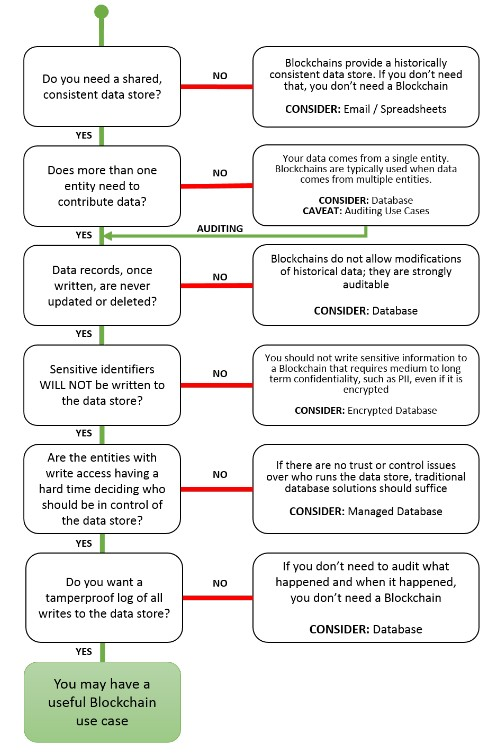
\includegraphics[width=0.7\linewidth]{Figures/Selection_107.jpg}}
    \caption{Diagrama de flujo para determinar un caso de uso Blockchain. De \cite{nist}.}
    \label{fig:use_case_diagram}
\end{figure}

Debido a las confusiones sobre la utilidad de la tecnología Blockchain en una gran cantidad de escenarios, existe una variedad de literatura que describe como determinar un caso de uso Blockchain. Entre otros, el Instituto Nacional de Estándares y Tecnología de Estados Unidos elaboró un diagrama de flujo que ayuda a descartar fácilmente ideas que son mejor implementadas en bases de datos tradicionales.

A continuación se va a analizar el caso de uso planteado con la ayuda de la figura \ref{fig:use_case_diagram} para determinar si la implementación de un sistema de validación de información académica se beneficia de utilizar tecnología Blockchain o no.

\begin{enumerate}
    \item \textbf{¿Se necesita almacenar información de forma compartida y consistente?} Sí, ya que el prototipo apunta a permitir la validación de credenciales académicas por una variedad de entidades, que pueden ser diferentes facultades, Universidades o cualquier otro organismo que necesita determinar que una nota o una historia académica sea válida.
    \item \textbf{¿Es necesario que más que una entidad aporte datos?} Planteando el caso que la UNC reemplaza actas comunes por actas digitales, todas las facultades estarían aportando información. También es posible extender el caso de uso a varias universidades: La validación de credenciales de alumnos que cambian de universidad o quieren realizar un postgrado es facilitada si una multitud de universidades agrega datos.
    \item \textbf{¿No es necesario modificar o eliminar información una vez que fue escrita?} Para el caso del prototipo planteado, la modificación o eliminación de información no es deseada. En su lugar, se desea un historial completo inmutable de lo ocurrido: al revocar un acta, por ejemplo, se mantiene el acta original junto con su acta rectificadora.
    \item \textbf{¿No se va a escribir información sensible o personal en el ledger?} A toda información se va a aplicar un \textit{hash} antes de ser agregada al Blockchain, por ende no se va a escribir nunca información en texto plano.
    \item \textbf{¿Las entidades con acceso de escritura tienen dificultades para decidir quién debe tener el control del almacén de datos?} No existe ningún proyecto para la implementación de un sistema de validación de credenciales académicas centralizado, pero la arquitectura distribuida del Blockchain implica que cada facultad (o en un futuro, Universidad) podría sumarse con pocos recursos y en el momento que sea conveniente.
    \item \textbf{¿Desea un registro inviolable de todas las escrituras en el almacén de datos?} Sí, es crucial que la información sea imposible de alterar.
\end{enumerate}

Luego del análisis efectuado, es posible concluir que el uso de Blockchain para el caso planteado tiene mayores beneficios sobre una base de datos tradicional.

\section{Funcionalidades} \label{sec:funcionalidades}

Luego de la entrevista y de la evaluación del caso de uso, se consideran necesarias las siguientes funcionalidades para el prototipo:

\begin{itemize}
    \item El prototipo debe consistir de un Blockchain con un mínimo de dos organizaciones con dos \textit{peers} cada uno, que comparten información a través de un canal.
    \item Por ende, todos los \textit{peers} deben poder acceder al mismo conjunto de información y el mismo \textit{chaincode}.
    \item El prototipo debe ser capaz que recibir credenciales académicas en texto plano, aplicar una función \textit{hash} a los datos e invocar el \textit{chaincode} correspondiente para que dicha información sea agregada al Blockchain.
    \item Se debe proporcionar la funcionalidad de verificar la existencia de una cierta porción de información: Para validar una nota por ejemplo, se debe poder ingresar la información correspondiente, el prototipo debe aplicar una función \textit{hash} a ella y buscar una coincidencia en el Blockchain para confirmar la validez.
    \item Es necesario proveer la posibilidad de corregir información: Si se requiere revocar un acta, tiene que ser posible agregar su acta rectificativa. Luego el acta original debe ser considerada inválida y ya no debe ser utilizada para validaciones.
\end{itemize}

\section{Definición de los Componentes}

Con el fin de implementar las funcionalidades descritas en la sección \ref{sec:funcionalidades}, en primer lugar se definen los componentes del prototipo en su totalidad.

\begin{enumerate}
    \item \textbf{La red Blockchain: } Se requiere una red de Hyperledger Fabric, compuesta por organizaciones que representan facultades y \textit{peers} que comparten información a través de un canal. El prototipo va a simular tres facultades generando tres organizaciones, cada una con dos \textit{peers}. De esa forma existe redundancia para cada organización: si un \textit{peer} falla, el otro sigue disponible. Además, cada organización tiene que tener una Autoridad de Certificación para otorgar identidades digitales. Va a existir un solo canal al cual las tres organizaciones tienen accesos y por ende un solo \textit{ledger}.
    \item \textbf{La base de datos para el \textit{world state}: } El prototipo a implementar maneja datos a los cuales se aplicó una función de \textit{hash} antes de su almacenamiento. Utilizar el idioma de CouchDB para realizar consultas complejas sobre el estado del \textit{ledger} por ende no es posible. Por eso se eligió LevelDB como la base de datos para almacenar el \textit{world state}.
    \begin{figure}% Example image
        \center{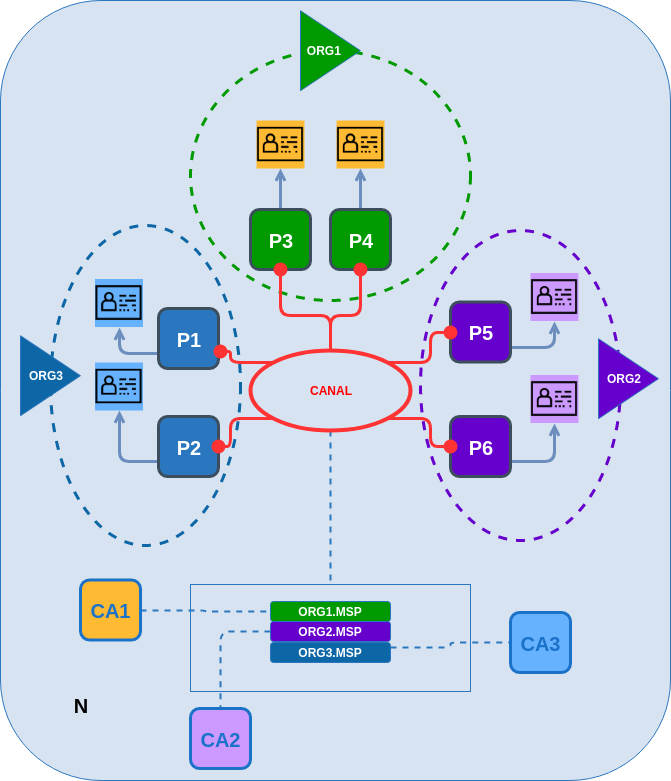
\includegraphics[width=0.8\linewidth]{Figures/network-arquitecture.png}}
        \caption{Diagrama de la red Blockchain a implementar.}
        \label{fig:bc-network}
    \end{figure}
    \item \textbf{El \textit{ordering service}: }Dada la complejidad de configurar Raft o Kafka como servicio de ordenamiento para Hyperledger Fabric se optó por Solo, el servicio de ordenamiento por defecto propuesto para test o pruebas de concepto. Si bien no es recomendado su uso en entornos de producción, cumple con todo lo requerido para el prototipo en cuestión.

    \item \textbf{Elección del lenguaje de programación para el Chaincode: }Las posibilidades para escribir \textit{chaincode} en Hyperledger Fabric son Go, Node.js o Java. Luego de varias pruebas con los 3 lenguajes, la decisión fue tomada a favor de Go: Con Node.js como Java la instanciación del \textit{chaincode} provocaba repetidos errores de tiempo de espera debido a \textit{bugs} en la implementación de Hyperledger Fabric.
    \item \textbf{Elección del SDK: }Hyperledger Fabric provee SDKs en los lenguajes Node.js, Java, Python y Go, dónde los últimos dos todavía no fueron lanzados oficialmente.\cite{hlf_sdks} Para el proyecto se utilizó el SDK en Node.js, ya que la documentación del mismo está muy completa y debido a que el código desarrollado puede ser fácilmente agregado a un \textit{framework} para aplicaciones web.
    \item \textbf{Desarrollo de una API: }El código escrito en Node.js es el código cliente que invoca al \textit{chaincode} a través de los \textit{peers}. Para que sea accesible a través de Internet es necesario el desarrollo de una API REST, que permita llamar las funciones con métodos HTML. La herramienta elegida para esa tarea es Express, un \textit{framework} minimalista y flexible para aplicaciones web y APIs. Está escrito en Javascript, de modo que la integración de las funciones escritas con el SDK se puede realizar sin inconvenientes.
    
    \begin{figure}[H] % Example image
        \center{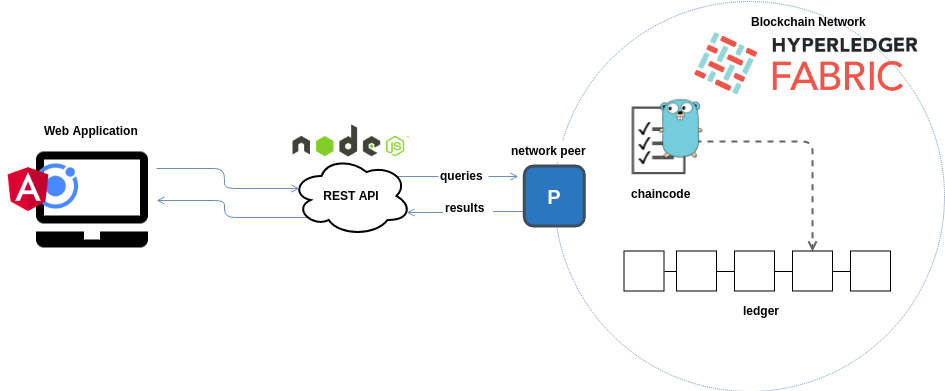
\includegraphics[width=1.0\linewidth]{Figures/arquitecture.png}}
        \caption{Diagrama general de la arquitectura junto con las tecnologías.}
        \label{fig:general_arquitecture}
    \end{figure}
    
    \item \textbf{Desarrollo de una GUI: }La API públicamente expuesta a Internet necesita un \textit{frontend}, o una interfaz web, que acceda a ella. Su funcionalidad consiste en obtener información de la API y mostrarla de forma entendible para el usuario, como también obtener datos ingresados por el usuario y enviarlos para su procesamiento a la API.
    
    Para lograr eso, se decidió utilizar Angular y Ionic: Angular es un \textit{framework} mantenido por Google para el desarrollo de \textit{Single Application Pages (SPAs)}, páginas que adaptan su contenido de forma dinámica a medida que reciben entradas del usuario, en vez de descargar páginas nuevas de un servidor. 
    
    Ionic permite agregar componentes web comúnmente usados a una aplicación escrita en Angular y agiliza así el desarrollo. A su vez viene con librerías como Apache Cordova, que permiten interactuar con dispositivos móviles. De esa forma, una misma aplicación puede ser compilada para un entorno web o un entorno móvil, dependiendo de las necesidades del desarrollador. La figura \ref{fig:ionic_stack} posiciona a Ionic en el contexto de las herramientas para el desarrollo \textit{frontend}.

    \begin{figure}[H]
        \center{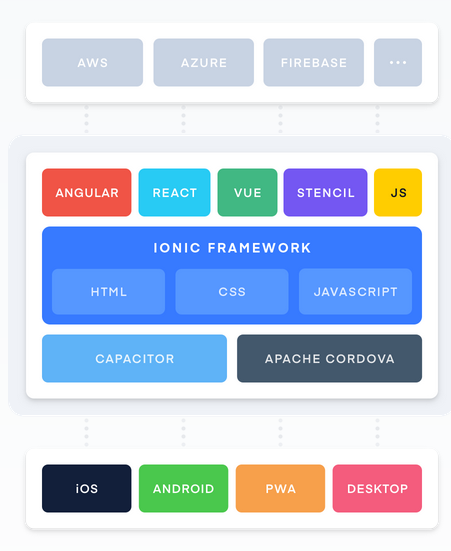
\includegraphics[width=0.6\linewidth]{Figures/Selection_182.png}}
        \caption{El rol de Ionic en el desarrollo \textit{frontend}. De \cite{what-is-ionic}.}
        \label{fig:ionic_stack}
    \end{figure}

\end{enumerate}

\section{Definición de los Requerimientos}
Para especificar el funcionamiento general del sistema, se va a hacer uso del lenguaje de modelado UML. Si bien se trata del desarrollo de un sistema distribuido con una variedad de protocolos y tecnologías, el prototipo final es un producto de \textit{software}, por lo cual un modelado en SysML no se consideró adecuado.

Para poder plantear los requerimientos, primero es necesario definir un diagrama de casos de uso, como se ve en la figura \ref{fig:use_cases}. En el diagrama se puede observar que el objetivo principal es brindar al personal administrativo un sistema de validación de información académica con las funcionalidades de agregar actas, revocarlas y validar la información contenida en las actas cargadas.

\begin{figure}[H]
    \center{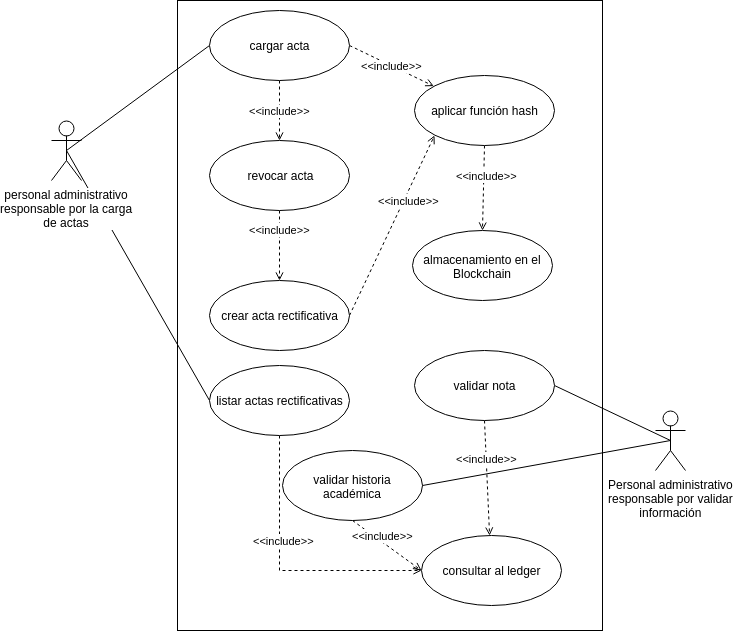
\includegraphics[width=1.0\linewidth]{Figures/use_cases.png}}
    \caption{Diagrama de casos de uso.}
    \label{fig:use_cases}
\end{figure}

Con el diagrama de caso de uso elaborado se pueden definir los siguientes requerimientos de usuario:
\begin{table}[h]
\rowcolors{2}{cyan!20}{cyan!40}
\begin{tabularx}{\textwidth}{|c|X|}
\hline
R-01 & El personal administrativo debe poder cargar la información de un acta nueva al sistema.\\
\hline
R-02 & Para poder verificar la presencia del acta cargada, debe ser posible consultar por el mismo a través de su id.\\
\hline
R-03 & En caso de que se haya cometido un error, debe ser posible revocar el acta y crear su acta rectificativa.\\
\hline
R-04 & Debe ser posible visualizar todas las actas rectificadas.\\
\hline
R-05 & Debe ser posible validar una nota con el sistema: Se debe poder ingresar la información sobre la nota con la nota en texto plano y el sistema debe avisar si la nota se encontró en el sistema o no.\\
\hline
R-06 & Debe ser posible validar la historia académica completa de un alumno de la misma forma que se puede validar una sola nota.\\
\hline
\end{tabularx}
\caption{Requerimientos de usuario.}
\label{table:req_user}
\end{table}

Luego es posible definir los requerimientos funcionales para cada uno de los componentes descritos anteriormente: la red Blockchain, la API y la interfaz gráfica. Se encuentran en los cuadros \ref{table:req_hlf} - \ref{table:req_gui}. Los requerimientos no funcionales se definieron en la tabla \ref{table:req_nofunc}.
\begin{table}[h]
\rowcolors{2}{cyan!20}{cyan!40}
\begin{tabularx}{\textwidth}{|c|X|}
\hline
RF-BC-01 & La red debe ser compuesta por 3 organizaciones y dos \textit{peers} por organización.\\
\hline
RF-BC-02 & La red debe contar con un nodo que provee el servicio de ordenamiento.\\
\hline
RF-BC-03 & Las organizaciones deben contar con una autoridad de certificación cada una para poder agregar usuarios de forma dinámica.\\
\hline
RF-BC-04 & Los \textit{peers} deben ser configurados para poder ejecutar \textit{chaincode} en el lenguaje Golang.\\
\hline
RF-BC-05 & El \textit{chaincode} debe permitir escribir un objeto JSON nuevo en el \textit{ledger}.\\
\hline
RF-BC-06 & El \textit{chaincode} debe permitir recuperar un objeto JSON teniendo la clave.\\
\hline
\end{tabularx}
\caption{Requerimientos funcionales de la red de Hyperledger Fabric.}
\label{table:req_hlf}
\end{table}

\begin{table}
    \rowcolors{2}{cyan!20}{cyan!40}
    \begin{tabularx}{\textwidth}{|c|X|}
    \hline
    RF-API-01 & La API debe proveer un método que permita la subida de un acta. Dicho método debe:
    \begin{itemize}
        \item Recibir un objeto JSON con los datos completos del acta en texto plano.
        \item Aplicar un \textit{hash} a la cabecera del acta y a cada uno de sus renglones.
        \item Formar un objeto JSON que consta del \textit{hash} de la cabecera, el nombre del usuario, un indicador de la validez del acta como el conjunto de todos los renglones del acta en formato \textit{hash}.
        \item Invocar el \textit{chaincode} mencionado en RF-BC-06 que permita escribir dicho objeto en el Blockchain.
    \end{itemize}\\
    \hline
    RF-API-02 & La API debe proveer un método que permita recuperar el acta como fue escrito en el Blockchain, haciendo uso del \textit{chaincode} descrito en el requerimiento RF-BC-06.\\
    \hline
    RF-API-03 & La API debe contar con un método que permita revocar a un acta. Para eso debe
    \begin{itemize}
        \item Verificar que el acta realmente puede ser rectificada.
        \item Marcar el acta a revocar como inválida.
        \item Generar un acta nueva con los renglones corregidos.
    \end{itemize}\\
    \hline
    RF-API-04 & La API debe proveer una función que permita indicar la validez o invalidez de una nota. Para cumplir con esa funcionalidad, debe
    \begin{itemize}
        \item Recibir el id del acta en texto plano como también la información de la nota que se encuentra en el renglón correspondiente del acta.
        \item Luego debe aplicar la función \textit{hash} al renglón y buscar el acta indicada en el Blockchain.
        \item Por último debe verificar si existe una coincidencia entre uno de los renglones recuperados y el calculado.
    \end{itemize}\\
    \hline
    RF-API-05 & La API debe poder indicar si una historia académica es válida o no, recibiendo la información necesaria y procediendo igual que en los pasos del requerimiento RF-API-04.\\
    \hline
    RF-API-06 & La API debe notificar cualquier tipo de error: En el caso que un acta no fue encontrado o en el caso de un problema de conexión o autenticación con el Blockchain.\\
    \hline
\end{tabularx}
\caption{Requerimientos funcionales de la API.}
\label{table:req_api}
\end{table}

\begin{table}[h]
    \rowcolors{2}{cyan!20}{cyan!40}
    \begin{tabularx}{\textwidth}{|c|X|}
    \hline
    RF-GUI-01 & La GUI debe contar con una página que permite la selección y ejecución de las siguientes tareas:
    \begin{enumerate}
        \item Cargar un acta nueva al sistema.
        \item Buscar un acta con su id.
        \item Validar una nota.
        \item Validar una historia académica.
        \item Revocar un acta.
        \item Consultar todos los actas rectificadas.
    \end{enumerate}\\
    \hline
    RF-GUI-02 & Para poder cumplir con cada tarea, la GUI debe proveer campos que permitan al usuario ingresar los datos necesarios para efectuar la tarea.\\
    \hline
    RF-GUI-03 & La GUI debe estar en los idiomas inglés y español. \\
    \hline
    RF-GUI-04 & Durante el tiempo de ejecución de consultas o escrituras en el Blockchain, la GUI debe indicar esto mismo al usuario.\\
    \hline
    RF-GUI-05 & La GUI debe notificar el éxito o fracaso de cada operación debidamente al usuario.\\
    \hline
    \end{tabularx}
    \caption{Requerimientos funcionales de la interfaz gráfica de usuario. (\textit{Graphical User Interface})}
    \label{table:req_gui}
\end{table}

\begin{table}[h]
    \rowcolors{2}{cyan!20}{cyan!40}
    \begin{tabularx}{\textwidth}{|c|X|}
    \hline
    RNF-01 & El sistema debe contar con pruebas y tests integrales de los seis requerimientos de usuario.\\
    \hline
    RNF-02 & El código del \textit{chaincode} debe estar escrito en el lenguaje Golang, la API debe desarrollarse en Node.js y para la Interfaz Gráfica se debe usar Typescript.\\
    \hline
    RNF-03 & La GUI debe indicar éxito o fracaso de una operación en un tiempo no mayor a los diez segundos.\\
    \hline
    RNF-04 & La GUI debe contar con un instructivo para que un usuario sin conocimiento previo puede aprender a utilizar el sistema.\\
    \hline
    \end{tabularx}
    \caption{Requerimientos no funcionales del sistema.}
    \label{table:req_nofunc}
\end{table}

Para poder comprender mejor cúal es la relación estructural entre las diferentes tecnologías empleados en el prototipo, se ofrece un diagrama de componentes, realizado en la figura \ref{fig:components}. Se distinguen 3 componentes principales: El \textit{frontend}, la aplicación y la red de Hyperledger Fabric. La aplicación se divide en el código funcional de la aplicación en sí, que convierte, por ejemplo, las actas en texto plano a un \textit{hash}, y el SDK de Hyperledger Fabric que brinda las librerías necesarias para invocar \textit{chaincode} en los diferentes \textit{peers} a través de una interfaz \textit{shim}.

\begin{figure}[H]
    \center{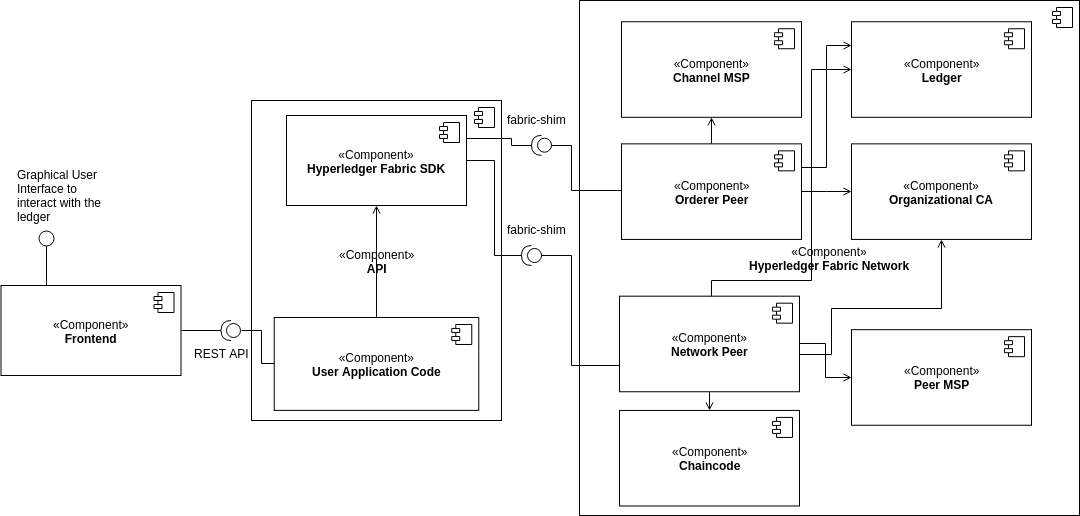
\includegraphics[width=1.0\linewidth]{Figures/components.png}}
    \caption{Diagrama de componentes.}
    \label{fig:components}
\end{figure}


\section{Definición del Comportamiento}
Para poder entender cómo interactúan los componentes diagramados, se emplearon dos diagramas de secuencia. El primero, la figura \ref{fig:secuencia1}, muestra el flujo de mensajes en el caso de una lectura del \textit{ledger}, por ejemplo para verificar la validez de un acta. En el diagrama se puede observar lo que ya se describió en la sección \ref{sec:aplicaciones_y_redBC}: Para realizar una lectura, es necesario interactuar con un solo \textit{peer} de la red. Éste puede ejecutar el \textit{chaincode} sobre su copia del \textit{ledger} local y proveer resultados sin tener que involucrar otros participantes.

\begin{figure}
    \center{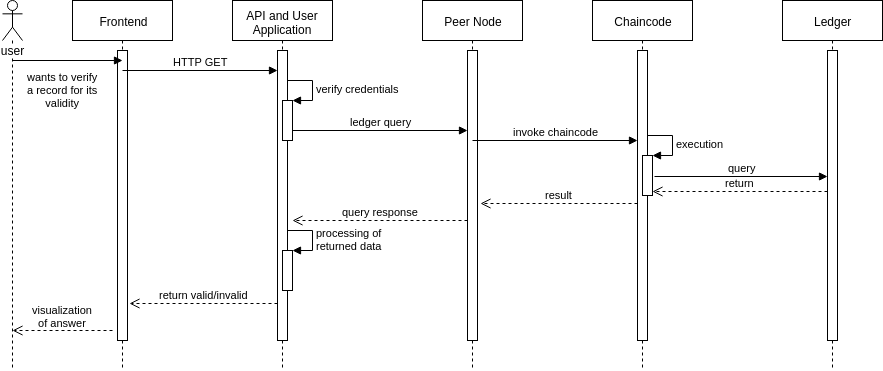
\includegraphics[width=1.0\linewidth]{Figures/sequence1.png}}
    \caption{Diagrama de secuencia para lecturas del \textit{ledger}.}
    \label{fig:secuencia1}
\end{figure}

En la figura \ref{fig:secuencia2} se puede observar el diagrama de secuencia para caso de escritura del \textit{leger}: La aplicación envía una propuesta de aprobación de la transacción (\textit{endorsement proposal}) a una cantidad definida de \textit{peers}. En el diagrama se ve que la propuesta se envía a tres \textit{peers}, pero pueden ser más o menos según la política de aprobación establecida por las organizaciones. Cada \textit{peer} ejecuta el \textit{chaincode} correspondiente y retorna los resultados a la aplicación, cuya obligación es verificar que coinciden. Luego, esta envía un mensaje con todas las respuestas al servicio que ordena las transacciones. Cuando un bloque nuevo es creado, las transacciones en cuestión van a estar incluidas en él y todos los \textit{peers} controlan que se encuentran válidas y que se respetaron las políticas de aprobación. Una vez que terminaron, un \textit{peer} notifica la aplicación para que el usuario pueda saber si la escritura en el Blockchain fue exitosa o no.

\begin{figure}[H]
    \center{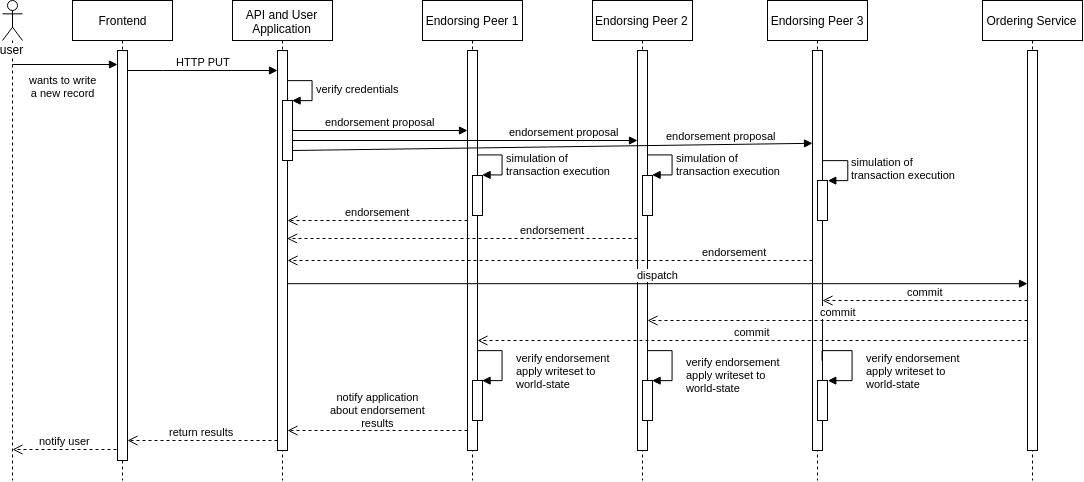
\includegraphics[width=1.0\linewidth]{Figures/sequence-write.png}}
    \caption{Diagrama de secuencia para escrituras del \textit{ledger}.}
    \label{fig:secuencia2}
\end{figure}

\section{Riesgos}
La evaluación de riesgos de un proyecto busca posibles eventos no deseados que pueden perjudicar o amenazar al proyecto con el objetivo de minimizarlos o, en el caso de que ocurran, controlar su impacto sobre el proyecto.

El objetivo de la presente sección es establecer criterios, identificar posibles riesgos, asignar prioridades a los mismos, evaluar su probabilidad y encontrar estrategias que permiten resolver los mismos o minimizar sus efectos.

\subsection{Criterios}
Los riesgos se clasifican según dos criterios: su probabilidad y la gravedad en el caso de su ocurrencia. A continuación figuran las siguientes probabilidades y gravedades que se tuvieron en cuenta según \cite{sommerville}:

\begin{enumerate}
    \item Riesgo muy bajo (\textless10\%)
    \item Riesgo bajo (10 - 25\%)
    \item Riesgo moderado (25 - 50\%)
    \item Riesgo alto (50 - 75\%)
    \item Riesgo muy alto (\textgreater75\%)
\end{enumerate}

\begin{enumerate}
    \item Efectos insignificantes
    \item Efectos tolerables
    \item Efectos graves
    \item Efectos catastróficos
\end{enumerate}

La combinación de ambos criterios permite priorizar los riesgos teniendo en cuenta ambos factores.
\begin{table}[h]
    \begin{tabular}{|c|c|c|c|c|}
    \hline
    \textbf{Probabilidad/Efecto}& \textbf{Insignificante} & \textbf{Tolerable} & \textbf{Grave} & \textbf{Catastrófico}\\
    \hline
    \textbf{Muy baja} &\cellcolor{YellowGreen} &\cellcolor{YellowGreen} &\cellcolor{YellowGreen} & \cellcolor{yellow}\\
    \hline
    \textbf{Baja} & \cellcolor{YellowGreen} & \cellcolor{YellowGreen} & \cellcolor{yellow} & \cellcolor{yellow}\\
    \hline
    \textbf{Moderada} & \cellcolor{YellowGreen} & \cellcolor{yellow} &\cellcolor{yellow} & \cellcolor{red}\\
    \hline
    \textbf{Alta} & \cellcolor{yellow} & \cellcolor{yellow} & \cellcolor{red} & \cellcolor{red} \\
    \hline
    \textbf{Muy alta} &\cellcolor{yellow} & \cellcolor{red}& \cellcolor{red}&\cellcolor{red}\\
    \hline
    \end{tabular}
    \caption{Probabilidad de riesgos vs. su efecto}
\end{table}
En base a la combinación realizada, se consideran los riesgos que se encuentran dentro del área verde como riesgos de menor prioridad, los riesgos en el área amarilla como riesgos de prioridad intermedia y los riesgos en el área roja como riesgos de prioridad alta.
\subsection{Identificación de Riesgos}
En la primera etapa de la gestión de riesgos, se buscan los posibles riesgos relacionados al proyecto, distinguiendo las 5 categorías siguientes:
\begin{itemize}
    \item \textbf{Riesgos de tecnología:} Riesgos relacionados a hardware o \textit{software} con el que se está desarrollando el proyecto.
    \item \textbf{Riesgos personales:} Relacionados con el personal en el equipo de desarrollo.
    \item \textbf{Riesgos de requerimientos:} Surgen de modificaciones de los requerimientos.
    \item \textbf{Riesgos de estimación:} relacionados a la estimación de recursos requeridos para el desarrollo del proyecto.
\end{itemize}
Los riesgos que se identificaron para el presente proyecto integrador figuran en la tabla \ref{identification_risks}.
\begin{table}[h]
    \begin{tabular}{|m{2cm}|m{7.5cm}|m{3.5cm}|}
    \hline
    \textbf{Código} & \textbf{Descripción} & \textbf{Tipo de riesgo}\\
    \hline
    Riesgo-01 & Problemas de funcionamiento o avería de la PC de desarrollo durante el tiempo de desenvolvimiento. & Tecnológico\\
    \hline
    Riesgo-02 & Incompatibilidad de versiones o librerías instaladas en la máquina de desarrollo con los \textit{frameworks} usados. & Tecnológico \\
    \hline
    Riesgo-03 & Funcionalidades sin implementar en el \textit{framework} de Hyperledger Fabric. & Requerimientos\\
    \hline
    Riesgo-04 & Demoras durante el desarrollo del proyecto debido a trabajo u otros inconvenientes personales. & Personales y Estimación \\
    \hline
    Riesgo-05 & Abandono del proyecto. & Personal \\
    \hline
    Riesgo-06 & Errores en la implementación de los \textit{frameworks} elegidos. & Tecnológico, Requerimientos y Estimación\\
    \hline
    Riesgo-07 & Falta de conocimiento para el uso de los \textit{frameworks}, del \textit{software} o los lenguajes de programación elegidos. & Estimación \\
    \hline
    Riesgo-08 & Falta de documentación o soporte de los \textit{frameworks} elegidos. & Estimación \\
    \hline
    Riesgo-09 & Rechazo de la implementación por parte del usuario, debido a desconfianza que genera una nueva tecnología. & Estimación \\
    \hline 
    \end{tabular}
    \caption{Riesgos identificados para el proyecto}
\label{identification_risks}
\end{table}

\subsection{Análisis de Riesgos}
\newcolumntype{C}[1]{>{\centering\arraybackslash}m{#1}}
En el cuadro \ref{analisys_risks} se ordenaron los riesgos según su importancia luego de estimar probabilidad e indicar el efecto.
\begin{table}
    \begin{tabular}{|C{2cm}|m{3.5cm}|C{2.4cm}|C{2.5cm}|C{2.4cm}|}
    \hline
    \textbf{Código} & \textbf{Riesgo} & \textbf{Probabilidad} & \textbf{Efecto} & \textbf{Importancia}\\
    \hline
    Riesgo-02 & Incompatibilidad de versiones o librerías instaladas en la máquina de desarrollo con los \textit{frameworks} usados. & Moderada & Insignificante &\cellcolor{YellowGreen} Prioridad baja\\
    \hline
    Riesgo-01 & Problemas de funcionamiento o avería de la PC de desarrollo durante el tiempo de desenvolvimiento. & Baja & Grave & \cellcolor{yellow} Prioridad Intermedia\\
    \hline
    Riesgo-03 & Funcionalidades sin implementar en el \textit{framework} de Hyperledger Fabric. & Alta & Tolerable & \cellcolor{yellow}Prioridad Intermedia\\
    \hline
    Riesgo-05 & Abandono del proyecto. & Muy baja & Catastrófico & \cellcolor{yellow}Prioridad Intermedia\\
    \hline
    Riesgo-06 & Errores en la implementación de los \textit{frameworks} elegidos. & Alta & Tolerable & \cellcolor{yellow} Prioridad intermedia\\
    \hline
    Riesgo-07 & Falta de conocimiento para el uso de los \textit{frameworks}, del \textit{software} o los lenguajes de programación elegidos. & Alta & Tolerable &\cellcolor{yellow} Prioridad intermedia\\
    \hline
    Riesgo-08 & Falta de documentación o soporte de los \textit{frameworks} elegidos. & Moderada & Grave &\cellcolor{yellow} Prioridad intermedia \\
    \hline   
    Riesgo-04 & Demoras durante el desarrollo del proyecto debido a trabajo u otros inconvenientes personales. & Alta & Grave & \cellcolor{red}Prioridad alta\\
    \hline
    Riesgo-09 & Rechazo de la implementación por parte del usuario, debido a desconfianza que genera una nueva tecnología. & Alta & Grave & \cellcolor{red}Prioridad alta\\
    \hline
    \end{tabular}
    \caption{Riesgos clasificados según su probabilidad y efecto.}
\label{analisys_risks}
\end{table}
\subsection{Planificación de Riesgos}
En la presente sección se describen las estrategias para manejar cada riesgo identificado. Los cuadros \ref{risk-strategy1} y \ref{risk-strategy2} detallan los pasos a seguir en el caso de la ocurrencia de cualquier riesgo.
\begin{table}[h]
    \begin{tabular}{|C{2cm}|m{3.5cm}|C{8cm}|}
    \hline
    \textbf{Código} & \textbf{Riesgo} & \textbf{Estrategias de Manejo del riesgo}\\
    \hline
    Riesgo-01 & Problemas de funcionamiento o avería de la PC de desarrollo durante el tiempo de desenvolvimiento. & \begin{itemize}
        \item Implementación de una estrategia de respaldo de información en la nube con repositorios de Gitlab.
        \item Realización de la operación \textit{push} al repositorio una o más veces por día.
        \item Arreglo o reemplazo de la máquina de desarrollo en el caso de una avería.
    \end{itemize}\\
    \hline
    Riesgo-02 & Incompatibilidad de versiones o librerías instaladas en la máquina de desarrollo con los \textit{frameworks}  usados. & \begin{itemize}
        \item Lectura cuidadosa de tutoriales de instalación y prerequisitos.
        \item Uso de Docker para ganar mayor flexibilidad con versiones de librerías o lenguajes de programación.
    \end{itemize}\\
    \hline
    Riesgo-03 & Funcionalidades sin implementar en el framework de Hyperledger Fabric. & Adaptación de los requerimientos a las posibilidades del \textit{framework}.\\
    \hline
    Riesgo-04 & Demoras durante el desarrollo del proyecto debido a trabajo u otros inconvenientes personales. & \begin{itemize}
        \item Comunicación fluida con director y codirector del trabajo.
        \item Reducción de obligaciones laborales y extracurriculares a lo mínimo e indispensable.
    \end{itemize}\\
    \hline
    Riesgo-05 & Abandono del proyecto &
    \begin{itemize}
        \item Comunicación fluida con director y codirector del trabajo.
        \item Definición clara del alcance del proyecto para minimizar las posibilidades de desborde en términos de tiempo y trabajo.
    \end{itemize}\\
    \hline
\end{tabular}
\caption{Estrategias de manejo de riesgos parte uno}
\label{risk-strategy1}
\end{table}

\begin{table}[h]
    \begin{tabular}{|C{2cm}|m{3.5cm}|C{8cm}|}
    \hline
    Riesgo-06 & Errores en la implementación de los \textit{frameworks} elegidos. &
    \begin{itemize}
        \item Implementación de \textit{workarounds} descritos en la documentación o páginas de seguimientos de \textit{issues} como Jira.
        \item Modificación de la implementación para poder cumplir con el requerimiento.
        \item Adaptación del requerimiento.
    \end{itemize}\\
    \hline
    Riesgo-07 & Falta de conocimiento para el uso de los \textit{frameworks}, del \textit{software} o los lenguajes de programación elegidos. & \begin{itemize}
        \item Lectura de tutoriales y realización de cursos de tiempo corto para lograr una introducción en temas cuyo desconocimiento impide el avance del proyecto.
        \item Empleo y modificación de ejemplos previstos para el aprendizaje.
        \item Consultas a programadores experimentados en los campos en cuestión.
     \end{itemize}\\
     \hline
     Riesgo-08 & Falta de documentación o soporte de los \textit{frameworks} elegidos. & \begin{itemize}
        \item Búsqueda de explicaciones adicionales en foros de usuarios como Stackoverflow.
        \item Consultas en canales de chat de desarrolladores como Slack o Rocketchat.
        \item Modificación de la implementación para poder cumplir con el requerimiento.
        \item Adaptación del requerimiento.
     \end{itemize}\\
     \hline
     Riesgo-09 & Rechazo de la implementación por parte del usuario, debido a desconfianza que genera una nueva tecnología. & \begin{itemize}
        \item Explicación de la tecnología y capacitación del personal.
        \item Prueba de piloto para identificar mejoras en cuanto a la usabilidad.
     \end{itemize}\\
     \hline
    \end{tabular}
    \caption{Estrategias de manejo de riesgos parte dos}
    \label{risk-strategy2}
\end{table}

\section{Control de Versiones}
Para el control de versiones, se utilizó un repositorio de Gitlab disponible bajo la URL \url{https://gitlab.com/ELeonhardt/final-project-codebase}

Si bien Git es una herramienta para para mejorar la colaboración entre varios programadores, también se justifica su uso cuando una sola persona está desarrollando el proyecto. Usar un repositorio permite tener acceso remoto al proyecto desde cualquier equipo, teniendo así una copia de seguridad del proyecto completo en la nube. A su vez, se mantiene un historial de versiones y en caso de ser necesario, es posible volver a una versión anterior o comparar las diferencias entre dos versiones distintas.

\newpage
 
% \chapter{Implementación} % Main chapter title
\label{Chapter5}
\lhead{Capítulo 5. \emph{Implementación}}
\setstretch{1.1} % Line spacing of 1.1
El presente capítulo describe los detalles de la implementación de los requerimientos explicados en el capítulo \ref{Chapter4}. %En la primera parte
Se desarrollará el sistema completo localmente en una computadora de uso común. Para explicar el tratamiento que recibe un acta en la aplicación, se usan diagramas de actividad detalladas y se realizan pruebas sobre cada etapa antes de proceder con la siguiente.

%En la segunda parte se describen las modificaciones necesarias para que dicho sistema pueda ser desplegado en un clúster de Kubernetes junto con las pruebas correspondientes en el ambiente de desarrollo microk8s.
\section{Implementación Local}
La implementación local del proyecto fue realizada en una Notebook MSI PL62 7RC, el sistema operativo empleado fue Ubuntu 16.04 LTS. Las características de la máquina se detallan en la figura \ref{fig:msi_c5}
\begin{figure}
    \center{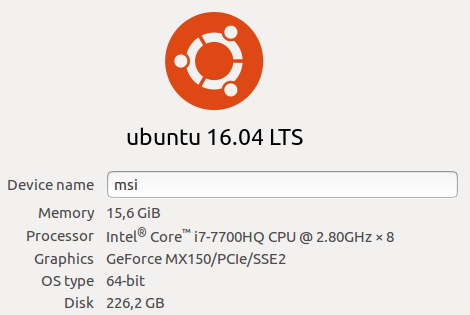
\includegraphics[width=0.6\linewidth]{Figures/Selection_189.png}}
    \caption{Características técnicas de la computadora de desarrollo.}
    \label{fig:msi_c5}
\end{figure}
\subsection{Configuración de Hyperledger Fabric}
Antes de iniciar la implementación de la aplicación en sí, es necesario configurar una red y un Blockchain con Hyperledger Fabric. Esta sección describe los pasos necesarios para cumplir con dicho objetivo.
\begin{enumerate}
    \item \textbf{Generación de certificados con la herramienta cryptogen:} Como descrito en la sección \ref{sec:identidad_de_peers}, cada integrante de la red establece su identidad a través de un certificado X.509. Hyperledger Fabric provee una herramienta llamada cryptogen que genera un conjunto de certificados y claves, así una red puede ser iniciada fácilmente con todo el material criptográfico necesario.
    
    Cryptogen lee la arquitectura deseada de la red desde un archivo con formato \textit{yaml} y genera los certificados acorde a dicho archivo. Por ende, el primer paso para la configuración de la red fue expresar su topología deseada de la siguiente forma:
    \inputminted[linenos, bgcolor=mygray]{yaml}{Listings/crypto-config.yaml}
    Las primeras cinco líneas definen una organización para el servicio que ordena las transacciones, con su nombre y dominio. Se eligió pi.elisabeth.com, donde pi es la abreviación de proyecto integrador. El dominio del cualquier \textit{peer} está compuesto por su \textit{hostname} y el dominio de la organización, por lo cual se accede como orderer.pi.elisabeth.com. Como se va a emplear el servicio \textit{solo}, se emplea a un solo host para dicha tarea.

    En la segunda sección, línea 7 a 30, se definen las organizaciones de los \textit{peers}. Para eso, se eligieron 3 facultades de la UNC y se definieron 2 \textit{peers} por cada facultad, indicados por las líneas 12, 20 y 28. La propiedad \textit{Users} está pensada para definir de forma anticipada la cantidad de usuarios que van a utilizar el Blockchain. En el caso del prototipo a desarrollar, este aspecto se va a definir de forma dinámica, por lo cual el archivo indica 1 usuario de modo que se cree solo un usuario administrador.
    
    Una vez que se pudo establecer una organización lógica de las organizaciones y \textit{peers}, es necesario generar el material criptográfico correspondiente. Para eso, se ejecuta la herramienta cryptogen en la \textit{shell} con el siguiente comando: 
    \begin{minted}{bash}
    $ ./cryptogen generate --config=./crypto-config.yaml
    \end{minted}
    Durante la ejecución se crea una carpeta en el mismo directorio que lleva el nombre \textit{crypto-config}. Dicha carpeta contiene las identidades digitales de todos los participantes de la red. Una parte de su estructura y contenidos se muestra en la figura \ref{fig:crypto-config}
    \begin{figure}
        \center{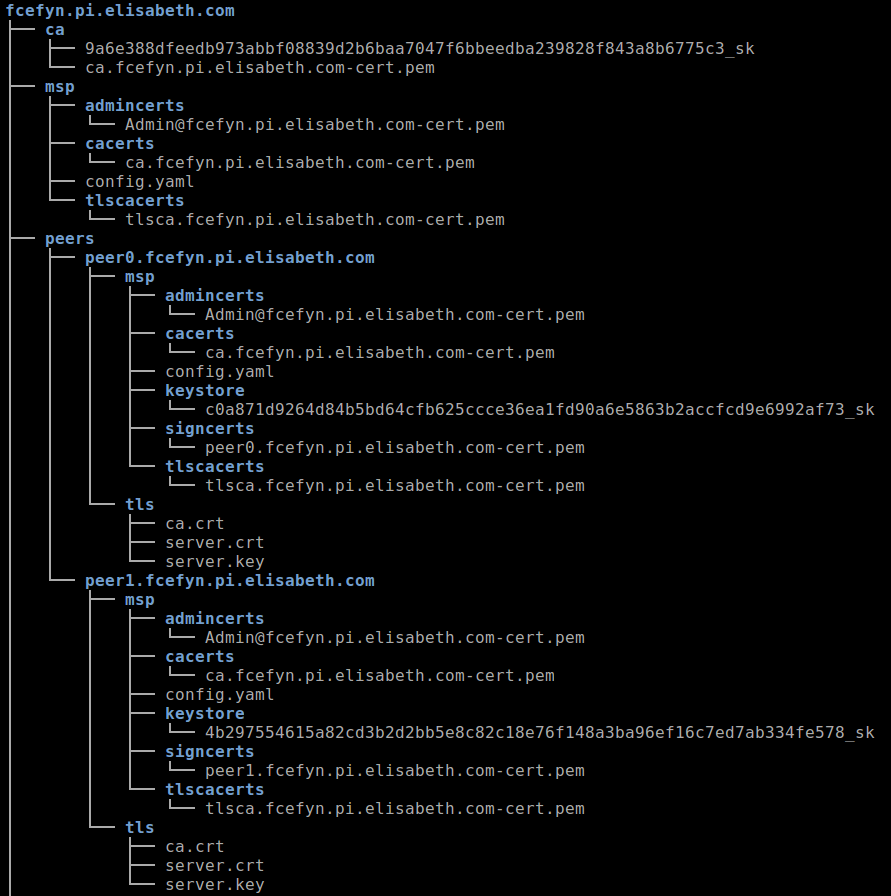
\includegraphics[width=0.8\linewidth]{Figures/Selection_191.png}}
        \caption{Directorios y archivos de la carpeta \textit{crypto-config}}
        \label{fig:crypto-config}
    \end{figure}
    \item \textbf{Generación del bloque de génesis y configuración del canal: }En el capítulo \ref{Chapter2} se explicó la arquitectura de un Blockchain: Información se almacena en bloques que contienen el \textit{hash} del bloque anterior y forman así una cadena de información. El primer bloque, llamado bloque de génesis, tiene la particularidad de almacenar solamente su propio \textit{hash}, ya que no tiene \textit{hash} de ningún bloque anterior que almacenar.
    
    En Hyperledger Fabric, el bloque de génesis cumple con un rol particular: Almacena la configuración del servicio que ordena transacciones y además información sobre las organizaciones y \textit{peers} que van a formar parte de la red. Un conjunto de organizaciones en este contexto se llama consorcio.

    Junto con el bloque de génesis se necesita la configuración del canal, que en Hyperledger Fabric describe el consorcio que va a tener acceso a un mismo \textit{ledger}.

    El bloque de génesis y la configuración del canal son llamados artefactos y son generados con la herramienta \textit{configtxgen}. Cómo \textit{cryptogen}, consume un archivo que contiene descripciones de los miembros de la red como del servicio de ordenamiento de transacciones. A continuación se van a describir las dos secciones más importantes del archivo de configuración:
    \inputminted[linenos, breaklines, bgcolor=mygray, firstline=97, lastline=105]{yaml}{Listings/configtx.yaml}
    En las líneas 97 a 105 se especifica el funcionamiento del servicio de ordenamiento de transacciones: Como tipo se eligió \textit{solo} (con las alternativas Raft y Kafka detalladas en la sección \ref{sec:ordering_service}) y se especificó un tiempo de espera de lote (\textit{BatchTimeout}) de dos segundos junto con un tamaño de lote (\textit{BatchSize}) de 512KB y un máximo de 99MB. Es decir, un bloque nuevo se genera cada dos segundos, sino se llegó antes al tamaño de lote definido.

    \inputminted[linenos, bgcolor=mygray, firstline=139, lastline=164]{yaml}{Listings/configtx.yaml}

    En las líneas 139 - 153 se define la configuración que se guarda en el bloque de génesis: Se compone por un consorcio, es decir, las tres organizaciones ya identificadas en el archivo crypto-config.yaml y la organización responsable de ordenar transacciones, aqui llamada OrdererOrg.
    
    En las líneas 154 - 163 se especifican las organizaciones que van a tener acceso al mismo canal.

    El bloque de génesis se genera con el siguiente comando:
    \begin{minted}[breaklines]{bash}
    $./configtxgen -profile OrgsOrdererGenesis -channelID sys-channel -outputBlock ./channel-artifacts/genesis.block
    \end{minted}
    Luego se crea la transacción de configuración del canal con
    \begin{minted}[breaklines]{bash}
    $./configtxgen -profile OrgsChannel -outputCreateChannelTx ./channel-artifacts/channel.tx -channelID pichannel
    \end{minted}
    Para que \textit{peers} pueden comunicarse entre organizaciones, al menos uno por organización necesita tener el estado de \textit{anchor peer}. Dicha configuración se realiza con los comandos siguientes: 
    \begin{minted}[breaklines]{bash}
    $./configtxgen -profile OrgsChannel -outputAnchorPeersUpdate ./channel-artifacts/famafMSPanchors.tx -channelID pichannel -asOrg famafMSP
    $./configtxgen -profile OrgsChannel -outputAnchorPeersUpdate ./channel-artifacts/fcefynMSPanchors.tx -channelID pichannel -asOrg fcefynMSP
    $./configtxgen -profile OrgsChannel -outputAnchorPeersUpdate ./channel-artifacts/fcqMSPanchors.tx -channelID pichannel -asOrg fcqMSP
    \end{minted}
    Se puede comprobar que en la carpeta channel-artifacts se encuentran los dos artefactos generados.
    \begin{figure}[H]
        \center{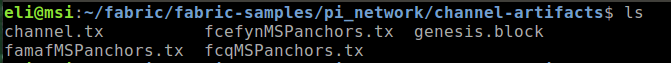
\includegraphics[width=1.0\linewidth]{Figures/Selection_199.png}}
        \caption{Artefactos generados por \textit{configtxgen}}
        \label{fig:configtxgen}
    \end{figure}

    \item \textbf{Iniciar los integrantes de la red con docker-compose: } Luego de la creación de los artefactos, el siguiente paso es iniciar todos los participantes de la red y compartirles los archivos generados. De esa forma pueden conocer su identidad y empezar a comunicarse con los demás participantes de la red. Para simular la cantidad de hosts requerida, se utilizaron las herramientas Docker y Docker Compose.
    
    La configuración de los \textit{peers}, autoridades de certificación y nodos de ordenamiento de transacciones se realizó en 3 archivos de docker-compose diferentes. El primero tiene el nombre \textit{peer-base.yaml} y define un \textit{peer} genérico con variables de entorno que aplican a todos los \textit{peers}, independiente de su organización. El segundo archivo, \textit{docker-compose-base.yaml}, describe todos los \textit{peers} que van a formar parte de la red con sus variables de entorno específicas. Un ejemplo provee la declaración del primer \textit{peer} de fcefyn:
    \inputminted[linenos, breakanywhere=true, breaklines, bgcolor=mygray, firstline=75, lastline=96]{yaml}{Listings/docker-compose-base.yaml}
    Líneas 78 y 79 muestran que el servicio extiende las propiedades descritas en \textit{peer-base.yaml}. En la sección \textit{environment} se declaran variables de entorno específicos del \textit{peer0} de la organización fcefyn y en la sección volúmenes se montan en primer lugar la transacción de configuración del canal y luego el material criptográfico generado con crypto-config.

    El tercer archivo, con el nombre \textit{docker-compose.yaml}, declara la topología completa de la red, extendiendo a \textit{docker-compose-base.yaml}. En una red llamada pi, se definen 3 autoridades de certificación, (una por organización), un total de 6 \textit{peers}, un \textit{orderer} y un contenedor auxiliar con el nombre cli.

    Para iniciar todos los contenedores, es necesario ejecutar el siguiente comando:
    \mint{bash}|$ docker-compose up -d|
    y luego se pueden ver los contenedores iniciados con el comando \mint{bash}|$ docker ps|
    \begin{figure}[H]
        \center{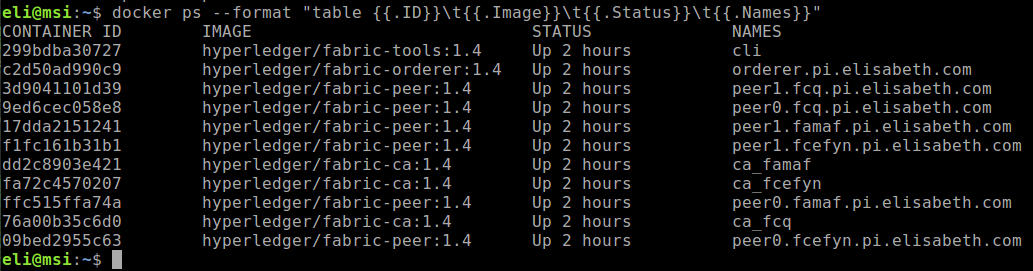
\includegraphics[width=1.0\linewidth]{Figures/Selection_193.png}}
        \caption{La red de Hyperledger Fabric desplegada con contenedores Docker}
        \label{fig:blockchain_network}
    \end{figure}
    En la figura \ref{fig:blockchain_network} se puede ver una captura en la cual figuran los contenedores previamente declarados. Se aplicó un filtro al comando para mejorar la visibilidad del resultado.
\item \textbf{Creación del canal y configuración de los peers: }Una vez que todos los contenedores se encuentran iniciados, es necesario crear el canal e indicar a todos los \textit{peers} que se unan al mismo. Para completar dicha tarea, existe el contenedor con el nombre cli, que permite ejecutar comandos en los \textit{peers} a través de una API.

Primero, se accede a la \textit{shell} del contenedor:
\begin{minted}{bash}
$ docker exec -it cli bash
\end{minted}
Luego, se ejecuta el siguiente comando para la creación del canal, haciendo uso del artefacto \textit{channel.tx} generado en el paso 2:
\begin{minted}[breaklines]{bash}
$ peer channel create -o orderer.pi.elisabeth.com:7050 -c pichannel -f ./channel-artifacts/channel.tx
\end{minted}
Para unir los demás \textit{peers} al canal, se ejecuta
\begin{minted}[breaklines]{bash}
$ peer channel join -b pichannel.block
\end{minted}
en cada \textit{peer}.

Con el fin de asegurar que el \textit{ledger} y el canal se crearon de forma exitosa, se puede inspeccionar el log de cualquier \textit{peer}:
\begin{figure}[H]
    \center{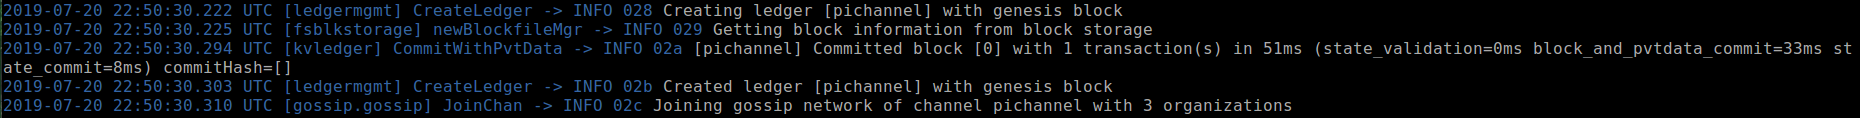
\includegraphics[width=1.0\linewidth]{Figures/Selection_197.png}}
    \caption{Mensajes del log de un \textit{peer} indicando que \textit{ledger} y canal se crearon de forma exitosa.}
    \label{fig:succesful_ledger}
\end{figure}

Por último, se aplican los artefactos que precisan los \textit{anchor \textit{peers}}. Aquí se ve el comando para la definición del \textit{anchor peer} de la organización fcq:
\begin{minted}[breaklines]{bash}
$ peer channel update -o orderer.pi.elisabeth.com:7050 -c pichannel -f ./channel-artifacts/fcqMSPanchors.tx
\end{minted}
En la figura \ref{fig:all_peers} se puede ver que todos los \textit{peers} se unieron al canal y que el peer0 de la organización fcq tiene conocimiento de todos los demás \textit{peers} de la red.
\begin{figure}[H]
    \center{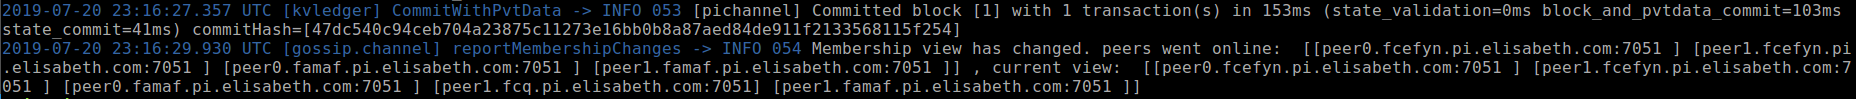
\includegraphics[width=1.0\linewidth]{Figures/Selection_198.png}}
    \caption{Mensajes del log de peer0.fcq.pi.elisabeth.com indicando todos los \textit{peers} conocidos.}
    \label{fig:all_peers}
\end{figure}
\item \textbf{Instalación y Uso del Chaincode: }Ya se logró configurar la red con todos sus participantes, pero todavía no es posible almacenar la información en el \textit{ledger}. Antes es necesario escribir e instalar el \textit{chaincode}.

El \textit{chaincode} en Hyperledger Fabric es el equivalente de los \textit{smart contracts} en otras implementaciones, como por ejemplo Ethereum. En el contexto de este proyecto, se escribieron tres chaincodes: \textit{addRegister} para agregar un acta al \textit{ledger}, \textit{queryRegister} para consultar por un acta y \textit{queryAllRectified} para obtener todas las actas rectificadas.

El \textit{chaincode} invoca la API presente en los \textit{peers}. A continuación se puede ver la función \textit{addRegister}: 
\begin{minted}[breaklines]{go}
    func (s *SmartContract) addRegister(APIstub shim.ChaincodeStubInterface, args []string) sc.Response {

	var buffer bytes.Buffer
	APIstub.PutState(args[0], []byte(args[1]))
	return shim.Success(buffer.Bytes())
}
\end{minted}

Luego de su redacción, es necesario instalar el \textit{chaincode} en todos los \textit{peers} que lo van a utilizar. Como en el caso de la configuración del canal, eso también se hace a través del contenedor cli. El comando para la instalación es el siguiente:
\begin{minted}[breaklines]{bash}
$ peer chaincode install -n picc -v 1.0 -p github.com/chaincode/
\end{minted}
Los mensajes correspondientes en los \textit{logs} del \textit{peer} confirman la instalación correcta, visibles en la figura \ref{fig:chaincode_logs}.
\begin{figure}[H]
    \center{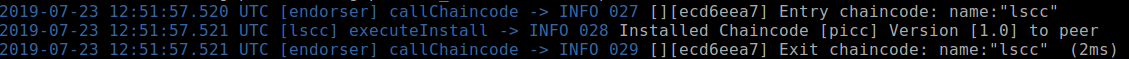
\includegraphics[width=1.0\linewidth]{Figures/Selection_203.png}}
    \caption{Mensajes del log de peer0.famaf.pi.elisabeth.com indicando la instalación correcta del \textit{chaincode}.}
    \label{fig:chaincode_logs}
\end{figure}
Luego es necesario instanciar al \textit{chaincode}, lo cual significa que se inicializa un contenedor Docker adicional en la misma red, en el cual el \textit{chaincode} se va a ejecutar. Mientras la instalación es necesaria en todos los \textit{peers}, la instanciación se requiere una sola vez.
\begin{minted}[breaklines]{bash}
$ docker exec cli peer chaincode instantiate -o orderer.pi.elisabeth.com:7050 -C pichannel -n picc -v 1.0 -c '{"Args":[]}' -P "OutOf (2, 'famafMSP.peer', 'fcefynMSP.peer', 'fcqMSP.peer')"
\end{minted}
El último argumento indica la política de aprobación: Se definió que dos \textit{peers} de diferentes organizaciones tienen que haber ejecutado el \textit{chaincode} y haber llegado al mismo resultado, caso contrario la operación no va a ser agregada al \textit{ledger}.

Por último, se verifica el funcionamiento correcto de la red invocando el \textit{chaincode} instalado. Éste tiene 3 funciones: \textit{addRegister} para agregar un acta, \textit{queryRegister} para consultar por un acta y \textit{queryAllRectified} para obtener todos los actas rectificadas.

Desde el contenedor cli, se ejecutó primero el comando siguiente:
\begin{minted}[breaklines]{bash}
$ peer chaincode invoke -o orderer.pi.elisabeth.com:7050 -C pichannel -n picc --peerAddresses peer0.famaf.pi.elisabeth.com:7051 --peerAddresses peer0.fcefyn.pi.elisabeth.com:7051 -c '{"Args":["addRegister", "UNC111", "{'UNC111':'testregister'}"]}'
\end{minted}
Para poder cumplir con la política de aprobación, la petición se envía a dos \textit{peers} de organizaciones diferentes. La información a escribir es un \textit{string} de prueba en formato JSON.
Luego se puede consultar por el acta ``UNC111'' con la función \textit{queryRegister}:
\begin{minted}[breaklines]{bash}
$ peer chaincode query -C pichannel -n picc -c '{"Args":["queryRegister","UNC111"]}'
\end{minted}
con el resultado visible en la figura \ref{fig:query_reg_call}
\begin{figure}[H]
    \center{
\includegraphics[width=1.0\linewidth]{Figures/Selection_208.png}}
    \caption{Respuesta de la llamada a la función \textit{queryRegister}}
    \label{fig:query_reg_call}
\end{figure}
\end{enumerate}
Con los pasos descritos quedan concluidas la configuración y las pruebas de la red de Hyperledger Fabric en un ambiente local.
\subsection{Automatización con un bash script}
Dada la numerosa cantidad de pasos a ejecutar, la importancia de escribir los parámetros y los variables de entorno correctamente y la necesidad de ejecutar pruebas con una red nueva, se automatizó el proceso descrito en la sección anterior mediante un \textit
{script} en el lenguaje \textit{bash}. Al ejecutarlo, 
\begin{itemize}
    \item Se eliminan todos los contenedores, volúmenes, redes y material criptográfico que pueden existir de una ejecución anterior.
    \item Se generan nuevamente los artefactos.
    \item Se inician todos los contenedores especificados en el archivo docker-compose.yaml.
    \item Se configuran canal y \textit{anchor peers}.
    \item Se instala el \textit{chaincode} en todos los \textit{peers} y se instancia.
\end{itemize}
Luego de la ejecución, es posible invocar al \textit{chaincode} directamente. El \textit{bash script} posibilita el avance rápido con los otros elementos del proyecto, ya que en caso de ocurrir errores, simplemente se genera una red con material criptográfico nuevo y sin datos previamente almacenados.

\subsection{Implementación de la Aplicación con API}
Al desarrollar la aplicación en Javascript, se partió con las funciones definidas en el ejemplo de Hyperledger Fabric disponible en \href{https://github.com/hyperledger/fabric-samples/tree/release/fabcar}{https://github.com/hyperledger/fabric-samples/tree/release/fabcar}. Luego de descargar los archivos \textit{enrollAdmin.js}, \textit{registerUser.js}, \textit{query.js} e \textit{invoke.js} junto con el respectivo \textit{package.json}, se ejecutó el comando
\begin{minted}{bash}
$ npm install
\end{minted}
Para iniciar el ambiente e instalar todos los módulos requeridos de node.js. Con el fin de que la aplicación se reinicie automáticamente cuando ocurran cambios de código, se instaló nodemon:
\begin{minted}{bash}
$ npm install nodemon --save
\end{minted}

La aplicación necesita información sobre la topología de la red a la cual conectarse. Se define a través del archivo \textit{connection.json}, que indica canales, organizaciones, \textit{peers} y autoridades de certificación. A continuación, se ve una parte del archivo en cuestión:
\inputminted[linenos, breakanywhere=true, breaklines, bgcolor=mygray, firstline=16, lastline=40]{json}{Listings/connection.json}

Las funciones separadas que se descargaron son útiles para comprobar el funcionamiento correcto del SDK, pero no es un formato conveniente para que sean invocadas desde una aplicación web. Por ende, los pasos a seguir consisten en:
\begin{enumerate}
    \item Implementar una API con el \textit{framework} Express.
    \item Embeber las funciones descargadas para que puedan acceder al Blockchain cuando se llame la API.
    \item Desarrollar y agregar las demás funciones necesarias para cumplir con los requerimientos definidos en el capítulo \ref{Chapter4}.
\end{enumerate}

\begin{enumerate}
    \item \textbf{Implementación de una API REST con el framework Express}\newline
    Se empezó con el código de un servidor web que responde a una sola consulta:
    \inputminted[linenos, breakanywhere=true, breaklines, bgcolor=mygray]{js}{Listings/example.js}
    Luego se usó el \textit{software} Postman para comprobar el correcto funcionamiento del programa.
    \begin{figure}[H]
        \center{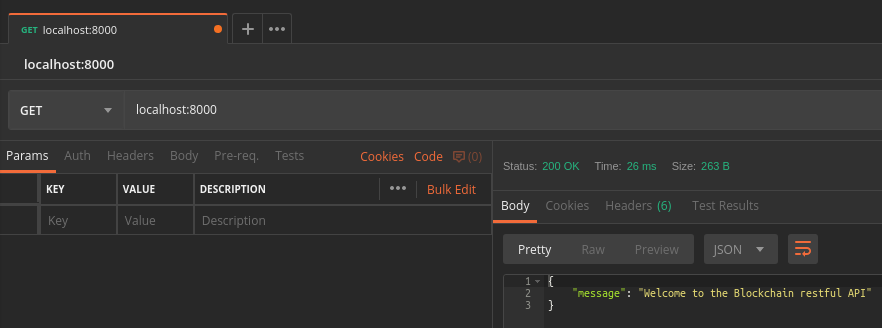
\includegraphics[width=1.0\linewidth]{Figures/Selection_213.png}}
        \caption{Prueba de la función GET con Postman}
        \label{fig:postman_first}
    \end{figure}
    En la figura \ref{fig:postman_first} se puede observar que la aplicación está funcionando correctamente, ya que devuelve el mensaje \textit{``Welcome to the Blockchain restful API''}.
    \item \textbf{Ampliación de la API para registrar usuarios}\newline
    En primer lugar, es necesario inscribir al administrador y luego registrar al usuario que va a invocar al \textit{chaincode}. En el contexto del proyecto integrador, se va a crear un solo usuario con el nombre \textit{user1} para la organización fcefyn, sin embargo es posible ampliar la cantidad de usuarios fácilmente con la ayuda de la función ya escrita.
    Como el foco de la aplicación es cargar actas y validar sus entradas, la API controla de forma automática que \textit{admin} y \textit{user1} estén registrados:
    \begin{minted}[linenos, breakanywhere=true, breaklines, bgcolor=mygray]{js}
    app.listen(3000, () => {
        console.log("Server running on port 3000");
        enroll_admin.enrollAdmin().then(
            success => {
                setTimeout(() => register_user.registerUser(), 1000)
            })
        });
    \end{minted}
\end{enumerate}
\subsubsection{Desarrollo de la función \textit{add\_register}}
La primera función a desarrollar agrega actas al Blockchain, ya que se necesitan datos presentes en el \textit{ledger} para poder programar funciones futuras que, por ejemplo, validen dichos datos.

Un acta en el contexto de este proyecto tiene formato JSON. En una cabecera se describen los atributos del acta en sí y una cantidad arbitraria de renglones especifica los datos de los alumnos. Un ejemplo con dos renglones sigue a continuación:
\begin{minted}[linenos, breakanywhere=true, breaklines, bgcolor=mygray]{json}
{
    "UNC201200017":{
    "Acta Nr":"201200017",
    "Año academico":"2016",
    "Actividad":"(1001) Análisis matemático 1a",
    "Fecha Examen":"05/10/2016",
    "Turno": "Octubre 2016",
    "Ubicación": "Sede Av Santa Fe",
    "Mesa": "A",
    "Llamado": "Llamado del Turno Octubre 2016"
    },

    "Renglones":{
        "1":{
        "Appellido y Nombre":"Acevedo Mauricio German",
        "Identificacón:":"DNI 4260181",
        "Instancia": "Regular",
        "Fecha": "05/10/2017",
        "Nota": 2,
        "Letras": "dos",
        "Resultado": "reprobado"},

        "2":{
        "Appellido y Nombre":"Alaniz Roxana Aide",
        "Identificacón:":"DNI 9609175",
        "Instancia": "Regular",
        "Fecha": "05/10/2017",
        "Nota": 8,
        "Letras": "ocho",
        "Resultado": "aprobado"}
    }
}
\end{minted}
La figura \ref{fig:actividad_add_register} muestra la lógica de la función implementada: Se aplican funciones \textit{hash} al id, a la cabecera y a cada uno de los renglones y luego se genera un JSON nuevo con dicha información que tiene el siguiente aspecto: 
\begin{minted}[linenos, breakanywhere=true, breaklines, bgcolor=mygray]{json}
{
  "id": "d7ce098a17e4bb0cc49041382beb8577",
  "header": "8bb106442e641e7af465bd40cf54375e",
  "validity": "valid",
  "creator": "user1",
  "lines": 
   { "1": "81116f6d2bdf1728e17d0258d54a74e9",
     "2": "b1af6ddd90993bdd9763e45e280cbb6b" }
}
\end{minted}
\begin{figure}
    \center{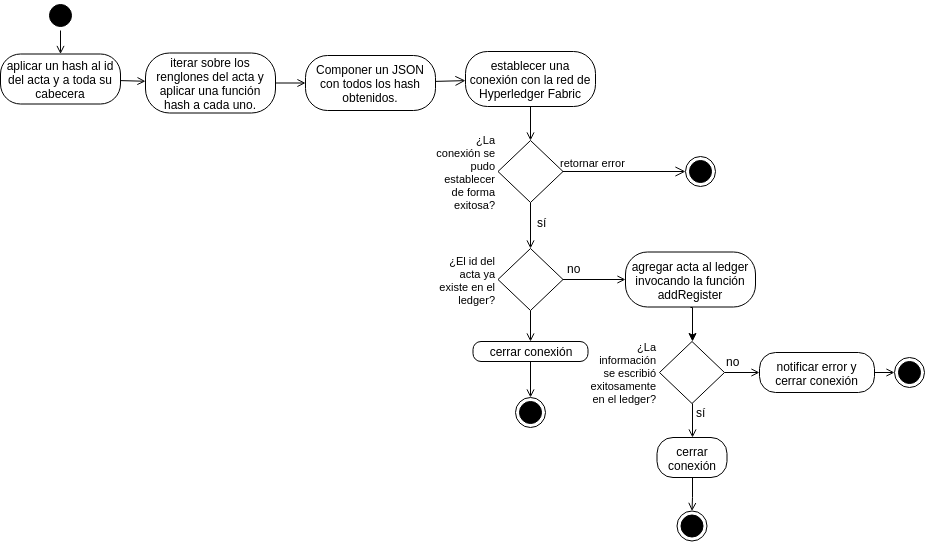
\includegraphics[width=0.8\linewidth]{Figures/actividad1.png}}
    \caption{Diagrama de actividad de la función add\_register}
    \label{fig:actividad_add_register}
\end{figure}

Luego, se establece una conexión con la red de Hyperledger Fabric y se invoca el \textit{chaincode} \textit{queryRegister} con el id del acta como parámetro. Dicha consulta se hace para verificar que el acta todavía no fue agregada al Blockchain. Si se encuentra una entrada con el mismo id, la conexión se cierra y la API devuelve un mensaje de error especificando que el acta ya existe. Caso contrario se invoca a la función \textit{addRegister} con los parámetros ``UNC201200017'' y el JSON con los \textit{hash}. Si la operación de escritura fue exitosa, la API devuelve el mensaje ``El acta se subió exitosamente'' como se ve en la figura \ref{fig:add_register_api}.

\begin{figure}[H]
    \center{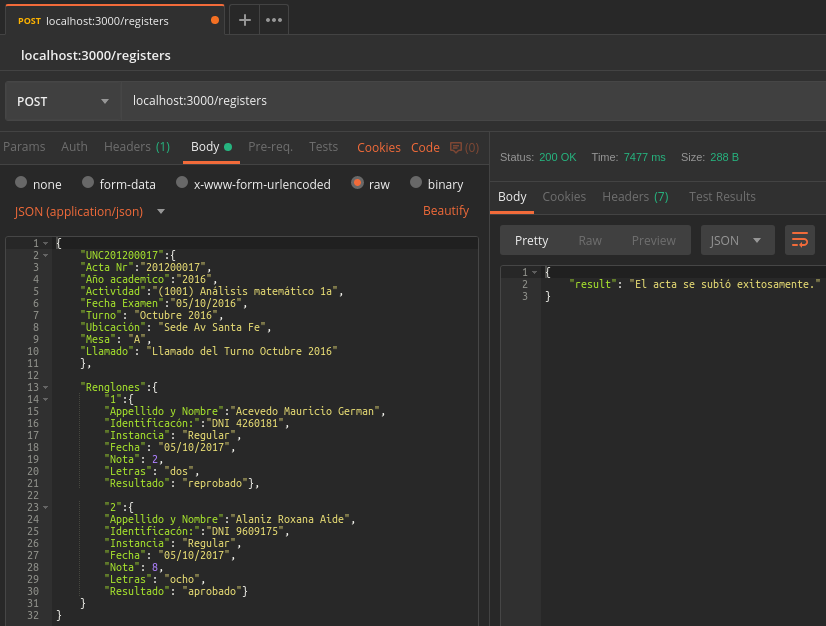
\includegraphics[width=0.7\linewidth]{Figures/Selection_220.png}}
    \caption{Subida exitosa de un acta a través de la API.}
    \label{fig:add_register_api}
\end{figure}

\subsubsection{Desarrollo de la función \textit{query}}
La función \textit{query} está pensada para poder comprobar el funcionamiento correcto del sistema, no para el uso del personal administrativo. Su objetivo es recuperar el acta como se agregó al Blockchain haciendo uso del \textit{chaincode} \textit{queryRegister}.
En la figura \ref{fig:query_register_api} es posible ver la llamada al Blockchain junto a su respuesta constando de la información previamente subida.
\begin{figure}[H]
    \center{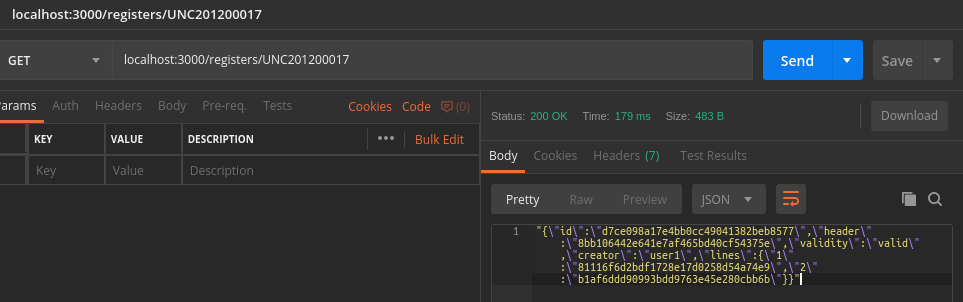
\includegraphics[width=1.0\linewidth]{Figures/Selection_221.png}}
    \caption{Consulta de un acta por Postman.}
    \label{fig:query_register_api}
\end{figure}
En el caso de consultar por un id inexistente, la API responde con el mensaje ``Acta no encontrada.''

\subsubsection{Desarrollo de la función \textit{check\_validity}}
Luego de haber subido un acta al Blockchain, ya es posible implementar la función que verifique la validez de una nota. La secuencia de pasos a implementar se puede ver en la figura  \ref{fig:validate_grade}.
\begin{figure}[H]
    \center{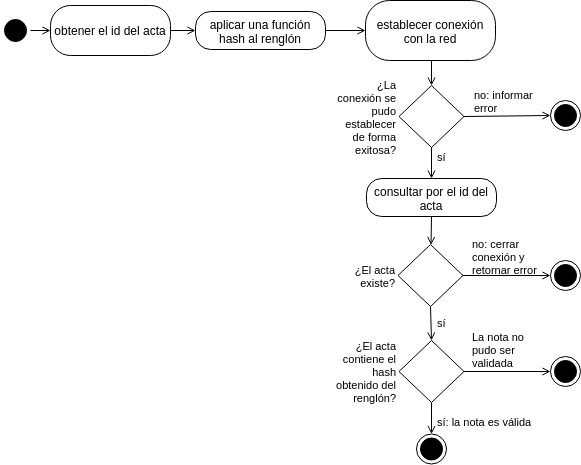
\includegraphics[width=0.6\linewidth]{Figures/actividad3.png}}
    \caption{Diagrama de actividad para el caso de validación de una nota.}
    \label{fig:validate_grade}
\end{figure}
En primer lugar, se envía un objeto JSON a la API que contiene el id del acta junto al renglón que se quiere validar. La API aplica la misma función \textit{hash} al renglón que fue aplicada en el momento de subir el acta. Luego se establece una conexión con la red y se consulta por el acta en cuestión. Si éste existe, se busca el \textit{hash} recientemente calculado entre los renglones del acta almacenada en el Blockchain. Si existe una coincidencia, la nota es válida, en caso contrario, la nota se declara inválida. En la figura \ref{fig:validate_grade_api}, se ve el caso de la validación exitosa de la nota de un alumno ficticio con el nombre Mauricio German Acevedo.
\begin{figure}[H]
    \center{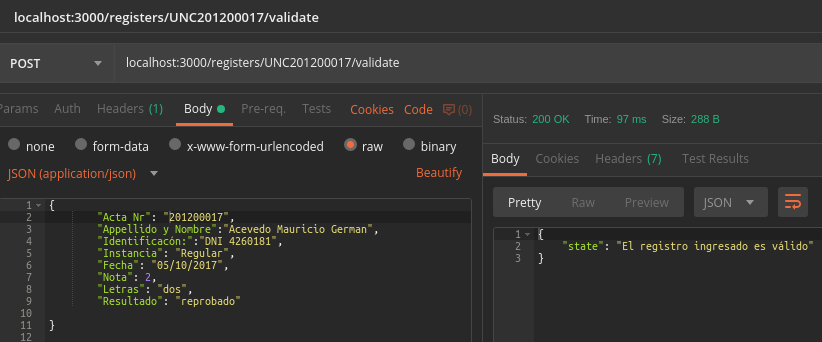
\includegraphics[width=0.8\linewidth]{Figures/Selection_222.png}}
    \caption{Validación exitosa de una nota.}
    \label{fig:validate_grade_api}
\end{figure}
\subsubsection{Desarrollo de la función \textit{verify\_history}}
La función que verifica la validez de una historia académica funciona de forma muy parecida a la que verifica la validez de una sola nota: La API itera sobre los renglones, aplica la función \textit{hash} a cada uno y busca una coincidencia con los \textit{hash} presentes en las actas obtenidos. La figura \ref{fig:validate_history_api} muestra la consulta realizada junto con el resultado que la API entrega: Como hasta el momento solo se agregó un acta al Blockchain, tres de los cuatro actas no fueron encontradas. La historia académica completa solamente puede ser considerada válida si la totalidad de respuestas indica notas válidas.
\begin{figure}
    \center{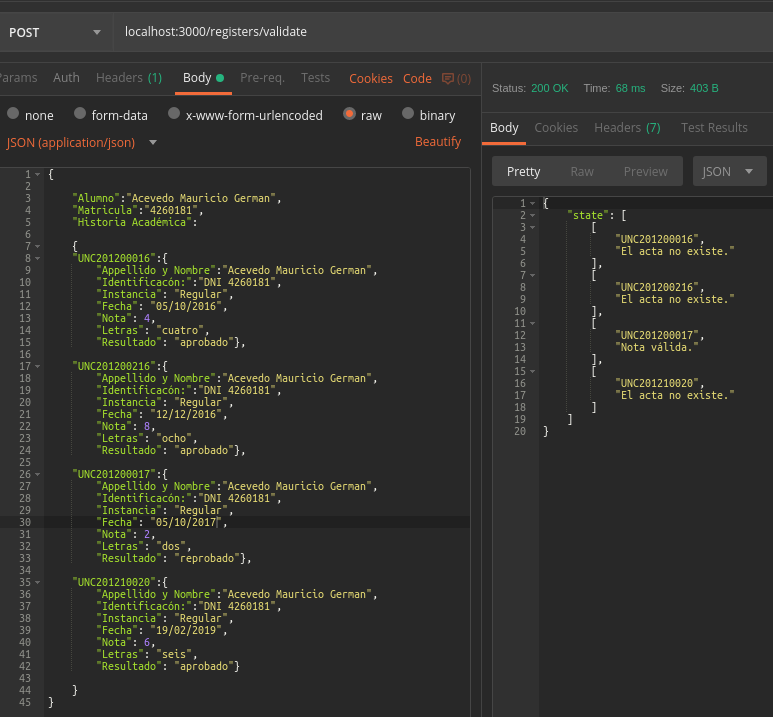
\includegraphics[width=0.9\linewidth]{Figures/Selection_223.png}}
    \caption{Validación de una historia académica.}
    \label{fig:validate_history_api}
\end{figure}
\subsubsection{Desarrollo de la función \textit{add\_revoked}}
Ahora que ya es posible subir actas y validar notas, falta la implementación del requerimiento que permite revocar un acta. El diagrama de actividad para dicha función se puede ver en la figura \ref{fig:activity_revoke}. Para demostrar el flujo con un ejemplo, se va a asumir que ocurrió un error al reprobar el alumno Mauricio German Acevedo en el acta 201200017 y que es necesario corregir la nota por un cuatro. La corrección afectaría a un solo renglón de un total de 2 renglones del acta.
Un objeto JSON muestra la información que se envía a la API para invocar las funciones correspondientes.
\begin{figure}
    \center{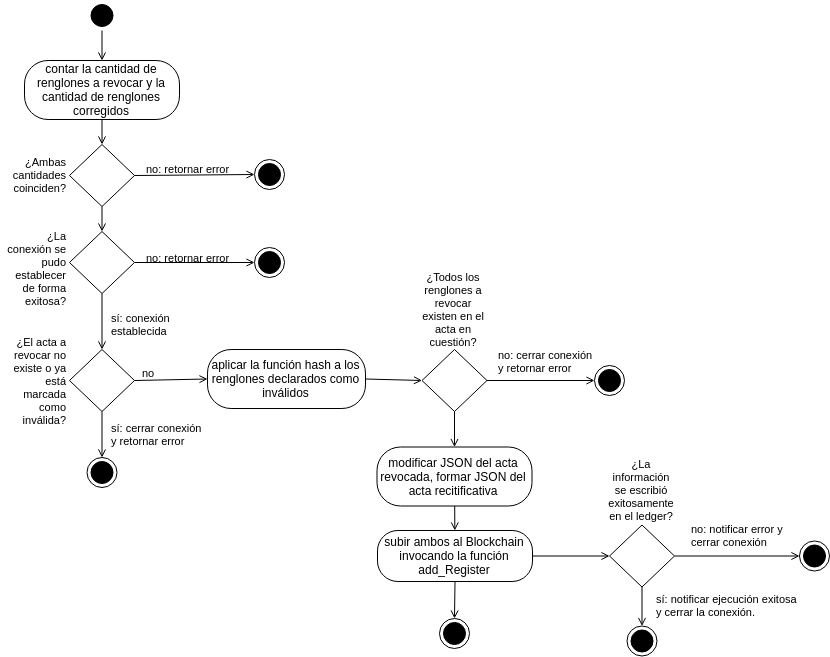
\includegraphics[width=0.7\linewidth]{Figures/actividad4.png}}
    \caption{Diagrama de actividad para revocar un acta.}
    \label{fig:activity_revoke}
\end{figure}
\begin{minted}[linenos, breakanywhere=true, breaklines, bgcolor=mygray]{json}
{    "Acta Nr":"201200017",

    "revocar":{

        "1":{
        "Appellido y Nombre":"Acevedo Mauricio German",
        "Identificacón:":"DNI 4260181",
        "Instancia": "Regular",
        "Fecha": "05/10/2017",
        "Nota": 2,
        "Letras": "dos",
        "Resultado": "reprobado"}
    },
    "corregido":{
         "1":{
        "Appellido y Nombre":"Acevedo Mauricio German",
        "Identificacón:":"DNI 4260181",
        "Instancia": "Regular",
        "Fecha": "05/10/2017",
        "Nota": 4,
        "Letras": "cuatro",
        "Resultado": "aprobado"}
	}
}
\end{minted}
Los pasos que efecúa la API son los siguientes:
\begin{enumerate}
    \item Se verifica que la cantidad de renglones a revocar coincida con la cantidad de renglones corregidos, caso contrario quedarían renglones revocados sin corregir o se corregirían renglones que no fueron revocados.
    \item Después de que la API pudo establecer una conexión con la red, verifica que el acta a revocar existe y es válida. Si no sería posible crear un acta rectificativa para un acta inexistente o una que ya tiene acta rectificativa, en cuyo caso existirían dos actas rectificativas para una sola acta revocada. En el contexto del proyecto presente, solamente es posible corregir un acta una sola vez.
    \item Si es posible revocar el acta, se aplica la función \textit{hash} a todos los renglones: los que se van a revocar y los que van a corregir los revocados. Se verifica que los renglones a revocar realmente existen en el acta en cuestión, ya que si no fuera el caso, se estaría revocando información inexistente.
    \item Si todas las verificaciones anteriores resultaran exitosas, se genera el acta nueva reemplazando los \textit{hash} de los renglones revocados por los \textit{hash} de los renglones corregidos. El id de cualquier acta rectificativa inicia con las letras RECT, para poder distinguirlo de actas que no fueron corregidas.
    
    Por otro lado, se modifica el acta revocada, cambiando el valor de la clave ``validity'' por ``invalid'' y agregando una clave ``revoked lines'' que lleva como valor los \textit{hash} de las líneas que fueron revocadas. Es necesario recordar que en el caso de una consulta al \textit{ledger} con la función \textit{query}, el \textit{peer} consulta al \textit{world state}, que siempre indica el valor más actual de un objeto almacenado. Una vez que se revocó el acta 201200017, una consulta siempre va recuperar el acta con estado inválido. Si se consulta por el historial de la misma acta, va a haber dos entradas: el original y luego el revocado.
    \item Por último, se actualiza el acta revocada y se agrega el acta rectificativa al Blockchain.
\end{enumerate}
\begin{figure}[H]
    \center{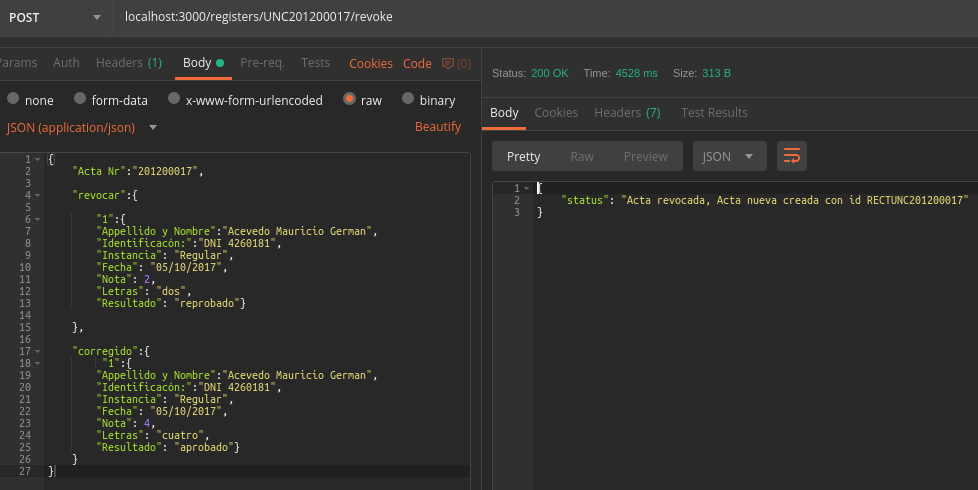
\includegraphics[width=0.9\linewidth]{Figures/Selection_224.png}}
    \caption{Creación de un acta rectificativa.}
    \label{fig:revoke_api}
\end{figure}
En la figura \ref{fig:revoke_api} se puede ver la respuesta de la API en el caso de una corrección exitosa. Se indica el id del acta rectificativa. Si ahora se hace una consulta a \textit{localhost:3000/registers/UNC201200017} (figura \ref{fig:invalid_register}), se puede ver que el estado es inválido y se agregó la clave ``revoked\_lines'', de la cual se habló anteriormente.
\begin{figure}
    \center{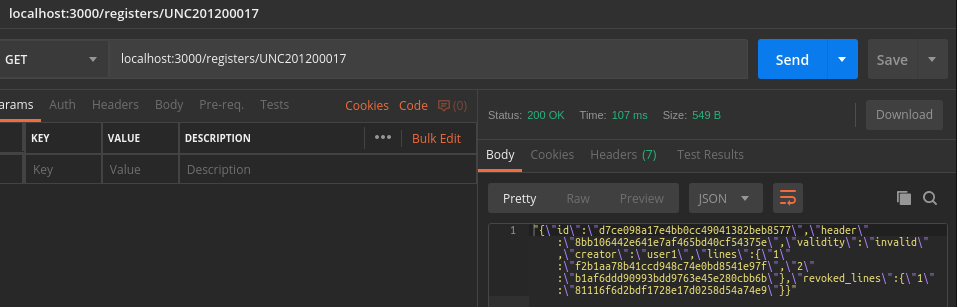
\includegraphics[width=0.9\linewidth]{Figures/Selection_225.png}}
    \caption{Consulta de un acta inválida.}
    \label{fig:invalid_register}
\end{figure}

Como última prueba es necesario corroborar que las actas revocadas no se tienen en cuenta a la hora de validar una historia académica: En la figura \ref{fig:history_with_revoked} se puede observar la consulta por la validez de la historia académica de Mauricio German Acevedo con el aplazo corregido en el acta 201200017. La nota aparece válida, lo cual indica que el sistema está teniendo en cuenta de manera correcta las actas revocadas y sus actas rectificativas.

\begin{figure}[H]
    \center{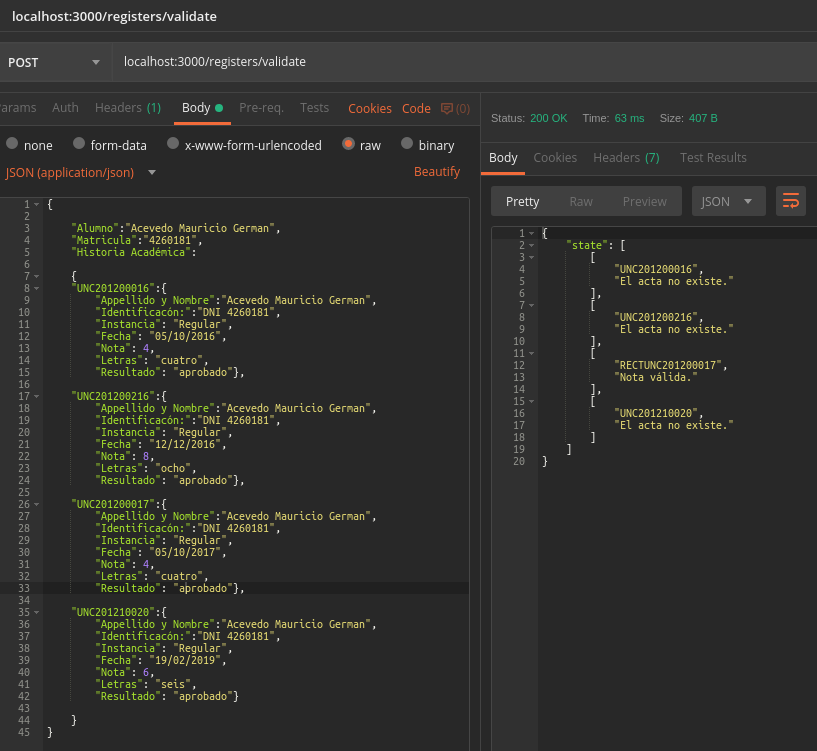
\includegraphics[width=0.9\linewidth]{Figures/Selection_226.png}}
    \caption{Validación de una historia académica involucrando un acta rectificativa.}
    \label{fig:history_with_revoked}
\end{figure}
\subsubsection{Desarrollo de la función \textit{query\_rectified}}
La función es implementada de la misma forma que \textit{query}, pero invoca al \textit{chaincode} \textit{queryAllRectified}, el cual tiene la particularidad de filtrar todas las actas con el prefijo ``RECT''. En la captura \ref{fig:all_rectified}, aparece solo un acta, porque en el momento de la prueba no se habían cargado y revocado más actas, sin embargo siempre figurará la cantidad correspondiente a las actas rectificadas.
\begin{figure}
    \center{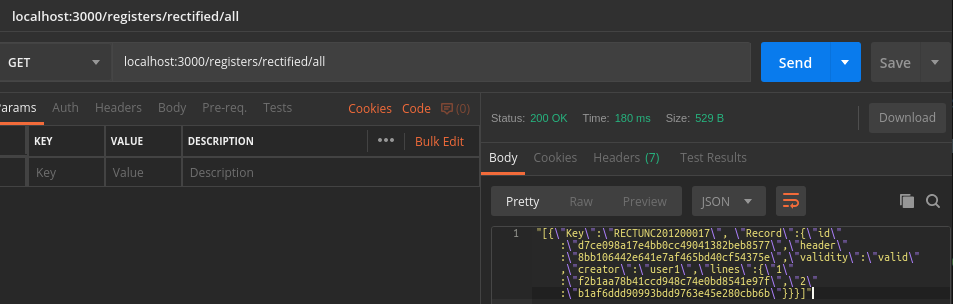
\includegraphics[width=0.9\linewidth]{Figures/Selection_227.png}}
    \caption{Consulta por todas las actas rectificativas.}
    \label{fig:all_rectified}
\end{figure}
\subsection{Implementación del Frontend con Angular e Ionic}
Luego de las instalaciones de Angular e Ionic descritas en la sección \ref{instalation_frontend} se procedió a eliminar el contenido por defecto que lleva la aplicación de prueba. Luego, se siguieron los siguientes pasos de desarrollo:
\begin{itemize}
    \item Con la ayuda del comando
    \begin{minted}{bash}
$ ionic generate page <pagename>
    \end{minted}
se generaron en total 6 páginas, una por cada caso de uso.
    \item El objetivo de la página principal, \textit{home}, es proveer una visión general de las funcionalidades de la implementación. Para eso se utilizó la estructura \textit{ion-grid}, donde cada cuadrícula presenta uno de los casos de uso descritos. Se agregaron imágenes descriptivas para facilitar la navegación por la página. En la figura \ref{fig:home_page}, se puede ver dicha implementación.
    \begin{figure}[H]
        \center{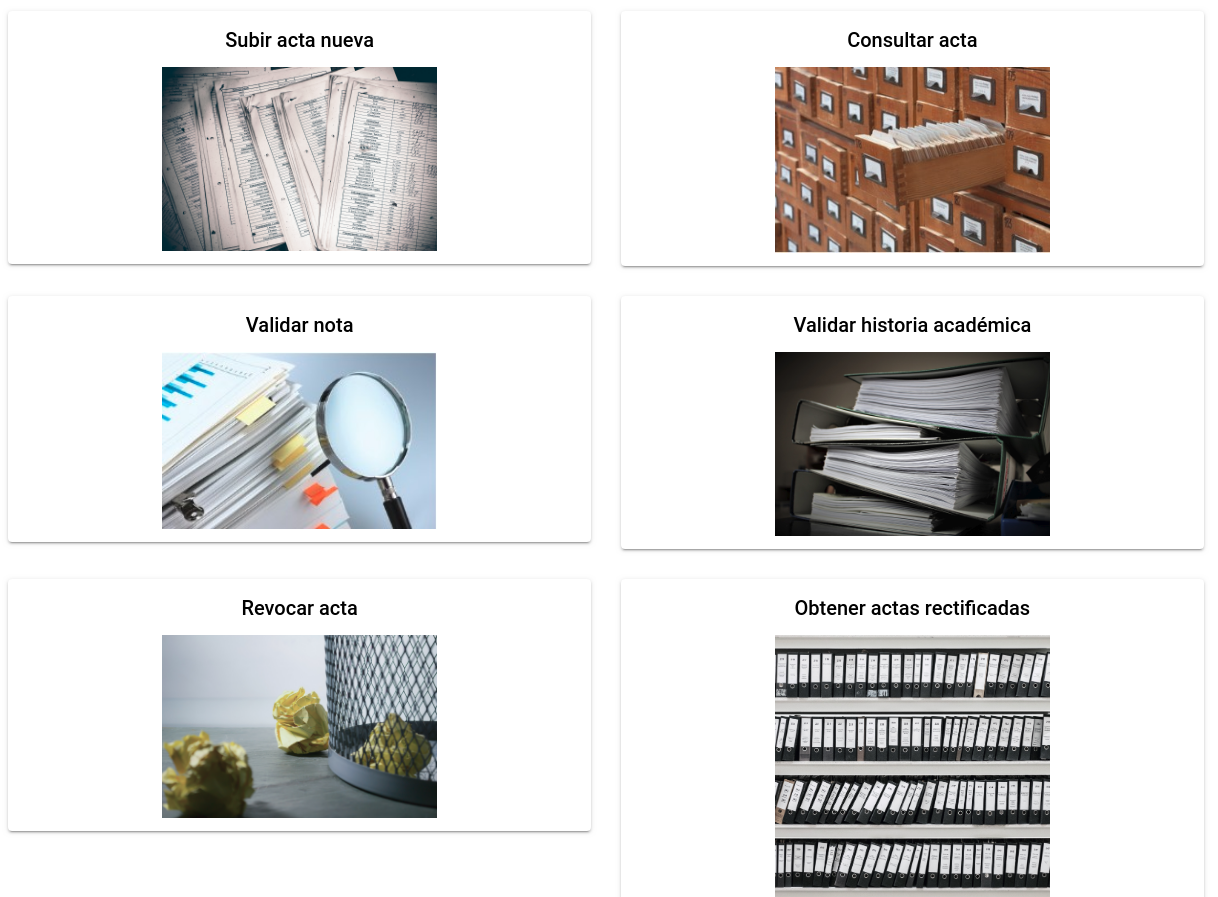
\includegraphics[width=0.7\linewidth]{Figures/Selection_228.png}}
        \caption{\textit{ion-grid} con los 6 casos de uso.}
        \label{fig:home_page}
    \end{figure}
    \item Al hacer clic en cada una de las cuadrículas, el usuario navega hacia la página correspondiente al caso de uso elegido. Ahí es presentado con un campo para una entrada de usuario, implementada mediante el componente \textit{ion-input}. Como en la mayoría de los casos la entrada del usuario tiene que tener formato JSON para ser enviada a la API, se verifica que los datos aportados realmente tengan dicho formato. En caso contrario, indica un error mediante el componente \textit{ion-toast} y la API no es invocada. Dicho caso se puede ver en la figura \ref{fig:json_toast}
    \begin{figure}[H]
        \center{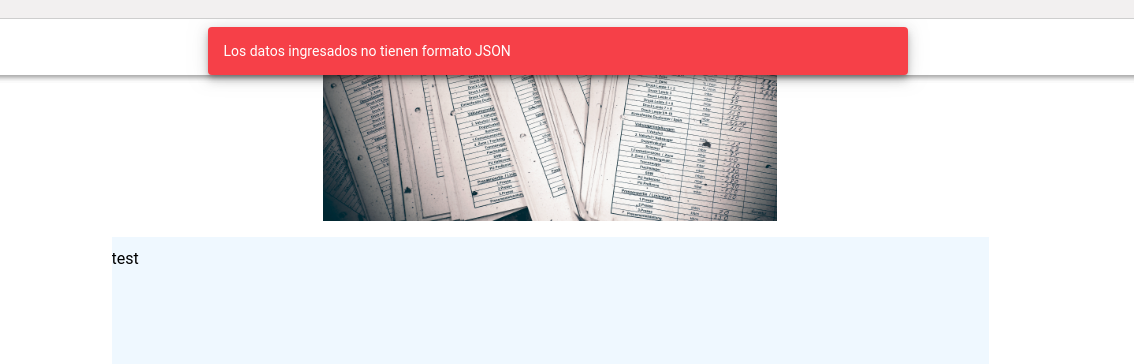
\includegraphics[width=0.8\linewidth]{Figures/Selection_229.png}}
        \caption{Un \textit{ion-toast} que indica que la entrada de usuario no se encuentra en formato JSON.}
        \label{fig:json_toast}
    \end{figure}
    \item Para notificar al usuario si los datos ingresados se escribieron exitosamente en el Blockchain, se empleó el componente \textit{ion-alert}. Dicho elemento abre una pequeña ventana que indica el éxito o fracaso de una operación y provee un mensaje de error si es necesario. En la figura \ref{fig:ion_alert} se muestran dos posibles alertas: en el primer caso, un acta se agregó exitosamente al Blockchain. Al querer subir la misma acta nuevamente, se produce el error visible a la derecha: si bien se pudo acceder al Blockchain, no fue posible escribir en él ya que el acta existía anteriormente.
    \begin{figure}[H]
        \center{
\includegraphics[width=0.8\linewidth]{Figures/Selection_232.png}}
        \caption{Alertas de notificación sobre el éxito o fracaso de una operación.}
        \label{fig:ion_alert}
    \end{figure}
    \item Para que los usuarios que desconocen el sistema puedan utilizar el mismo, se generó una página adicional de ayuda, que provee instrucciones y ejemplos.
    \item Por último, se agregó la funcionalidad de traducción de la página web con el módulo @ngx-translate/core. En la parte superior se encuentran la bandera española junto a la bandera estado-unidense. Seleccionar la bandera a elección modifica el idioma en el que aparece la página.
\end{itemize}

%\section{Implementación en un clúster Kubernetes}
%\subsection{Migración de Hyperledger Fabric}
%\subsection{Migración de la Aplicación}
%\subsection{Migración del Frontend}

 
% \chapter{Pruebas y Validación} % Main chapter title
\label{Chapter6}
\lhead{Capítulo 6. \emph{Pruebas y Validación}}
\setstretch{1.1} % Line spacing of 1.1
En el presente capítulo se describen los procedimientos de prueba para los requerimientos descritos en el cuadro \ref{table:req_user}. Cada uno de los cuadros visibles a continuación describe el objetivo de la prueba, el procedimiento, el resultado esperado y el estado final, que indican si la prueba se realizó de forma exitosa o no. Por último, en el capítulo se encuentra una matriz de trazabilidad que permite relacionar los requerimientos de usuario con los requerimientos funcionales y asociar cada uno con su caso de prueba correspondiente.
\section{Validación de los requerimientos de usuario}
\renewcommand{\tabularxcolumn}[1]{>{\arraybackslash}m{#1}}
% prueba req1
\begin{table}[H]
    \rowcolors{2}{gray!20}{white}
    \begin{tabularx}{\textwidth}{|m{3cm}|X|}
    \hline
    Id & TC-01\\
    \hline
    Título & Creación de un acta nueva en el Blockchain \\
    \hline
    Objetivo & Demostrar el funcionamiento correcto de la carga de actas al Blockchain.\\
    \hline
    Procedimiento & \begin{enumerate}
        \item El usuario debe dirigirse hacia la página y hacer clic en el cuadro con el título ``Subir acta nueva''.
        \item Luego debe ingresar el acta en el campo de texto previsto y hacer clic en el botón ``Subir acta''.
        \item Después de un tiempo de espera una alerta indicará si el acta pudo ser subida exitosamente o no.
    \end{enumerate}\\
    \hline
    Resultados esperados & Luego de un tiempo de espera, un cartel indicará el éxito de la operación. En el caso que el acta fue subida anteriormente y ya existe, indicará con un mensaje de error que el acta no pudo ser agregada.\\
    \hline
    Estado & Aprobado\\
    \hline
    \end{tabularx}
    \caption{Caso de prueba TC-01}
\end{table}
%prueba req 2
\begin{table}[H]
\rowcolors{2}{gray!20}{white}
\begin{tabularx}{\textwidth}{|m{3cm}|X|}
\hline
Id & TC-02\\
\hline
Título & Consulta de un acta en el Blockchain \\
\hline
Objetivo & Recuperar el acta del Blockchain con sus renglones en formato de \textit{hash}, tal como se subió.\\
\hline
Procedimiento & \begin{enumerate}
    \item El usuario debe dirigirse hacia la página y hacer clic en el cuadro con el título ``Consultar acta''.
    \item Luego debe ingresar el id del acta en el campo de texto previsto y hacer clic en el botón ``Obtener''.
\end{enumerate}\\
\hline
Resultados esperados & En el caso de que el acta exista, el contenido de la misma aparece debajo del botón, indicando los campos de la cabecera y los renglones. En el caso de no existir el acta, una alerta proporciona dicha información al usuario. Capturas de ambos casos se encuentran en las figuras \ref{fig:query_success} y \ref{fig:query_failure}.\\
\hline
Estado & Aprobado\\
\hline
\end{tabularx}
\caption{Caso de prueba TC-02}
\end{table}

\begin{figure}[H]
    \center{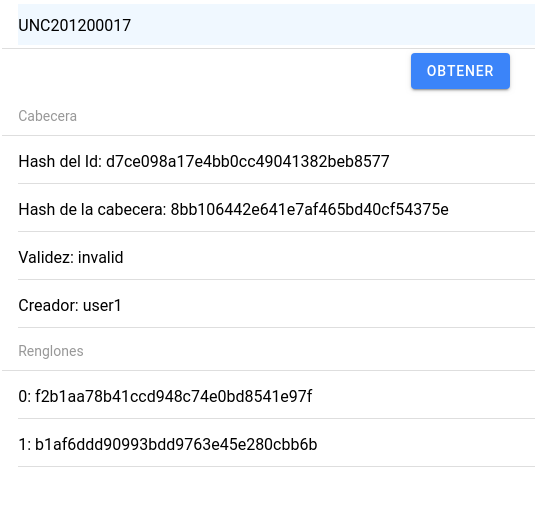
\includegraphics[width=0.8\linewidth]{Figures/Selection_234.png}}
    \caption{Alertas de notificación sobre el éxito o fracaso de una operación.}
    \label{fig:query_success}
\end{figure}

\begin{figure}[H]
    \center{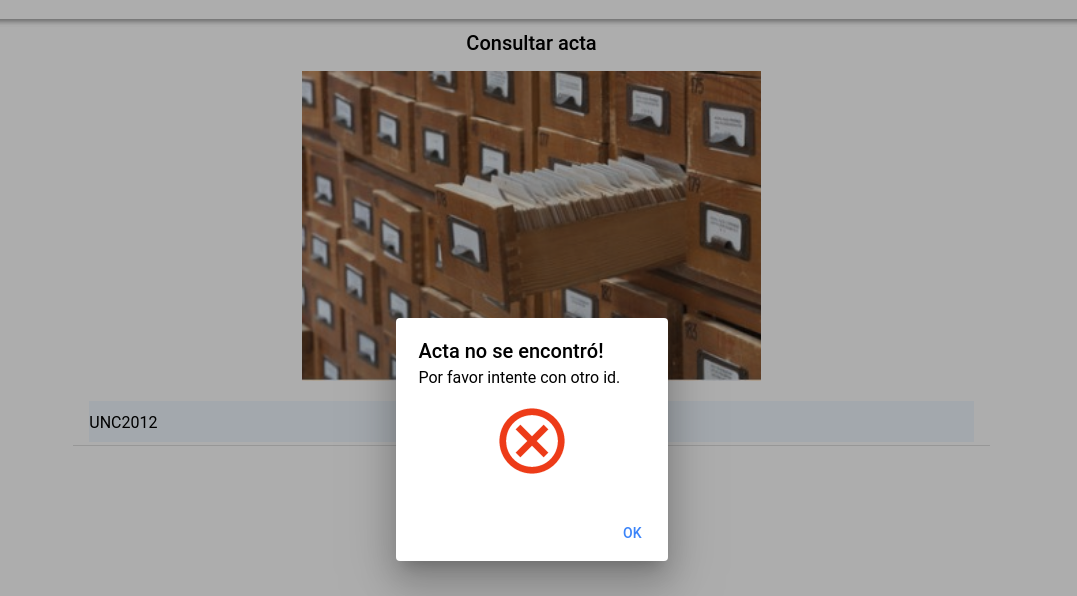
\includegraphics[width=0.8\linewidth]{Figures/Selection_233.png}}
    \caption{Alertas de notificación sobre el éxito o fracaso de una operación.}
    \label{fig:query_failure}
\end{figure}

%prueba req 3
\begin{table}[H]
\rowcolors{2}{gray!20}{white}
\begin{tabularx}{\textwidth}{|m{3cm}|X|}
\hline
Id & TC-03\\
\hline
Título & Validación de una nota con el Blockchain \\
\hline
Objetivo & Obtener información sobre la validez o invalidez de una nota.\\
\hline
Procedimiento & \begin{enumerate}
    \item El usuario debe dirigirse hacia la página y hacer clic en el cuadro con el título ``Validar nota''.
    \item Luego debe ingresar toda la información correspondiente en el campo de texto previsto y hacer clic en ``Validar''.
    \item Después de un tiempo de espera una alerta indicará si la nota es válida o no.
\end{enumerate}\\
\hline
Resultados esperados & Un cartel indica si la nota es válida, si no es válida o que el acta en el cual se tenía que encontrar la nota no existe.\\
\hline
Estado & Aprobado\\
\hline
\end{tabularx}
\caption{Caso de prueba TC-03}
\end{table}

%prubea requerimiento 4
\begin{table}[H]
\rowcolors{2}{gray!20}{white}
\begin{tabularx}{\textwidth}{|m{3cm}|X|}
\hline
Id & TC-04\\
\hline
Título & Validación de una historia académica \\
\hline
Objetivo & Obtener información sobre la validez o invalidez de una historia académica.\\
\hline
Procedimiento & \begin{enumerate}
    \item El usuario debe dirigirse hacia la página y hacer clic en el cuadro con el título ``Validar historia académica''.
    \item Luego debe ingresar toda la información correspondiente en el campo de texto previsto y hacer clic en ``Validar''.
    \item Después de un tiempo de espera, la página indicará si la historia académica es válida o no.
\end{enumerate}\\
\hline
Resultados Esperados & Como en el caso de la validación de una sola nota, un cartel indica la validez o invalidez de la historia académica. Por debajo del botón ``Validar'' aparece una lista con los ids de las actas que se consultó y el resultado por cada acta. En la figura \ref{fig:academic_history_fail} se puede ver un ejemplo donde no se logró validar una historia académica, junto con el detalle de los errores de las notas que no se lograron validar. \\
\hline
Estado & Aprobado\\
\hline
\end{tabularx}
\caption{Caso de prueba TC-04}
\end{table}

\begin{figure}[H]
    \center{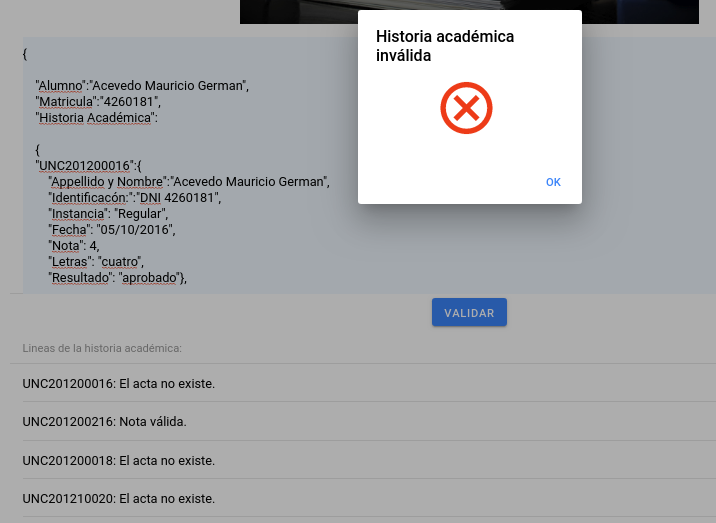
\includegraphics[width=0.8\linewidth]{Figures/Selection_235.png}}
    \caption{Caso de una historia académica inválida.}
    \label{fig:academic_history_fail}
\end{figure}

%prubea requerimiento 5
\begin{table}[H]
\rowcolors{2}{gray!20}{white}
\begin{tabularx}{\textwidth}{|m{3cm}|X|}
\hline
Id & TC-05\\
\hline
Título & Revocar un acta \\
\hline
Objetivo & Corroborar el funcionamiento correcto del sistema al revocar una acta.\\
\hline
Procedimiento & \begin{enumerate}
    \item El usuario debe dirigirse hacia la página y hacer clic en el cuadro con el título ``Revocar acta''.
    \item Luego debe ingresar toda la información correspondiente en el campo de texto previsto y hacer clic en el botón ``Revocar acta''.
    \item Después de un tiempo de espera, la página indicará si el acta pudo ser revocada o no.
\end{enumerate}\\
\hline
Resultados Esperados & En el caso de una revocación inválida, es decir, en el caso que el acta a revocar no existe o ya es inválida, el sistema devuelve un error. Si se puede revocar al acta, el sistema avisa después de un tiempo de espera que el acta pudo ser revocada correctamente.\\
\hline
Estado & Aprobado\\
\hline
\end{tabularx}
\caption{Caso de prueba TC-05}
\end{table}


%prueba req 6
\begin{table}[H]
\rowcolors{2}{gray!20}{white}
\begin{tabularx}{\textwidth}{|m{3cm}|X|}
\hline
Id & TC-06\\
\hline
Título & Consulta de las actas rectificadas\\
\hline
Objetivo & Recuperar información sobre todas las actas rectificadas existentes en el Blockchain.\\
\hline
Procedimiento & \begin{enumerate}
\item El usuario debe dirigirse hacia la página y hacer clic en el cuadro con el título ``Obtener actas rectificadas''.
\item En la página, debe hacer clic en el botón ``Obtener actas rectificadas''.
\end{enumerate}\\
\hline
Resultados esperados & En el caso de no existir ningún acta rectificada, la página muestra un texto indicando lo mismo. Si existen actas rectificadas, en una lista se detallan id, \textit{hash} del id, \textit{hash} de la cabecera, la validez del acta como el usuario que lo creó. \\
\hline
Estado & Aprobado\\
\hline
\end{tabularx}
\caption{Caso de prueba TC-06}
\end{table}

\lstset{
  frame=none
}
%prueba 7
\begin{table}[H]
    \rowcolors{2}{gray!20}{white}
    \begin{tabularx}{\textwidth}{|m{3cm}|X|}
    \hline
    Id & TC-07\\
    \hline
    Título & Presencia de Organizaciones y CA's\\
    \hline
    Objetivo & Verificar que existen los \textit{peers} y autoridades de certificación especificados en los requerimientos.\\
    \hline
    Procedimiento & \begin{enumerate}
    \item En la máquina de desarrollo local, ejecutar el comando 
    \begin{lstlisting}^^J
        $ docker ps^^J
    \end{lstlisting}
    \item En el cluster de Kubernetes, ejecutar el comando
    \begin{lstlisting}^^J
        $ kubectl get pods^^J
    \end{lstlisting}
    \end{enumerate}\\
    \hline
    Resultados esperados & Los contenedores o \textit{pods} que están presentes se pueden ver también en la figura \ref{fig:all_containers}: Se pueden encontrar \textit{peer0} como \textit{peer1} de cada organización y los tres contenedores que funcionan como una autoridad de certificación.\\
    \hline
    Estado & Aprobado\\
    \hline
    \end{tabularx}
    \caption{Caso de prueba TC-07}
    \end{table}

\begin{figure}[H]
    \center{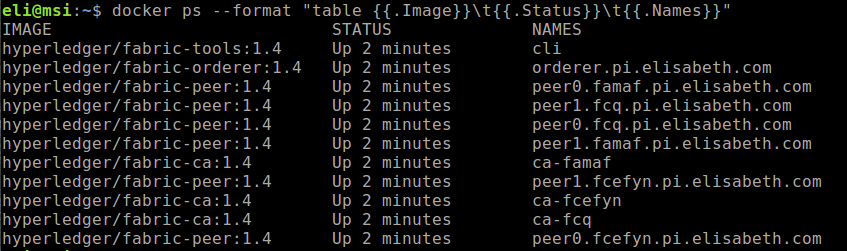
\includegraphics[width=1.0\linewidth]{Figures/Selection_237.png}}
    \caption{Los contenedores que deben estar presentes para cumplir con los requerimientos RF-BC-01 y RF-BC-03. }
    \label{fig:all_containers}
\end{figure}

%prueba 8
\begin{table}[H]
    \rowcolors{2}{gray!20}{white}
    \begin{tabularx}{\textwidth}{|m{3cm}|X|}
    \hline
    Id & TC-08\\
    \hline
    Título & Traducción de la página al inglés\\
    \hline
    Objetivo & Verificar que el \textit{frontend} está disponible en los idiomas inglés y español.\\
    \hline
    Procedimiento & \begin{enumerate}
    \item En la máquina de desarrollo local, ingresar la URL donde está funcionando la aplicación de Angular, en este caso, \textit{http://localhost:8100/home}.
    %\item Para el caso del despliege de Kubernetes, dirigirse hacía el dominio al cual está apuntando el ingrés del cluster.
    \item En la esquina superior derecha de la página, se encuentran una bandera española y una bandera estadounidense. El idioma por defecto es español: Para cambiar al inglés, es necesario hacer clic en la bandera estadounidense.
    \end{enumerate}\\
    \hline
    Resultados esperados & El idioma de toda la página cambia del español al inglés y vice versa al elegir la bandera correspondiente. En la figura \ref{fig:language_change} puede ver el cambio para el caso del título en la página principal.\\
    \hline
    Estado & Aprobado\\
    \hline
    \end{tabularx}
    \caption{Caso de prueba TC-08}
    \end{table}

    \begin{figure}[H]
        \center{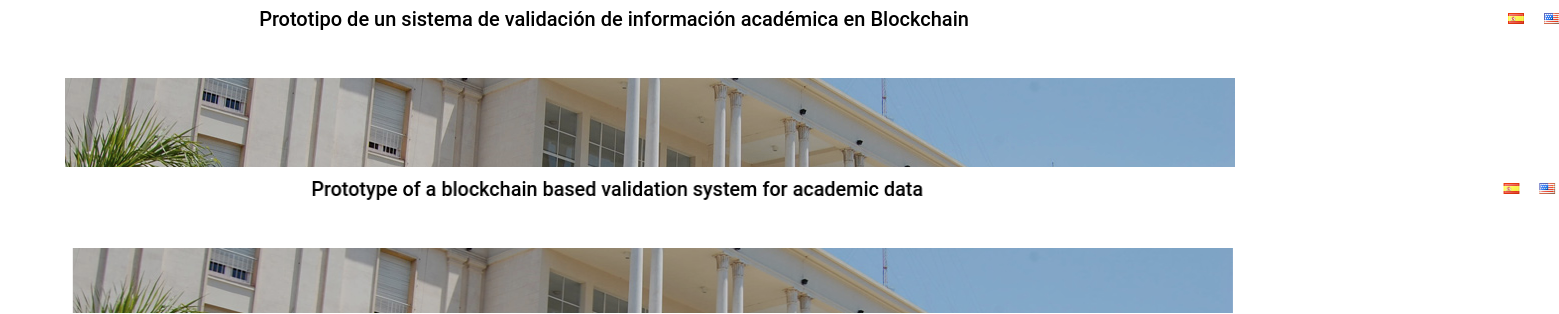
\includegraphics[width=1.0\linewidth]{Figures/Selection_238.png}}
        \caption{Prueba de cambio de idioma en la página principal.}
        \label{fig:language_change}
    \end{figure}

% prubea 9
\begin{table}[H]
    \rowcolors{2}{gray!20}{white}
    \begin{tabularx}{\textwidth}{|m{3cm}|X|}
    \hline
    Id & TC-09\\
    \hline
    Título & Prueba de la página de ayuda\\
    \hline
    Objetivo & Comprobar que un usuario sin conocimiento previo del uso de la página sea capaz de utilizarla.\\
    \hline
    Procedimiento & \begin{enumerate}
    \item Guiar al usuario a la página de ayuda y pedir que lea cuidadosamente las instrucciones.
    \item Pedir al usuario que agregue un acta nueva según las instrucciones y que luego valide una nota de dicha acta. 
    \end{enumerate}\\
    \hline
    Resultados Esperados & Suponiendo el correcto funcionamiento de frontend, API y Blockchain, el usuario no debe tener ningún inconveniente en realizar lo pedido. Para el caso de personas que no tienen ningún conocimiento previo de programación, se anticipan confusiones con la redacción del acta en formato JSON.\\
    \hline
    Estado & Aprobado\\
    \hline
    \end{tabularx}
    \caption{Caso de prueba TC-09}
    \end{table}
\section{Matriz de trazabilidad}
En la matriz visible a continuación se relacionan todos los requerimientos planteados con los casos de test descritos en la sección anterior, con la finalidad de obtener una visión general que todos los requerimientos fueron testeados exitosamente. Los requerimientos no funcionales RNF-01 (El sistema debe contar con pruebas y tests integrales de los seis requerimientos de usuario.) y RNF-02 (El código del \textit{chaincode} debe estar escrito en Golang, la API debe desarrollarse en Node.js y para la interfaz gráfica se debe usar Typescript.) no figuran en la tabla, ya que establecen metodologías y herramientas de trabajo.

\newcommand*\rot{\rotatebox{90}}
\newcommand*\OK{\ding{51}}


\begin{table}[h]
    \begin{adjustwidth}{-1.5cm}{}
    \begin{tabular}{c|cccccc|cccccc|ccccc|cc|}
        &
        \rot{RF-BC-01 } &
        \rot{RF-BC-02 } &
        \rot{RF-BC-03 } &
        \rot{RF-BC-04 } &
        \rot{RF-BC-05 } &
        \rot{RF-BC-06 } &
        \rot{RF-API-01 } &
        \rot{RF-API-02 } &
        \rot{RF-API-03 } &
        \rot{RF-API-04 } &
        \rot{RF-API-05 } &
        \rot{RF-API-06 } &
        \rot{RF-GUI-01 } &
        \rot{RF-GUI-02 } &
        \rot{RF-GUI-03 } &
        \rot{RF-GUI-04 } &
        \rot{RF-GUI-05 } &
        \rot{RNF-03 } &
        \rot{RNF-04 } \\
    \hline
    TC-01 & & \cellcolor{YellowGreen!55}\OK & & \cellcolor{YellowGreen!55}\OK & \cellcolor{YellowGreen!55} \OK &
    \cellcolor{YellowGreen!55} \OK & \cellcolor{YellowGreen!55} \OK & & & & & \cellcolor{YellowGreen!55} \OK & \cellcolor{YellowGreen!55} \OK &\cellcolor{YellowGreen!55} \OK & & \cellcolor{YellowGreen!55} \OK & \cellcolor{YellowGreen!55} \OK & \cellcolor{YellowGreen!55} \OK & \\
    \hline
    TC-02 & & & & \cellcolor{YellowGreen!55}\OK & & \cellcolor{YellowGreen!55} \OK &
    & \cellcolor{YellowGreen!55} \OK & & & & \cellcolor{YellowGreen!55} \OK & \cellcolor{YellowGreen!55} \OK & \cellcolor{YellowGreen!55} \OK &  & \cellcolor{YellowGreen!55} \OK & \cellcolor{YellowGreen!55} \OK & \cellcolor{YellowGreen!55} \OK & \\
    \hline
    TC-03 & & & & \cellcolor{YellowGreen!55}\OK & & \cellcolor{YellowGreen!55} \OK &
     & & \cellcolor{YellowGreen!55} \OK & & & \cellcolor{YellowGreen!55} \OK & \cellcolor{YellowGreen!55} \OK & \cellcolor{YellowGreen!55} \OK & & \cellcolor{YellowGreen!55} \OK & \cellcolor{YellowGreen!55} \OK & \cellcolor{YellowGreen!55} \OK & \\
    \hline
    TC-04 & & & & \cellcolor{YellowGreen!55}\OK & & \cellcolor{YellowGreen!55} \OK &
    & & & \cellcolor{YellowGreen!55} \OK & & \cellcolor{YellowGreen!55} \OK & \cellcolor{YellowGreen!55} \OK & \cellcolor{YellowGreen!55} \OK & & \cellcolor{YellowGreen!55} \OK & \cellcolor{YellowGreen!55} \OK & \cellcolor{YellowGreen!55} \OK & \\
    \hline
    TC-05 & & \cellcolor{YellowGreen!55}\OK & & \cellcolor{YellowGreen!55}\OK & \cellcolor{YellowGreen!55} \OK &
    \cellcolor{YellowGreen!55} \OK &
    & & & & \cellcolor{YellowGreen!55} \OK & \cellcolor{YellowGreen!55} \OK & \cellcolor{YellowGreen!55} \OK & \cellcolor{YellowGreen!55} \OK &  & \cellcolor{YellowGreen!55} \OK & \cellcolor{YellowGreen!55} \OK & \cellcolor{YellowGreen!55} \OK & \\
    \hline
    TC-06 & & & & \cellcolor{YellowGreen!55}\OK & & \cellcolor{YellowGreen!55} \OK &
    & \cellcolor{YellowGreen!55} \OK & & & & \cellcolor{YellowGreen!55} \OK & \cellcolor{YellowGreen!55} \OK & \cellcolor{YellowGreen!55} \OK &  & \cellcolor{YellowGreen!55} \OK & \cellcolor{YellowGreen!55} \OK & \cellcolor{YellowGreen!55} \OK & \\
    \hline
    TC-07 & \cellcolor{YellowGreen!55} \OK & & \cellcolor{YellowGreen!55} \OK & & & &
     & & & & & &
     & & & &
     & & \\
    \hline
    TC-08 & & & & & & &
     & & & & & &
     & & \cellcolor{YellowGreen!55} \OK & &
     & & \\
    \hline
    TC-09 & & & & & & &
     & & & & & &
     & & & &
     & & \cellcolor{YellowGreen!55} \OK \\
    \hline
    \end{tabular}
\end{adjustwidth}
\caption{Matriz de trazabilidad}
\end{table}
% %\chapter{Análisis de Costos} % Main chapter title
\label{Chapter7}
\lhead{Capítulo 7. \emph{Análisis de Costos}}
\setstretch{1.1} % Line spacing of 1.1
pequeña introducción

1. costo de un despliegue en hardware
2. costo de un despliegue en la solución de blockchain de AWS
3. costo de despliegue en la solución de K8 de AWS
lo mismo para IBM?
 
% \chapter{Conclusión} % Main chapter title
\label{Chapter7}
\lhead{Capítulo 7. \emph{Conclusión}}
\setstretch{1.1} % Line spacing of 1.1

En el presente proyecto, se realizó un estudio profundo de la tecnología Blockchain, sus características más importantes como también sus aplicaciones y casos de uso. Se comparó una multitud de plataformas Blockchain diferentes. Luego, se eligió una plataforma de las analizadas para probar su funcionamiento en un caso práctico que no involucrara la necesidad de una criptomoneda. Se investigó la utilidad de un sistema de validación de actas académicas y se llegó a la conclusión que un sistema con arquitectura Blockchain puede superar en utilidad a un sistema de base de datos tradicional.

Después de la etapa de investigación se procedió a desarrollar un prototipo con el fin de evaluar la implementabilidad y utilidad de la propuesta. Para eso, el proyecto se dividió en tres partes: 

\begin{enumerate}
    \item La primera parte consiste en la configuración de la red Blockchain con el framework elegido. Se configuraron 3 organizaciones diferentes con 2 nodos cada una, que comparten el mismo canal y usan el mecanismo de aprobación de transacciones \textit{solo}. Ambos nodos por cada organización funcionan como nodos de aprobación de transacciones y un nodo por cada organización se configuró adicionalmente como \textit{anchor node} para posibilitar el descubrimiento de nodos de otras organizaciones. El desarrollo del \textit{chaincode} permite agregar y modificar información al Blockchain, una vez que toda la red fue iniciada.
    \item La segunda parte consiste en la programación de la API con la ayuda del SDK previsto por Hyperledger Fabric. Se implementaron los diferentes \textit{endpoints} que invocan al \textit{chaincode} correspondiente, el cual consulta por información existente o agrega información nueva. Se implementaron las siguientes funcionalidades:
    \begin{enumerate}
        \item Subir un acta nueva.
        \item Consultar por un acta subida.
        \item Validar una nota.
        \item Validar una historia académica.
        \item Rectificar un acta.
        \item Consultar por todas las actas rectificadas.
    \end{enumerate}
    \item En la última parte, se desarrolló una aplicación web para que el usuario pueda interactuar con el sistema a través de una interfaz gráfica. Con Angular, se crearon diferentes páginas que interactúan con la API y dan una retroalimentación visual al usuario para indicar si su operación fue exitosa o fracasó.
\end{enumerate}

\section{Problemas y Limitaciones}
A continuación, se elaboran algunos problemas y limitaciones que se presentaron durante el desarrollo del proyecto.

\begin{itemize}
    \item 
    En el momento de la investigación, resultó difícil encontrar bibliografía. Dado que la primera implementación de una arquitectura Blockchain data en el 2009, es un tema reciente, y no existen libros que discuten el tema con la profundidad requerida. Por otro lado, especialmente gracias a las criptomonedas, es un tema polémico que atrae mucha atención, y se encuentran muchas fuentes con información erronea. Por esa razón, se aplicaron criterios rigurosos para su elección: la mayoría de la información fue extraida de papers científicos, blogs de fundadores de implementaciones Blockchain y de la documentación de dichas implementaciones.
    \item Una vez elegido el \textit{framework} Hyperledger Fabric para la implementación del trabajo, se presentarion una multitud de problemas y dudas que solo se lograron resolver en parte: Si bien se encontraron preguntas relacionadas en foros como Stackoverflow, para muchas existen pocas respuestas o ninguna. Para esos casos, fue necesario asumir o experimentar con ejemplos hasta llegar a una conclusión satisfactoria.
    \item Todos los proyectos de Hyperledger son gestionados por la Linux Foundation y son proyectos de código libre, donde se modifican y agregan funcionalidades constantemente. \textit{Bugs} en versiones que se usaron en este proyecto se resolvieron al migrar a versiones posteriores, las cuales, sin embargo, introducían funcionalidades desconocidas que todavía no contaban con la documentación necesaria y a veces introducían otros problemas o incompatibilidades imprevistas.  
\end{itemize}

\section{Trabajos futuros}
A continuación, figuran algunas mejoras y extensiones al presente proyecto, que no se implementaron por limitaciones de tiempo o porque su desarrollo se desviaba del objetivo inicial del proyecto integrador.

Mejoras propuestas en la parte de interfaz gráfica y API:
\begin{itemize}
    \item Agregar autenticación de usuarios a la aplicación web, para que solamente personal autorizado pueda agregar y revocar actas.
    \item Junto con la autenticación, implementar una limitación para que un acta solamente puede ser rectificado por el mismo usuario que lo creó originalmente.
    \item Implementar que cada acta del sistema sea firmada digitalmente por su creador.
    \item Desarrollar una planilla en la interfaz gráfica que permita ingresar los datos requeridos a través de un formulario en vez de usar el formato JSON. Para un usuario poco experimentado con la computación, respetar el formato JSON puede resultar engorroso.
    \item Para una adopción más fácil de la tecnología y mitigar el riesgo de un usuario vacilante, también es posible automatizar la obtención de los datos del alumno, de tal manera que la aplicación utilice una API del sistema Guaraní para obtener la información en texto plano, en vez de requerir su ingreso manual en formato JSON. Sin embargo, es primordial tener en cuenta que el alumno antes debe autorizar dicho acceso, ya que su información no debe ser difundida sin su consentimiento.
\end{itemize}

Mejoras propuestas en la parte de la red Blockchain:
\begin{itemize}
    \item Desplegar la red con más que un nodo de aprobación de transacciones para lograr redundancia usando Raft o Kafka.
    \item Desplegar una mayor cantidad de nodos por organización: Para ambientes de producción, Hyperledger Fabric recomienda un mínimo de tres nodos por organización, de los cuales dos deben estar configurados como \textit{anchor peers}.
    \item Generar las identidades digitales a través de las CA en vez de utilizar la herramienta cryptogen, ya que ésta predefine la topología de la red y una modificación posterior resulta complicada.
    \item Realizar un análisis de costos de un despliegue en producción.
\end{itemize}


\section{Aporte personal}
El conocimiento adquirido a lo largo de la carrera, especialmente en las materias de los últimos años como Bases de Datos, Redes de Computdoras y Sistemas Operativos, formó una base de conocimiento imprescindible para el desarrollo del proyecto. Si bien los paradigmas en cuestión recién cumplen 10 años, los problemas que se plantearon pudieron ser abarcados gracias a la preparación recibida en la facultad junto con paciencia, perseverancia y curiosidad. 


%----------------------------------------------------------------------------------------
%	THESIS CONTENT - APPENDICES
%----------------------------------------------------------------------------------------

\addtocontents{toc}{\vspace{2em}} % Add a gap in the Contents, for aesthetics

\appendix % Cue to tell LaTeX that the following 'chapters' are Appendices

% Include the appendices of the thesis as separate files from the Appendices folder
% Uncomment the lines as you write the Appendices

%\input{Appendices/AppendixA}

\addtocontents{toc}{\vspace{2em}} % Add a gap in the Contents, for aesthetics

\backmatter

%% Chapter Template
\bibliographystyle{unsrtnat} % Use the "unsrtnat" BibTeX style for formatting the Bibliography

\chapter{Bibliografía} % Main chapter title

%\label{Bibliografia} % Change X to a consecutive number; for referencing this chapter elsewhere, use \ref{ChapterX}
%\section{Bibliografía}

\lhead{\emph{Bibliografía}} % Change X to a consecutive number; this is for the header on each page - perhaps a shortened title

\begin{itemize}
\item A Software Testing Primer: An Introduction to Software Testing.Jenkins, Nick.Año 2008.
\item Applying Agile Methods to Embedded Systems Development,Doug Dahlby,PhD,Applying Agile Methods to Embedded Systems Development,Año 2004.\\
	\href{url}{http://embuild.org/dahlby/agileEm/agileEm.pdf} \\
	Última fecha de consulta: 07/03/2016.
\item Andrés Djordjalian,Desarrollo Ágil y Modelado,Año 2010.\\
	\href{url}{http://www.indicart.com.ar/~sase/Desarrollo\%20Agil\%20y\%20Modelado.pdf}\\
	Última fecha de consulta: 	 07/03/2016.
\item IEEE Recommended Practice for Software Requirements Specifications,IEEE Computer Society,Año 1998.\\
	\href{url}{http://www.cse.msu.edu/~cse870/IEEEXplore-SRS-template.pdf}\\
	Última fecha de consulta: 	 07/03/2016.
\item Software Engineering for Students, 4ta edición,Douglas Bell,Addison-Wesley,ISBN:978-0-32126-127-4,Año 2005.
\item Agile Web Development with Rails,4ta edición,Sam Ruby,Dave Thomas,David Heinemeier Hansson,The Pragmatic Programmers LLC,2010.
\item Head First Rails,David Griffiths,O'reilly,ISBN:978-0-596-51577-5,Año 2009.
\item Sockets programming in Ruby,M. Tim Jones,Año 2005.\\
	\href{url}{https://www6.software.ibm.com/developerworks/education/l-rubysocks/l-rubysocks-a4.pdf}\\
	Última fecha de consulta: 	 07/03/2016.
\item Head First Ajax,Rebecca M. Riordan,O'reilly,ISBN:978-0-596-51578-2,Año 2008.
\item Head First Android Development,Jonathan Simon,O'reilly,ISBN:978-1-4493-9330-4,Año 2012.
\item Vanguard Security Corporation,Home Alarm System Design,Honeywell Security Products Dealer.
	\href{url}{http://www.diyalarms.net/system\_design.html}\\
	Última fecha de consulta: 	08/03/2016
\item Peter M. Rogers,Wireless Home Security 101 – How to Design Your Alarm System,HOME SECURITY BLOG,Frontpoint.\\
	\href{url}{http://blog.frontpointsecurity.com/wireless-home-security-101-how-to-design-your-alarm-system/}\\
	Última fecha de consulta: 	08/03/2016
\item Peter M. Rogers,Home Security 101: Wireless Home Alarm System Design Explained,HOME SECURITY BLOG,Frontpoint.\\
	 \href{url}{http://blog.frontpointsecurity.com/home-security-101-wireless-home-alarm-system-design-explained/}\\
	Última fecha de consulta: 	 08/03/2016
\item Stephen Cleary,TCP/IP Protocol Design: Message Framing,Code Projects.\\
	 \href{url}{http://www.codeproject.com/Articles/37496/TCP-IP-Protocol-Design-Message-Framing}\\
	Última fecha de consulta: 	 08/03/2016
\item Embedded Access Inc,Essentials of MQX RTOS Application Development.\\
	 \href{url}{http://www.nxp.com/support/online-academy/essentials-of-mqx-rtos-application-development:WBT\_MQX\_RTOS\_COURSE}\\
	Última fecha de consulta: 	 08/03/2016
\item Victor Costan,BSD Sockets in Ruby,Victor Costan\\	
	\href{url}{http://blog.costan.us/2007/09/bsd-sockets-in-ruby\_26.html}\\
	Última fecha de consulta: 	08/03/2016
\item Tutorialspoint,Ruby Socket Programming,Tutorialspoint.\\
	 \href{url}{http://www.tutorialspoint.com/ruby/ruby\_socket\_programming.htm}\\
	Última fecha de consulta: 	 08/03/2016
\item Ajain,Rich ,Ruby Socket: An Introduction to Ruby Sockets and Socket Programming.\\
	 \href{url}{https://blog.udemy.com/ruby-socket/}\\
	Última fecha de consulta: 	 08/03/2016
\item jwei,Incorporating Socket Programming into your Applications,Think Android.\\
	 \href{url}{https://thinkandroid.wordpress.com/}\\
	Última fecha de consulta: 	 08/03/2016
\item Maravitsas,Nikos,Android Socket Example,Java Code Geeks.\\
 \href{url}{https://examples.javacodegeeks.com/android/core/socket-core/android-socket-example/}\\
	Última fecha de consulta:  	08/03/2016
\item Suciu,Laura,Android TCP Connection Tutorial,My Android Solutions.\\
	 \href{url}{http://www.myandroidsolutions.com/2012/07/20/android-tcp-connection-tutorial/}\\
	Última fecha de consulta: 	08/03/2016
\item Tutoriales Android,Diploma de Especialización en desarrollo de aplicacione para Android.\\
	 \href{url}{http://www.androidcurso.com/index.php/tutoriales-android-fundamentos}\\
	Última fecha de consulta: 	 08/03/2016
\item Cipolat,Sebastian,Sockets en Android,Androideity.\\
	 \href{url}{http://androideity.com/2012/08/05/sockets-en-android/}\\
	Última fecha de consulta: 	 08/03/2016
\item Moisset,Diego,Android Ya(con Android Studio).\\
	 \href{url}{http://www.javaya.com.ar/androidya/androidstudioya/}\\
	Última fecha de consulta: 	 08/03/2016
\item Salvador Gómez, Oliver,SGOLIVER.NET,Curso Programación Android.\\
	 \href{url}{http://www.sgoliver.net/blog/curso-de-programacion-android/indice-de-contenidos/}\\
	Última fecha de consulta: 	 08/03/2016
\item Chui,Socket,Diang entre C y java,Ejemplos java y C/linux.\\
	 \href{url}{http://www.chuidiang.com/java/sockets/cpp\_java/cpp\_java.php}\\
	Última fecha de consulta: 	 08/03/2016
\item Launch School,Integrating Rails and Bootstrap.\\
	 \href{url}{https://launchschool.com/blog/integrating-rails-and-bootstrap-part-2/}\\
	Última fecha de consulta: 	 08/03/2016
\item Working with JavaScript in Rails, Rails Guides.\\
	 \href{url}{http://guides.rubyonrails.org/working\_with\_javascript\_in\_rails.html}\\
	Última fecha de consulta: 	 08/03/2016
\item Launch School,The Detailed Guide on How Ajax Works With Ruby on Rails.\\
	 \href{url}{https://launchschool.com/blog/the-detailed-guide-on-how-ajax-works-with-ruby-on-rails}\\
	Última fecha de consulta: 	 08/03/2016
\item Ruby on Rails - AJAX,Tutorialspoint.\\
	 \href{url}{http://www.tutorialspoint.com/ruby-on-rails/rails-and-ajax.htm}\\
	Última fecha de consulta: 	 08/03/2016
\item Hicham,AJAX Bootstrap Modals in Rails 4.\\
	 \href{url}{http://www.benkirane.ch/ajax-bootstrap-modals-rails/}\\
	Última fecha de consulta: 	 08/03/2016
\item ZetCode,Doing SQL queries with Ruby in SQLite.\\
	 \href{url}{http://zetcode.com/db/sqliteruby/queries/}\\
	 	Última fecha de consulta: 08/03/2016
\item Socket.\ \href{url}{http://ruby-doc.org/stdlib-2.0.0/libdoc/socket/rdoc/Socket.html}\\
	Última fecha de consulta: 	08/03/2016
\item CuriousInventor,designing PCBs in Kicad and PcbNew: Drawing Traces.\\
	 \href{url}{http://store.curiousinventor.com/guides/kicad/pcb\_layout/Draw\_traces}\\
	Última fecha de consulta: 	 08/03/2016
\item Module: Mail.\\	
	\href{url}{http://www.rubydoc.info/github/mikel/mail/Mail}\\
	Última fecha de consulta: 	08/03/2016
\end{itemize}

 
\lhead{\emph{Bibliografía}} % Change X to a consecutive number; this is for the header on each page - perhaps a shortened title

\bibliographystyle{IEEEtran}
\bibliography{Bibliography}
\end{document}\grid
